% !TEX TS–program = pdflatexmk    % for making citations with biber
% For copyright and license information, see uiucthesis2021.dtx and derivatives.
\documentclass[11pt]{./uiuc_thesis_template/uiucthesis2021} % Set global font here!
\usepackage[utf8]{inputenc}
\usepackage[english]{babel}
\usepackage{csquotes}
\usepackage{microtype}
\usepackage{amsmath,amsthm,amssymb}
\usepackage[bookmarksdepth=3,linktoc=all,colorlinks=true,urlcolor=blue,linkcolor=blue,citecolor=blue]{hyperref}
\usepackage[capitalize]{cleveref}
\usepackage[backend=biber, style=authoryear, citestyle=authoryear]{biblatex}

% User added packages
\usepackage{mathptmx}
\usepackage{color,soul}
\usepackage{upgreek}
\usepackage{graphicx}
\usepackage{caption}
\usepackage{siunitx}
\usepackage{booktabs}
%\usepackage{natbib}
\graphicspath{ {./figures/} }
%\usepackage[utf8]{inputenc}



%\usepackage{sectsty}
%\chapternumberfont{\Large} 
%\chaptertitlefont{\huge}

\usepackage{titlesec}
\titleformat{\chapter}[display]
{\normalfont\huge\bfseries}{\chaptertitlename\ \thechapter}{20pt}{\huge\onehalfspacing}
% this alters "before" spacing (the second length argument) to 0
\titlespacing*{\chapter}{0pt}{0pt}{40pt}

% \usepackage{ruledchapters}  % example of compliant heading format, uncomment to use

%\usepackage{lipsum}  % just for placeholder code

% uncomment the below to show a grid on all pages
% \usepackage[grid, gridunit=in, gridcolor=blue!40, subgridcolor=blue!20]{eso-pic}

\addbibresource{all-references.bib}

\newcounter{counterforappendices}

\begin{document}

\doublespacing

% ------------------------------------ TITLE PAGE --------------------------------------
\title{Idealized particle-resolved large-eddy simulations \\
to evaluate the impact of emissions spatial heterogeneity\\
on CCN activity}
\author{Samuel Frederick}
\department{Climate, Meteorology, and Atmospheric Sciences}
%\concentration{Coffee Studies}
\msthesis % options are \phdthesis or \msthesis
\degreeyear{2024}
\committee{
    Professor Nicole Riemer\\				% NOTE: use title of Dr. or professor?
    Professor Matthew West\\
    Professor Larry Di Girolamo}
\maketitle

\frontmatter

\begin{abstract}

% NOTE: abstract taken from CliMAS seminar... need to update!
Aerosol-cloud interactions remain a large source of uncertainty in climate models due to complex, nonlinear processes that alter aerosol properties and the inability to represent the full compositional complexity of aerosol populations within large-scale modeling frameworks. The spatial resolution of these models (typically 10-100 km) is often coarser than the spatially varying emissions in the modeled geographic region. This results in diffuse, uniform emission of primary aerosol and gas-phase species instead of spatially heterogeneous concentrations. Aerosol processes such as gas-particle partitioning and coagulation are concentration-dependent, and thus the representation of spatially heterogeneous emissions impacts aerosol aging and properties. This includes climate-relevant quantities like particle hygroscopicity and cloud condensation nuclei (CCN) activity. 

This thesis investigates the impact of emissions spatial heterogeneity on CCN activity by using the particle-resolved model PartMC coupled to the Weather Research and Forecasting model configured for large-eddy simulations (LES). The resulting modeling framework resolves turbulence-chemistry interactions and aerosol aging on a per-particle scale. The sensitivity of CCN activity to emissions spatial heterogeneity is evaluated for primary aerosol and gas-phase emissions typical of urban regions. The pattern of emissions is varied to investigate a range of spatially heterogeneity scenarios. For each scenario, CCN activity is compared against a uniform emissions base case to determine the impact of spatially heterogeneous emissions. 

\hl{TODO: update!} We find that CCN concentrations decrease by as much as 10\% with increasing emissions spatial heterogeneity, especially for low supersaturations (S=0.1, 0.3\%). This work is a first of a kind application of high resolution, particle-resolved LES for quantifying structural uncertainty of CCN activity due to the representation of emissions spatial heterogeneity.

\end{abstract} 

%\begin{dedication}
%To Father and Mother.
%\end{dedication}

\begin{acknowledgments}

\end{acknowledgments}

{
    \hypersetup{linkcolor=black}  % disable link coloring locally
    \setcounter{tocdepth}{2} % Does it matter if I go with 2 (includes subsections) or 1 (just chapters and sections)?
    \tableofcontents
    % the Graduate College doesn't recommend including lot or lof
     \listoftables
     \listoffigures
}

%\chapter{List of Abbreviations}

%\begin{abbrevlist}
%\item[BC] Black carbon
%\item[OC] Organic carbon
%\item[VOC] Volatile organic compound
%\end{abbrevlist}

%\chapter{List of Symbols}

%\begin{symbollist}[0.7in]
%\item[$\tau$] Time taken to drink one cup of coffee.
%\item[$\mu$g] Micrograms (of caffeine, generally).
%\end{symbollist}



\mainmatter

% !TEX root = ./main.tex
\chapter{Introduction}

This chapter discusses key background motivating this thesis, including fundamental properties of aerosols, their feedbacks on the climate, and the role of emissions spatial heterogeneity in altering the aerosol state. A description of the coupling between emissions spatial heterogeneity and aerosol processes is provided, and a brief review of current efforts to quantify and parameterize the sub-grid scale variability of aerosols is presented. Subsequently, the representation of aerosols in modeling frameworks is discussed and the current state of high-resolution coupled aerosol-transport models capable of resolving emissions spatial heterogeneity is reviewed. Finally, existing gaps in the literature are outlined and objectives are presented to answer primary avenues of inquiry in this thesis. 

\section{The complexity of atmospheric aerosols}\label{aerosol_properties}

An aerosol is a collection of particles composed of one or more chemical species that are suspended in a fluid or gas. In the atmosphere, aerosol particles vary considerably in terms of their physical properties such as size, composition, and origin. Additionally, the chemical, thermodynamic, and radiative properties of aerosol particles can alter the state of the aerosol and the surrounding environment through numerous feedback mechanisms. In turn, aerosol particles exhibit a complex, non-linear coupling with the environment that spans broad spatial and temporal scales.

\subsection{Particle size}

\begin{figure}[!t]
	\centering
	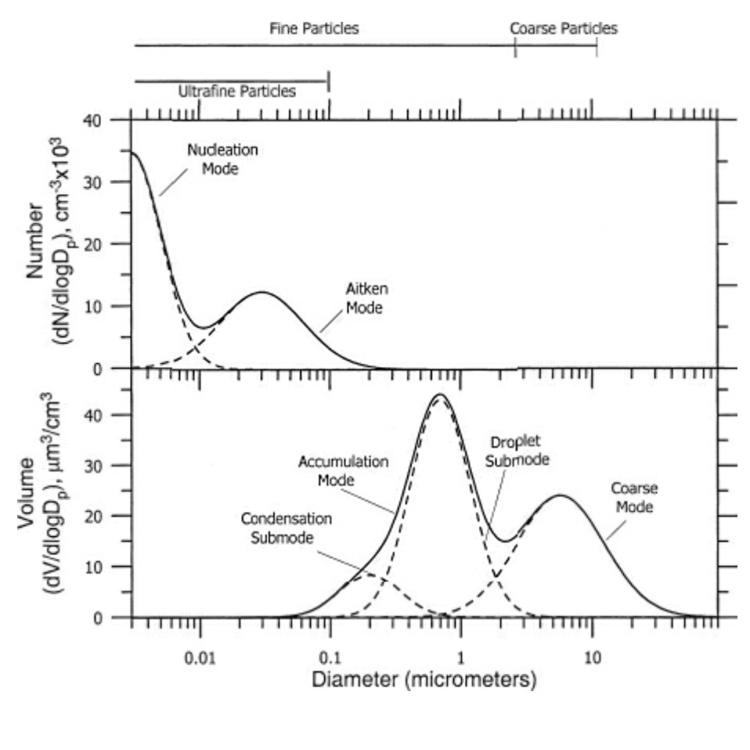
\includegraphics[width=.75\textwidth]{chapter1/SP_Figure_8-11.pdf}
	\caption{Common aerosol number and volume distributions organized by mode. Taken from \textcite{seinfeld_atmospheric_1998} with permission.}
	\label{fig:size_dists}
\end{figure} 

Aerosol particles are typically measured by their diameter where spherical morphology is assumed. The smallest particles have diameters on the order of 1~nm and are produced via the nucleation of low-volatility vapors. On the opposite extreme of particle sizes, the largest particle diameters can exceed 100~$\upmu$m. In total, aerosols span approximately five orders of magnitude \parencite{seinfeld_atmospheric_1998}. To capture the broad scale of particle diameters that may be present in a population of aerosol particles, aerosol size distributions often represent the number concentration of particles as a function of the logarithm of particle diameter. The particle size distribution may be represented by multiple modes---lognormal size distributions---that are differentiated by the characteristics of particles within each mode, including growth and removal mechanisms. Typically, three distinct modes are present in a particle size distribution: the nucleation, accumulation, and coarse mode. Figure \ref{fig:size_dists} shows typical size distributions containing multiple overlapping lognormal modes. 

\subsection{Production and removal mechanisms}
Nucleation mode particles are up to 20~nm in diameter and undergo rapid growth as gas-phase species condense onto the particle surface or as particles inelastically collide through coagulation. They are removed from the nucleation mode by growth into the accumulation mode, which spans particle diameters from 0.1~$\upmu$m to 2~$\upmu$m . In addition to particles that enter the accumulation mode through growth by condensation or coagulation, particles may be released directly into the accumulation mode via primary emissions. Removal mechanisms such as dry deposition are least efficient in the accumulation mode, allowing particles to remain suspended in the atmosphere for days to weeks. Particles in the coarse mode have diameters exceeding 2~$\upmu$m  and are produced by mechanical processes such as abrasion and the resuspension of dust. Due to their size, particles in the coarse mode are rapidly removed by gravitational settling within minutes to hours \parencite{seinfeld_atmospheric_1998}. This multi-modal description of the aerosol size distribution points to the inherent complexity of aerosol population dynamics---production, growth, and removal mechanisms differ considerably by particle size. 

\subsection{Aerosol compositional diversity}
As noted, production mechanisms vary across aerosol modes (e.g., nucleation of low-volatility vapors, emission of primary aerosol into the accumulation mode, resuspension of coarse particles, etc.). These processes involve numerous chemical species. For example, whereas volatile organic compounds (VOCs) such as isoprene and other organic carbon (OC) species may undergo oxidation reactions which lower their volatility and promote particle nucleation, particles released directly into the accumulation or coarse mode as primary aerosol may consist of combustion by-products such as black carbon (BC) or naturally occurring aerosol such as sea salt spray and mineral dust. Furthermore, gas-particle partitioning allows inorganic gas phase species such as H$_2$SO$_4$, HNO$_3$, and NH$_3$ to enter the aerosol phase. Both the release of primary aerosol and the partitioning of compounds into the aerosol phase via gas-particle partitioning alter the properties of the aerosol population including hygroscopicity and optical properties which are key to the feedbacks between aerosols and climate.  

%\hl{Here its worth acknowledging contribution of precursor emissions to chemical aging, secondary production of aerosol-phase matter, changes to aerosol mixing state, etc.}. As a result, aerosol particles are compositionally diverse. 

%In addition to diversity in the composition of aerosol particles across the size distribution, aerosol populations also exhibit spatiotemporal variations which alter the local structure and composition of the aerosol. The geographic distribution of emission sources, varied land use, and topography lead to spatial heterogeneities in the emission of gas-phase precursors and primary aerosols. Additionally, temporal trends alter the meteorological state of the atmosphere and the concentration of reactive gas or aerosol-phase species. For instance, diurnal variation in the structure of the boundary layer due to surface heating determines the strength of vertical transport and mixing of primary aerosol or reactive gas-phase species. \hl{[Could talk about photolysis]}. Furthermore, the timing of emissions may play a crucial role in determining whether a chemical reaction will take place; reactive species must be present in the same space and time to undergo reaction.



\subsection{Impacts of aerosols on climate}

Aerosols alter the Earth's radiative budget directly through scattering and absorption of shortwave (solar) radiation. The scattering of solar radiation by aerosols back out to space increases planetary albedo, thereby decreasing the intensity of radiation reaching the Earth's surface \parencite{charlson_climate_1969, charlson_climate_1992}. As a result, scattering generally contributes a net cooling effect. The intensity of scattering depends on the composition of the aerosol, with strongly-scattering species including sulfate and nitrate. Aerosols may also absorb broadband radiation, re-emitting in the form of thermal radiation that results in a net warming effect. Absorption varies by aerosol species; strongly absorbing species include carbonaceous aerosol such as black carbon and brown carbon.  Scattering and absorption of solar radiation due to aerosols alters the stability of the atmosphere due to changes in the vertical profile of temperature \parencite{li_scattering_2022, lau_observational_2006}. 

In addition to direct aerosol-radiative effects, aerosols also alter the climate through indirect effects with clouds commonly referred to as aerosol-cloud interactions. Hygroscopic aerosol particles act as cloud condensation nuclei (CCN), thereby allowing water vapor to condense onto their surface at ambient supersaturations $S$ typical of the troposphere ($S\lesssim1\%$). \textcite{twomey_influence_1977} was the first to note that higher concentrations of CCN result in a greater abundance of small cloud droplets. This in turn leads to an increase in cloud albedo, causing greater reflection of solar radiation back to space and thus a net cooling effect on climate. In addition to the Twomey effect, the impact of aerosol number concentration on droplet size can delay or prevent the onset of collision-coalescence necessary to initiate precipitation. This effect was first discovered by \textcite{albrecht_aerosols_1989} and enhances the lifetime of clouds, thereby prolonging the reflection of solar radiation. 


% Need $$ environment for the ERFs (negative signs are incorrect!
The global mean effective radiative forcing (ERF) due to the combination of direct and indirect effects is estimated by the Intergovernmental Panel on Climate Change (IPCC) to be in the range of $-2.0$ to $-0.6$ \si{W.m^{-2}} within 95\% confidence, with a mean of $-1.3$ \si{W.m^{-2}} \parencite{ipcc_report_2021}. Separating the ERF into forcing due to aerosol-cloud interactions and direct radiative forcing, aerosol-cloud interactions contribute the largest magnitude of forcing in the range $-1.7$ to $-0.3$ \si{W.m^{-2}} with a mean of $-1.0$ \si{W.m^{-2}}. Direct effects contribute $-0.6$ to $0.0$ \si{W.m^{-2}} with a mean of $-0.3$ \si{W.m^{-2}}. 

The magnitude of uncertainty in ERF due to aerosol direct and indirect effects remains large due to a host of factors. As discussed in Section \ref{aerosol_properties}, aerosol particle size and composition are highly varied and determine climate-relevant properties including a particle's scattering and absorption coefficients and its hygroscopicity. Representing the full range of aerosol composition and properties in a modeling framework is highly computationally expensive and current state-of-the-science global scale climate models use simplified aerosol treatments such as sectional or modal models (aerosol model treatments are discussed in more detail in Section \ref{aerosol_model_treatments}). Furthermore, estimates for ERF due to aerosol-cloud interactions in particular are poorly constrained due to limited understanding of the coupling between microphysical phenomena and cloud macrophysical structure for deep convective clouds where phase transitions complicate the role of aerosols and thermodynamic feedbacks \parencite{fan_review_2016}. In addition, aerosols are highly spatially heterogeneous due to localized sources, resulting in varied concentrations and properties that determine the local activity of CCN and associated aerosol-cloud interactions.

\section{Spatial heterogeneity in the atmosphere and its impact on aerosols}

\subsection{Coupling between surface heterogeneities and atmospheric state}

There exists a well established link between surface spatial heterogeneities and their impacts on the evolution of the atmospheric state. For instance, \textcite{fast_impact_2019} conducted a joint observation and modeling study to evaluate the role of soil moisture heterogeneity in promoting deeply convecting clouds. The authors compared observations collected during the Holistic Interactions of Shallow Clouds, Aerosols, and Land-Ecosystems (HI-SCALE) campaign against a set of large-eddy simulations (LES) where the spatial heterogeneity of soil moisture was varied from a constant distribution to higher variability which closely matched the observed soil moisture spatial heterogeneity.  The authors found that under modeling scenarios with smoothly varying soil moisture, clouds did not develop into open-cell, deep convective cumulus capable of precipitating and instead were characterized by shallow, uniform non-precipitating clouds. In order to replicate the degree of cloud heterogeneity and the development of deeply convecting clouds observed during the HI-SCALE campaign, realistic spatial variability in the modeled soil moisture distribution was required. 

In addition to soil moisture fluxes, spatial heterogeneity in surface heat fluxes has been shown to be critical to the development of atmospheric circulation. \textcite{lee_effect_2019} conducted an idealized LES study in which surface heat fluxes (including both sensible and latent heat flux) were prescribed by checkerboard patterns of ranging spatial heterogeneity (most heterogeneous being the lowest frequency checkerboard pattern with the largest pattern length scale, and the least heterogeneous being the highest frequency patterns with the smallest pattern length scale). The authors found that secondary circulation developed under scenarios with the highest spatial heterogeneity and minimal background winds (less than 2~\si{m.s^{-1}}). This circulation was responsible for transporting moisture from checkerboard regions with greater latent heat flux to drier regions with lesser latent heat flux. 

These studies illustrate a complex coupling between surface heterogeneities and the atmospheric state. Importantly, this coupling gives rise to changes in atmospheric properties downstream of the direct interaction between surface heterogeneities and the atmosphere such as modifications to cloud type and the development of secondary circulation.   

\subsection{Coupling between emissions spatial heterogeneity and aerosol processes}\label{couple-emiss-sh-aerosol-process}

The spatial distribution of primary aerosol emissions and precursor gas phase emissions results in spatially varying concentrations that span orders of magnitude and complex variability in the composition of aerosols. For example, urban aerosol number concentrations are highly variable; whereas a significant number of nucleation mode particles ($\sim10^5$--$10^6$ \si{cm^{-3}}) may be found nearby busy highways, the concentration of nucleation mode particles is significantly reduced downwind of the highway due in large part to coagulation \parencite{zhu_study_2002}. By comparison, rural aerosol concentrations are more spatially uniform and lower in number with concentrations ranging between $\sim10^3$--$10^4$ \si{cm^{-3}}. Whereas urban aerosol are composed of a mixture of primary carbonaceous aerosol released from vehicular and industrial combustion and species resulting from gas-particle partitioning of emitted gas phase compounds such as NO$_x$ or SO$_2$, rural aerosol contain a large fraction of organics resulting from the oxidation of biogenic volatile organic compounds (BVOCs) in the gas phase to form secondary organic aerosol (SOA). In rural regions with significant amounts of agricultural land use, ammonium may also be abundant \parencite{seinfeld_atmospheric_1998}. 

The spatial heterogeneity of both gas phase and aerosol number concentrations impacts how particles age due to concentration dependent processes such as coagulation and gas-particle partitioning. For a number distribution $n(v,t)$ that is a function of particle volume $v$ and time $t$, the rate of change to the number distribution due to coagulation is defined as 
\begin{equation}
\frac{\partial n(v, t)}{\partial t} = \frac{1}{2}\int_0^{v}K(v-v', v')n(v-v', t)n(v', t)dv' - n(v,t)\int_0^{\infty}K(v',v)n(v',t)dv',
\label{eq:coag}
\end{equation}
where $K(v_1, v_2)$ is the coagulation kernel between particles of volume $v_1$ and $v_2$. The first term on the right hand side of Equation \ref{eq:coag} is coagulation gain while the second term is coagulation loss. Note how each term is proportional to the square of the number distribution. This causes the rate of coagulation to be highly sensitive to changes in aerosol number concentration, whereby highly polluted regions (such as nearby highway emissions) experience elevated rates of coagulation. 

In addition to coagulation, the rate of chemical reactions in both the gas phase and gas-particle partitioning are concentration dependent and thus the spatial heterogeneity of emitted compounds  determines the effective rate at which such reactions proceed. An extensive body of literature evaluates the effects of chemical segregation (i.e., the degree to which precursor compounds are spatially separated or collocated) on the abundance of reaction products in the atmospheric boundary layer \parencite{schumann_large-eddy_1989, sykes_turbulent_1994, molemaker_control_1998, krol_effects_2000, vinuesa_fluxes_2003, auger_chemical_2007, pugh_influence_2011, ouwersloot_segregation_2011, dlugi_balances_2014, kim_impact_2016, li_error_2021, wang_segregation_2022}. All of these studies focus on second order gas phase reactions which are prevalent in atmospheric chemistry and utilize LES to resolve turbulence-chemistry interactions. Initial studies focused on generic species and a range of imposed reaction rates \parencite{schumann_large-eddy_1989, sykes_turbulent_1994, molemaker_control_1998}. Subsequently, modeling studies have investigated the production and destruction of ozone and oxidation of generic VOCs \parencite{krol_effects_2000, auger_chemical_2007} and more recently oxidation of isoprene by OH \parencite{pugh_influence_2011, ouwersloot_segregation_2011, dlugi_balances_2014, kim_impact_2016}. Advances in computing have allowed the use of direct numerical simulations of gas phase reactions in the planetary boundary layer \parencite{li_error_2021} and the modeling of entire urban regions with LES to evaluate chemical segregation \parencite{wang_segregation_2022}. Note that these studies do not model aerosols, however the coupling between the gas phase and aerosols through gas-particle partitioning suggests chemical segregation due to the spatial heterogeneity of emissions likely influences the aerosol state. %including composition and climate relevant properties such as optical properties and CCN activity. 

\subsection{Sub-grid scale variability of aerosols}

The spatial heterogeneity of emission sources and aerosol processes such as coagulation and gas-particle partitioning vary on scales smaller than the grid resolution of current global climate models (GCMs) and regional scale models. This further complicates calculation of climate relevant properties  (optical properties and CCN activity) and their associated ERF due to uncertainty in the sub-grid variability of both gas phase and aerosol concentrations and properties. Past efforts to quantify the sub-grid variability of aerosols and their associated properties have centered around the comparison of coarse resolution, large-scale observational or modeling domains against higher resolution versions of the same domain. The resulting difference in the aerosol state between coarse and fine resolution domains serves as a measure of structural uncertainty in coarse-resolved models due to the inability to capture the full spatial heterogeneity of aerosols. 

\textcite{lin_quantification_2017} conducted a modeling study to evaluate the sub-grid variability in aerosol number and mass concentrations over the southern Pacific Ocean. The model, WRF-Chem, was run over a $900\times900$ \si{km^2} region at a grid resolution of $3\times3$ \si{km^2} and aerosols were modeled using the three-mode MAM3 scheme. A $360\times360$ \si{km^2} study region in the center of the modeling domain was further divided into various grid boxes representative of GCM resolutions ranging from $180\times180$ \si{km^2} to $30\times30$ \si{km^2}. At each resolution, grid cell averages were computed alongside the sub-grid standard deviation at the native model resolution of $3\times3$ \si{km^2}. The authors found that aerosol number and mass concentrations are highly variable, with the greatest variability in standard deviation found in the free troposphere. 

\textcite{weigum_effect_2016} quantifed sub-grid variability in aerosol optical depth (AOD) and CCN concentrations for a modeling region encompassing the United Kingdom and northern France. WRF-Chem modeling runs were conducted initially at 10 km resolution and subsequently at coarser resolutions (40, 80, 160 km). Aerosols were modeled using a three-mode version of the MADE/SORGAM module, which combines the Modal Aerosol Dynamics model for Europe (MADE) with the Secondary Organic Aerosol Module (SORGAM). When comparing the 80 km resolution case (typical of most GCM resolutions) against results at 10 km, the authors found an underestimation of AOD by 20-40\% and an underestimation of CCN concentrations by 33\% on average\footnote{Note that \textcite{weigum_effect_2016} compared coarse resolution results against the highest resolution scenario for two types of simulations: runs where the resolution of only the aerosols and gasses were lowered (all other environmental variables and dynamics were resolved at the base 10 km resolution), and those in which all model parameters and dynamics were represented on the coarse grid mesh. Results discussed here compare the high and low resolution simulations where the resolution of all model parameters was lowered (these simulations are referred to as ``FRA10" for the full-resolution 10 km run and ``FRA80" for the full-resolution 80 km run). This approach matches the manner in which past studies have evaluated sub-grid variability across modeling scales and crucially considers the coupled impact of resolution on meteorology and aerosol processes.}. They noted that the processes most affected by neglecting aerosol sub-grid variability include gas-phase chemistry and aerosol water uptake. For instance, changes in AOD are linked to the water content of the accumulation mode, which is largely regulated by gas-particle partitioning of the sulfate-nitrate-ammonium system. The authors noted that boundary layer nitrate concentrations are up to 20\% lower in the 80 km scenario, leading to a reduction in aerosol water content. The impact of aerosol sub-grid variability on nitrate concentrations is particularly meaningful, as recently GCMs have begun to include nitrate aerosol in the calculation of direct radiative forcing.

\textcite{qian_investigation_2010} conducted a modeling study to measure sub-grid variability of both gasses and aerosols in a region over central Mexico. The authors used WRF-Chem and compared modeling results at $75\times75$ \si{km^2} resolution against two higher resolution scenarios ($15\times15$ \si{km^2} and $3\times3$ \si{km^2}). Aerosols were modeled using the 8-bin sectional MOSAIC model and CBMZ was used for gas phase chemistry. Probability density functions (PDFs) were created for the distribution of trace gases and aerosols captured by the higher resolution simulations over a region of high urban emissions (Mexico City) and indicated that longer-lived compounds (e.g., CO in the gas phase and BC in the aerosol phase) tended to have broader distributions, indicating greater sub-grid variability. Faster reacting species (e.g., ozone in the gas phase and sulfate, nitrate, and ammonium in the aerosol phase) tended to have narrower PDFs, suggesting less sub-grid variability. The daytime vertical profile of sub-grid variability for trace gasses including CO and ozone were nearly uniform within the planetary boundary layer, indicating they were well mixed, whereas the sub-grid variability of BC, sulfur, nitrate, and ammonium reached a maximum at the top of the planetary boundary layer. Emissions contributed significantly to sub-grid variability by up to 50\%, especially during the daytime for less reactive species in the vicinity of urban regions. 

\textcite{gustafson_jr_downscaling_2011} extended on the work of \textcite{qian_investigation_2010} by using the same modeling region and simulation setup; however, their analysis focused on the contribution of sub-grid variability to direct aerosol radiative forcing. The authors found that over the Mexico City metropolitan area, daytime mean bias for top-of-atmosphere direct aerosol radiative forcing was in excess of 30\% when comparing modeling results at coarse resolution ($75\times75$ \si{km^2}) against the highest resolution scenario ($3\times3$ \si{km^2}). Furthermore, the depiction of emissions contributed significantly to direct aerosol radiative forcing due to the dependence of emissions rates such as dust on local wind speeds. Additionally, the authored noted that higher resolution simulations better resolved local flow heterogeneities that resulted in a greater concentration of suspended dust. 

\textcite{crippa_impact_2017} conducted a modeling study over eastern North America to measure the effects of resolution of meteorological, gas phase, and aerosol properties including AOD. WRF-Chem was used alongside the three-mode MADE/SORGAM module for representation of aerosols. Simulations were run at both 60 and 12 km resolution. In addition to direct comparison between model runs at each resolution, meteorological outputs were evaluated against reanalysis data while simulated AOD was compared against MODIS satellite observations. The skill of model outputs was measured using Brier skill scores. The authors found that the higher resolution 12 km simulations agreed more closely with meteorological reanalysis and AOD observations, however, notable differences were still present at 12 km, especially in comparing AOD measurements to MODIS observations. The authors note that this discrepancy may be in part due to the choice of a modal aerosol representation, as the geometric standard deviation of each mode is fixed in a modal model and past studies have shown that modeled AOD is sensitive to the choice of standard deviation \parencite{brock_aerosol_2016, mann_intercomparison_2012}. 

\textcite{fast_using_2022} evaluated the sub-grid scale variability of aerosol properties in an observational campaign using aircraft measurements over the Atmospheric Radiation Measurement (ARM) program's Southern Great Plains (SGP) site in north Oklahoma. A $162\times162$ \si{km^2} study region was divided into gridded domains representative of model resolutions typical of GCMs (81 km), future climate models (27 km), current global forecast models (9 km), and cloud-resolving models (3 km). Aircraft measurements of aerosol number distributions, CCN concentrations. and aerosol composition were averaged within each grid resolution and cell averages were compared against mean values within coarse-resolved 81 km cells. The authors found considerable sub-grid variability in the concentration of aerosol organic matter which comprises much of the aerosol composition due to the abundance of biogenic sources that release precursor BVOCs in the vicinity of the SGP site. 3 km cell averaged size distributions were shown to have much higher variability than their 81 km cell averaged counterpart due to local industrial sources of ultrafine particles and indicated that bi-modal or multi-modal distributions were averaged out at coarse resolution. The authors concluded that differences in the representation of the size distribution due to spatial averaging of sub-grid variability may lead to errors in CCN concentrations for GCMs. 

\subsection{Modeling approaches and parameterizations for emissions sub-grid scale variability}

Numerous modeling approaches and parameterizations have been developed for incorporating the effects of sub-grid variability resulting from the spatial heterogeneity of both gas phase and aerosol emissions. A straightforward approach to representing sub-grid variability is simply to refine the mesh to sufficient resolution, however global modification to the grid resolution imposes significant computational cost, especially for 3-dimensional domains where a doubling of resolution along each dimension results in an eightfold increase in the total number of grid cells. Alternatively, adaptive grid modeling allows local refinement of the mesh in regions of high heterogeneity such as near localized emissions sources. The total number of grid cells remains the same under refinement, however this comes at the cost of coarser resolution in regions that are not subject to refinement. Adaptive grid modeling has been applied in numerous regional-scale air quality models in order to improve representation of emissions plume structure and spatial heterogeneity \parencite{karamchandani_sub-grid_2011}.  

While adaptive grid modeling lowers computational cost relative to the approach of global mesh refinement, computational overhead is incurred due to the need to recompute the grid mesh at regular intervals. By contrast, plume-in-grid (PinG) modeling preserves the original, Eulerian mesh resolution while improving representation of emissions plumes at sub-grid scales via the use of an embedded Lagrangian framework. The embedded model is used to track the local dispersion of sub-grid scale emissions plumes until local concentrations are sufficiently diffuse, at which point the plume is handed over to the Eulerian grid. PinG modeling requires a-priori knowledge of the plume morphology in order to accurately represent its dispersion, a fact which hampered early implementations of PinG due to the limited choice of plume geometries (e.g., ellipses, Gaussian distributions, etc.) \parencite{karamchandani_sub-grid_2011}. In recent years, improved plume models such as SCICHEM have been embedded in numerous chemical transport models, including the U.S. Environmental Protection Agency's CMAQ model, CAMx, and the Weather Research and Forecasting model coupled to chemistry (WRF-Chem). 

 \textcite{galmarini_modeling_2008} proposed a parameterization for the sub-grid variability of emitted, non-reactive scalars in the planetary boundary layer applicable to models ranging from regional to global scale. Their approach required representing the evolution of the scalar concentration variance via a prognostic equation, for which closure of the covariance between emission fluctuations and scalar concentration values was presented. Closure constants were derived via LES and the parameterization was evaluated by comparing Reynolds-averaged Navier-Stokes simulations with the sub-grid parameterization against LES results. 
 
\textcite{cassiani_stochastic_2010} developed a method for representing the emission, transport, and dispersion of reactive scalars (e.g., reactive gas phase compounds) via an ensemble of stochastic fields. The stochastic fields represent the concentration PDF, where the transport equation solution for the concentration PDF is solved via the ensemble of stochastic field members. Provided an emissions inventory with resolution higher than that of the modeling domain, one can construct an emissions PDF which provides a source term for the evolution of the stochastic fields. By contrast to the method of \textcite{galmarini_modeling_2008}, the stochastic fields method is notable in providing formal closure for an arbitrary number and type of chemical reactions. This aspect is particularly valuable for atmospheric chemistry models given the impacts of chemical segregation due to emissions heterogeneity and turbulence on second order reactions as discussed previously.   

%\cite{valari_transferring_2010}
In addition to modeling approaches and parameterizations which address the sub-grid scale variability of emitted scalars such as gas phase species, recent progress has been made in the sub-grid scale representation of aerosol processes such as coagulation. \textcite{pierce_parameterization_2009} developed a parameterization for the coagulation of aerosol particles within sub-grid scale plumes. The parameterization estimates the number of particles that remain after coagulation and which are transferred outside the emitting grid cell. Subsequently, \textcite{sakamoto_evolution_2016} created a parameterization for growth in aerosol diameter due to sub-grid coagulation in biomass burning plumes. \textcite{ramnarine_effects_2019} applied the sub-grid coagulation parameterization of \textcite{sakamoto_evolution_2016} to evaluate its impact on global aerosol size distributions and radiative effects in the GEOS-Chem-TOMAS (TwO-Moment Aerosol Sectional) model. The authors found that including sub-grid coagulation led to a 37\% reduction in particles 80 nm and larger (a chosen proxy for particles capable of activating as CCN), resulting in a decrease in the magnitude of indirect radiative forcing ($-76$ to $-43$ \si{mW.m^{-2}}). Furthermore, the inclusion of sub-grid coagulation shifted the size distribution to more efficient scattering, increasing the all-sky direct radiative effect from $-224$ to $-231$ \si{mW.m^{-2}}. It is notable that the inclusion of sub-grid coagulation altered the magnitude of indirect radiative forcing by approximately 40\% and that this change is entirely due to the improved representation of a single aerosol process. This suggests that models which resolve additional sub-grid scale aerosol processes such as gas-particle partitioning and their coupling with emissions spatial heterogeneity may considerably differ from coarser resolved models and those that do not represent sub-grid scale aerosol processes. 


\section{Representation of aerosols across modeling frameworks}\label{aerosol_model_treatments} 

\subsection{Aerosol modeling treatments}

We have shown that the size, composition, and properties of aerosols are highly diverse and contribute to the complexity of their environmental feedbacks including direct and indirect radiative forcing. In turn, modelers must decide how much of the underlying aerosol complexity to represent when conducting aerosol-aware simulations. As an underlying principal, modelers must balance computational expense with aerosol model complexity (and therefore aerosol representability) and these two attributes generally move in tandem (i.e., computational cost increases as the complexity and representability of the aerosol treatment increases). 

\begin{figure}[!t]
	\centering
	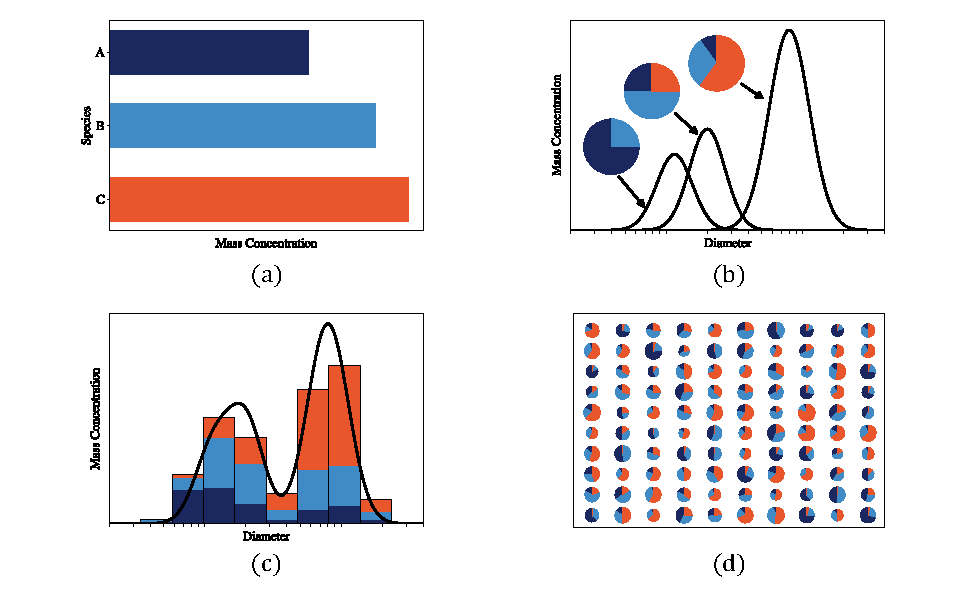
\includegraphics[width=\textwidth]{chapter1/aerosol-model-treatments.pdf}
	\caption{Illustrations of aerosol modeling treatments, each for the same aerosol population. The following representations are shown: (a) Bulk, (b) Modal, (c) 1-D sectional, (d) Particle-resolved.}
	\label{fig:aerosol-models}
\end{figure}

Thus we may consider an aerosol modeling hierarchy organized from aerosol model treatments with low complexity and computational cost to treatments that possess high complexity and representability alongside increased computational expense. Figure \ref{fig:aerosol-models} shows a series of four aerosol model treatments from across the aerosol modeling hierarchy with low complexity models in the top left and high complexity models in the bottom right. For each subfigure, the model treatment represents the same underlying aerosol population composed of three general species A, B, and C. Moving through this Figure \ref{fig:aerosol-models} sequentially, (a) corresponds to a bulk aerosol model in which only the bulk composition of the population is tracked. The aerosol population is not size-resolved, meaning that the population is monodisperse with a single prescribed particle diameter. Bulk models are the simplest aerosol treatment and require low computational cost. 

Figure \ref{fig:aerosol-models} subfigure (b) shows a modal aerosol treatment. In a modal model, the aerosol population is size-resolved and numerous lognormal distributions (``modes") are used to represent the size distribution. Within each mode, the aerosol composition is the same (i.e., the particles are internally mixed within a mode) and across modes the composition can differ (the aerosol particles are externally mixed across modes). Therefore, the compositional complexity of a modal model is tied to the number of modes represented by the model. The example shown illustrates a three-mode model, which is a common configuration for modal aerosol models. A thorough listing of modal models ranging in configuration from three to 16 modes is provided in \cite{riemer_aerosol_2019} Table 5. Note that because modal models must maintain lognormal distribution shapes, this introduces structural uncertainty in the representation of aerosols as the size distribution is artificially altered to ensure lognormal distributions. As discussed previously, this limitation of modal models helped to explain discrepancies found by \cite{crippa_impact_2017} between satellite observed AOD and modeled values.  

Moving to higher aerosol model complexity, Figure \ref{fig:aerosol-models} subfigure (c) shows a sectional aerosol treatment. Sectional models represent the aerosol size distribution using a series of adjacent bins (``sections"). Similar to the modal aerosol treatment, the composition of particles within each bin is the same while the composition is allowed to vary across bins. The example sectional treatment illustrates a 1-D sectional model with eight bins. Higher dimensional sectional models exist such as 2-D and 3-D representations whereby the additional dimension(s) is used to represent additional aerosol properties (e.g., the 3-D sectional framework of \cite{ching_three-dimensional_2016} adds dimensions for BC mass fraction and hygroscopicity).

Lastly, Figure \ref{fig:aerosol-models} subfigure (d) shows a representation of a particle-resolved model. Among the aerosol modeling hierarchy, particle-resolved models possess the highest degree of compositional complexity and representability due to the direct representation of aerosol particles via a set of computational particles. The size and composition of each particle is allowed to vary and evolution of the aerosol state is tracked by solving the general dynamic equation describing processes (e.g., transport, coagulation, condensation, emission, deposition, nucleation) that alter and age the aerosol population. In a particle-resolved model, computational particles are represented by an $A$ dimensional vector $\vec{\mu^i}\in \mathbb{R}^A$ where $A$ is equal to the number of aerosol species and the vector magnitude along each dimension $\vec{\mu_a^i}$ corresponds to the mass of species $a$ in computational particle $i$ for $a=1,...,A$ and $i=1,...,N_p$. Changes to aerosol composition due to gas-particle partitioning directly alter the computational particle vector $\vec{\mu^i}$. Processes including coagulation, deposition, and dilution are treated in a stochastic manner building off the Monte Carlo algorithm for stochastic collision-coalescence of cloud drops developed by \cite{gillespie_exact_1975}. While particle-resolved models represent individual computational particles, it is customary to assign each particle a weighting (i.e., a multiplicity factor) in order for the set of computational particles to accurately resemble the number concentration of typical aerosol populations. This is because the number of particles per unit volume can be quite high and representing each individual particle would be computationally prohibitive as the numerical cost of particle-resolved models tends to scale with the number of computational particles. 

Examples of particle-resolved models include the Particle Monte Carlo model (PartMC) (\cite{riemer_simulating_2009}). PartMC is a box model, meaning that the relative position of particles within a grid cell are not tracked. PartMC has been used to describe the complex mixing state (i.e., the compositional diversity within and across aerosols) of particles containing BC and their aging alongside quantification of the processes that contribute to aging (\cite{riemer_simulating_2009}). This represents a key advantage of particle-resolved models over coarser-resolved aerosol treatments, as the full complexity of the aerosol compositional diversity and the processes contributing to aging can be measured in a manner not possible with coarser-resolved aerosol models. Furthermore, particle-resolved models have been used to quantify error in coarser aerosol models regarding the prediction of climate-relevant aerosol properties including CCN activity and optical properties. \cite{zaveri_particle-resolved_2010} developed a ``composition-averaging" post-processing technique for averaging the compositional diversity of particle-resolved output to match that of coarser-grained aerosol models such as sectional treatments. The authors found that when the aerosol population composition was averaged to match that of a 10-bin sectional model, the resulting CCN concentrations were overestimated in the sectional treatment by up to 125\%. This illustrates the large degree of structural uncertainty present in coarser-resolved aerosol models regarding the representation of CCN activity. \cite{fierce_quantifying_2024} directly quantified this structural uncertainty between particle-resolved and modal estimates of CCN activity by comparing PartMC with the four-mode MAM4 model. The authors found that CCN activity diverged between the two models after a couple of hours and that conditions with rapid aging such as in polluted regions with a high rate of coagulation and gas-particle partitioning amplified the model disagreement. 

\subsection{Coupled aerosol-transport models}
Models which jointly represent aerosols, their aging, transport, and feedbacks on the environment alongside broader-scale atmospheric dynamics are typically a coupled system of models, one responsible for the aerosol representation as previously discussed and another model which handles atmospheric transport and evolution of meteorological variables. Global and regional scale models typically represent transport via Reynolds-averaged Navier-Stokes which models the mean flow and fully parameterizes turbulent transport. Current generation climate models represent aerosols with a modal or sectional treatment. For instance, the U.S. Department of Energy's Energy Exascale Earth System Model (E3SM) uses the 4-mode MAM4 model (\cite{golaz_doe_2022}) while the National Center for Atmospheric Research has developed the Community Earth System Model (CESM) to utilize a 40-bin sectional aerosol treatment (\cite{tilmes_description_2023}). As discussed previously, the spatial heterogeneity of emissions and other atmospheric constituents vary on scales smaller than the resolution of large scale models and thus turbulence-chemistry interactions and the impacts of chemical segregation between reactive compounds is not resolved. Joining these considerations with the impact of aerosol modeling treatment on the representation on aerosol properties such as CCN activity, there exists a need for high resolution models which utilize detailed aerosol treatments coupled with transport schemes which explicitly resolve both steady mean state and turbulent flow.

Recently, turbulence-resolving models such as UCLALES-SALSA (\cite{tonttila_uclalessalsa_2017}) and the Dutch Atmospheric Large Eddy Simulation (DALES) model (\cite{de_bruine_explicit_2019}) have coupled LES transport schemes along aerosol model treatments. Both models have been used to investigate aerosol-cloud interactions and compare model outputs against field campaign measurements. Although these models have high-resolution transport schemes, they each possess relatively coarse-resolution aerosol treatments. For instance, UCLALES-SALSA uses a 10-bin sectional treatment while DALES implements a modified version of the seven-mode M7 model to allow two additional hydrometeor modes. To our knowledge, no modeling framework has yet to leverage a high-resolution particle resolved aerosol treatment alongside turbulence resolving transport models such as LES. 

\section{Objectives of this thesis}

Past research has established a clear link between the spatial heterogeneity of both gas phase and aerosol emissions, the processes by which the aerosol age, and their resulting climate-relevant properties including CCN activity which contribute to indirect radiative forcing. Simultaneously, there exists large uncertainty in the radiative forcing due to aerosols which results in part from the coarse representation of both aerosols and their transport in global scale models and their coupling with non-linear processes that occur at the sub-grid scale such as coagulation and turbulence-chemistry interactions. Past research has led to the development of detailed aerosol model treatments and transport representations, however there has yet to be a direct coupling between particle-resolved aerosol models and turbulence-resolving transport models for use in quantifying the effects of emissions spatial heterogeneity on the aerosol state and CCN activity. 

This thesis aims to address this gap in the literature by conducting a series of first-of-a-kind simulations using the coupled model WRF-PartMC-LES which allows particle-resolved large eddy simulations. The impacts of emissions spatial heterogeneity on the aerosol state including CCN activity are investigated by quantifying changes to aerosol size, number concentration, mass fraction, and hygroscopic properties across a variety of emissions scenarios. This thesis serves to answer the following scientific questions:
\begin{itemize}
\item What is the effect of emissions spatial heterogeneity on aerosol processes (e.g., coagulation, gas-particle paritioning)?
\item As emissions spatial heterogeneity alters the aerosol processes that occur, how does this change the aerosol properties (e.g., composition, concentration, hygroscopicity) and resulting CCN activity? 
\item How is the impact of spatial heterogeneity on aerosols modulated by changes to the composition of emissions?
\end{itemize}

In addition to the primary goals of this thesis, the development of a coupled particle-resolved large eddy simulation modeling framework presents a valuable benchmark against which the representation of aerosols in coarser-resolved models (either in transport treatment or aerosol treatment) can be compared.

\begin{figure}[!t]
	\centering
	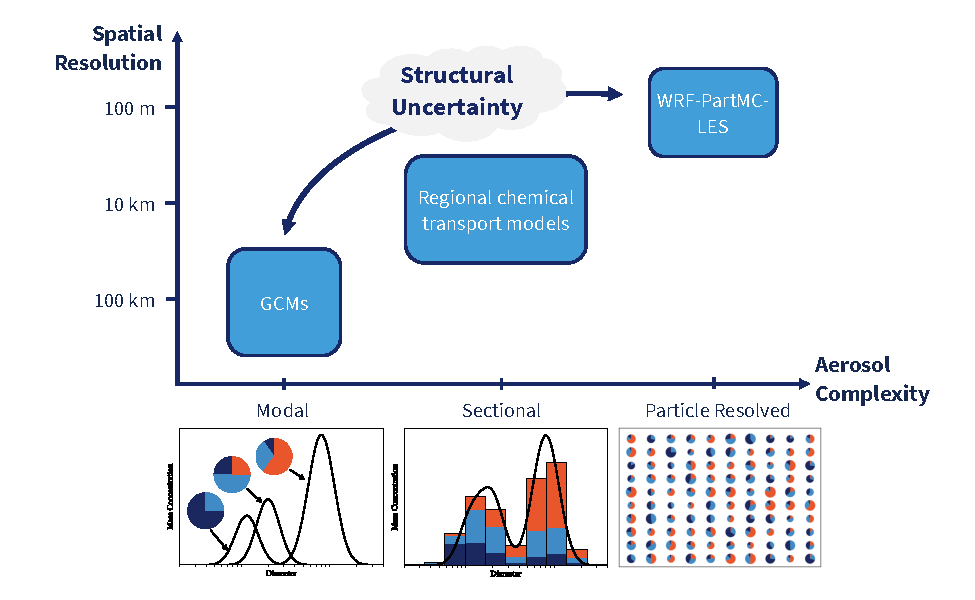
\includegraphics[width=\textwidth]{chapter1/Transport-vs-aerosol-model-struc-uncert.pdf}
	\caption{Use of WRF-PartMC-LES as a benchmark against coarser resolved aerosol-transport models for quantifying structural uncertainty in aerosol properties.}
	\label{fig:transport-vs-aerosol-model}
\end{figure} 

To illustrate this future role for WRF-PartMC-LES, Figure \ref{fig:transport-vs-aerosol-model} shows a representation of models in a coupled aerosol-transport model hierarchy. Models closer to the top right have high resolution in both space and aerosol treatment (here the spatial resolution is treated as a proxy for transport as higher resolution allows explicit depiction of turbulent transport scales). WRF-PartMC-LES serves as a benchmark against which coarser resolved models such as GCMs and regional scale models are evaluated. Structural uncertainty in key climate-relevant aerosol properties including CCN activity and aerosol optical properties could be quantified in a self-consistent manner, thereby improving understanding of uncertainty in direct and indirect radiative forcing due to aerosols.   



% !TEX root = ./main.tex
\chapter{Quantifying emissions spatial heterogeneity and mixing}
%\chapter{Quantifying emissions spatial heterogeneity, its contribution to atmospheric processes, and modeling parameterizations}

This chapter provides an overview of spatial heterogeneity (SH) and its relevance to quantifying the spatial variability of atmospheric emissions. We begin with a brief discussion of cross-disciplinary efforts to quantify SH. We then narrow our focus to quantifying the heterogeneity and mixing of reactive compounds in the atmosphere and characterize the gap in existing approaches that necessitate the development of a new, generally applicable SH metric that we will use in this thesis. The remainder of this chapter is dedicated to discussing our novel SH metric, the development of a Monte-Carlo based method for efficiently computing the metric over large domains, and its application to measuring the SH of idealized 2D patterns.  

\section{Existing Approaches to Quantifying Spatial Heterogeneity}\label{existing-sh-metrics}
SH is ubiquitous across the natural sciences ranging from ecology to atmospheric sciences. SH plays an important role in biological diversity, human land use and associated environmental feedbacks, and drives changes in atmospheric dynamics through spatially varying surface fluxes of heat, water vapor, and emissions. Despite its importance, quantifying SH is challenging in part because its definition can be highly dependent on the end use case. For instance, a metric used in geostatistics for measuring geographic variability in land use may not be particularly useful to an ecologist concerned with how spatially dependent a species population is on surrounding resources. Furthermore, mathematical assumptions central to the choice of metric such as scale similarity may not be applicable across use cases and thus limit the metrics' applicability. This has prompted the development of numerous metrics across disciplines that quantify SH. Here, we discuss various prominent SH metrics that range in applicability and complexity, and point to limitations in these approaches for use in quantifying emissions spatial heterogeneity. 

\subsection{Spatial autocorrelation and semivariograms}
Spatial correlation between measurements can be evaluated using correlograms and semivariograms. Correlograms are created by computing the correlation, measured via Pearson’s correlation coefficient, between two measurements separated by a given distance. Once the correlation across all distances and associated measurement pairs is computed, correlation is plotted against distance. A similar approach is employed for semivariograms, where the variance is plotted against distance between measurement pairs. \cite{cooper_quantifying_1997} apply these techniques to determine the spatial correlation in streams between snail density and algal biomass, which serves as an important microhabitat. The authors show how these metrics can be leveraged to quantify the spatial correlation and variability between measurements. While correlograms and semivariograms are useful for explaining the correlation and variance between spatially distributed measurements, they do not provide a one-point statistical measure of how spatially heterogeneous a region is, nor do they provide information on how variance for a quantity of interest is spatially arranged over a region.

\subsection{Fractal dimensions}
 A Fractal dimension, or fractional dimension, is a non-integer dimension (\hl{Mandelbrot 1967, 1982}). Surfaces with greater complexity across spatial scales have higher fractal dimensions and vice versa. Fractal dimensions are scale invariant, meaning that it can be used to evaluate heterogeneity across surfaces of varying area. \cite{loke_measuring_2022} discuss their use in ecology and point to numerous important limitations and considerations when utilizing fractal dimensions. The authors note that in practice, measuring fractal dimensions is challenging due to the need to quantify the broad range of scales which may be limited by the resolution of measurement techniques. Additionally real-world objects and surfaces are not truly fractal because self-similarity breaks down at certain scales. 

\subsection{Lacunarity}
Surfaces with similar fractal dimensions can have dissimilar variations or texture (i.e., their variance can be arranged in different ways). This led Mandelbrot (\hl{1983 or 1982?}) to introduce Lacunarity as a metric for quantifing the textural variation of surfaces with similar fractal dimension. Lacunarity is related to the distribution of scales of texture in a surface. Surfaces with a broader range of texture, including large and small gaps and variations, will tend to have high lacunarity. For more homogeneous objects, the distribution of texture scales will be narrower and will result in a lower lacunarity value. \cite{dong_lacunarity_2000} provide an overview of lacunarity and its use in geography and geographic information science (GIS) applications. They note that lacunarity is often quantified using a gliding box algorithm, for which the researcher must choose the gliding box size. Importantly, changes to the gliding box size do not ensure linear scaling of the difference between lacunarity of multiple patches, meaning that, for instance, a patch may have higher lacunarity compared to other patches at small gliding box sizes but may have lower lacunarity than other patches at larger gliding box size. While this may be a useful attribute of lacunarity if one wishes to evaluate the scale dependence of spatial variability and the scales at which patches appear spatially similar or dissimilar (indeed, this is a primary use case as outlined by \cite{dong_lacunarity_2000}), gliding box size introduces an additional parameter one one must choose when quantifying spatial heterogeneity and could complicate intercomparison of lacunarity measurements.

\subsection{Information entropy based metrics}
In landscape ecology, information entropy based metrics such as Shannon’s evenness index are used to quantify the patchiness of topography that is divided among numerous land uses classes. \cite{plexida_selecting_2014} evaluate a number of metrics, including Shannon’s evenness index, for measuring the topological variability and land use of central Greece. For its use in landscape ecology, Shannon’s evenness quantifies how evenly distributed the various land use types in a region are. It is defined as Shannon’s diversity index over $N$ populations (i.e., the Shannon entropy) divided by the maximum diversity index. Shannon's eveness index is useful if evaluating a region with numerous patches that are divided into different categories; however, its use is less apparent for quantifying the spatial heterogeneity of a single scalar field.

\subsection{Nearest neighbor statistics for point-based heterogeneity}
\cite{shu_quantifying_2019} discuss nearest neighbor distance statistics for use in GIS settings to quantify the spatial heterogeneity of points and apply various metrics to example cases including the spatial distribution of crime events in a city, regional seismic activity in Yutian China, and taxi routes in Beijing China. These examples range from 2D to 4D, illustrating the multidimensional applicability of nearest-neighbor metrics. The authors present a goodness-of-fit metric based on the distribution of nearest neighbor distances called the level of heterogeneity. A normalized version of the metric is proposed to resolve issues that arise when comparing datasets with differing magnitudes due to differences in scale or intensity. The authors note that while the proposed metric is suitable for capturing point-based spatial heterogeneity, it is quite computationally expensive. It is recommended that alternative nearest-neighbor metrics evaluated alongside the proposed metric should be preferred for computationally intensive datasets. 

\subsection{Multiscale norms}
Sobolev norms have been used to quantify the mixing and transport of passive scalars in fluids (\cite{thiffeault_using_2012}). Sobolev norms act as a weighted sum of the Fourier coefficients resulting from the Fourier transform of a scalar field (i.e, the passive scalar suspended in either a fluid or the atmosphere). The multiscale nature of Sobolev norms refers to the selection of Sobolev space $H^q$ over which the norm is defined. \cite{thiffeault_using_2012} show that the choice of Sobolev norm for $q<0$ is valuable for flow mixing applications as the magnitude of the norm decays alongside the mixing of the medium.

\section{Metrics for quantifying the mixing of reactive compounds}\label{metrics-reactive-mixing}
Atmospheric constituents that undergo chemical reactions including gas phase and aerosol species are subject to both spatial and temporal constraints that determine the rate at which reactions will proceed. For instance, species must be spatially collocated for reactions to occur, and they must remain in close proximity over the timescale that a given reaction will proceed. This gives rise to two important metrics: (1) segregation intensity, which quantifies the spatial proximity of reactive species and (2) the Damköhler number, which characterizes the dominant timescales governing the reactivity of species.

\subsection{Segregation intensity}
The segregation intensity, first theorized by \cite{danckwerts_definition_1952} for use in combustion processes, is a measure of how spatially segregated or mixed two reactive species are that follow a typical second-order reaction of the form

\begin{equation}
\ce{A + B -> C}.
\end{equation}
Using Reynolds decomposition to express each species concentration as the sum of a spatial average and local deviation, $[A] = \overline{[A]} + [A]'$, $[B] = \overline{[B]} + [B]'$, such that the  chemical reaction proceeds as 
\begin{equation}
\frac{d[A]}{dt} = \frac{d[B]}{dt} = -k\left(\overline{[A]}\cdot\overline{[B]} + \overline{[A'][B']} \right).
\end{equation}
The segregation intensity is then 
\begin{equation}
I_s = \frac{\overline{[A'][B']}}{\overline{[A]}\cdot\overline{[B]}},
\end{equation}
such that the chemical reaction can be expressed as 
\begin{equation}
\frac{d[A]}{dt} = \frac{d[B]}{dt} = -k\left(\overline{[A]}\cdot\overline{[B]}\right)\left(1 + I_s \right).
\end{equation}
Thus, $I_s$ can be thought of as imposing an effective reaction rate $k^{\text{eff}} = k(1+I_s)$. When $I_s = -1$, species $A$ and $B$ are fully spatially separated, such that no reaction occurs. As $I_s$ approaches zero, the two species become fully mixed and the effective reaction rate matches the ideal rate of reaction. $I_s$ can also be positive, corresponding to positive covariance between species which effectively increases the rate of reaction.

\subsection{Damköhler number}
The Damköhler number (\cite{damkohler_effect_1947}) relates the turbulence and chemical reaction timescales via the ratio
\begin{equation}
D_a = \frac{\tau_{\text{turb}}}{\tau_{\text{chem}}}.
\end{equation}
%where $\tau_{\text{turb}} = $ and $\tau_{\text{chem}} = $
The definition of turbulent and chemical timescales varies by application. For the convective boundary layer, \cite{vinuesa_fluxes_2003} adopt the following expression for the Damköhler number,
\begin{equation}
D_a = \frac{z_i}{w_*}k[B],
\end{equation}
where $w_*$ is the velocity scale in the convective boundary layer and is defined as $\left[(g/\Theta_v)\overline{w\theta}_0 z_i\right]^{1/3}$, and where $g$ is gravitational acceleration, $\Theta_v$ is virtual potential temperature, $\overline{w\theta}_0$ is vertical heat flux, and $z_i$ is the boundary layer height.

\begin{figure}[h]
	\centering
	\includegraphics[width=\textwidth]{damkohler_number_figure.pdf}
	\caption{Dependence of the Damköhler number on turbulent and reactive timescales. Figure adapted from \hl{V. Rao Kotamarthi and Yan Feng, Argonne presentation, STM meeting 2017}.}
	\label{fig:damkohler}
\end{figure}

Figure \ref{fig:damkohler} displays the three primary regimes for the Damköhler number that determine the abundance of precursor concentrations $[A]$ and $[B]$. When the turbulent and chemical timescales are balanced, $D_a = 1$. If the chemical reaction timescale is shorter than the turbulence timescale, $D_a >1$ and the concentration of the precursors will be determined by the rate at which turbulence mixes the reactive compounds (fast-chemistry regime). Conversely, if the chemical reaction timescale is slower than the turbulent timescale, $D_a<1$ such that the concentration of precursors is determined by the rate of chemical reaction (slow-chemistry regime). Thus, the Damköhler number indicates the relative importance of turbulence in chemical reactions -- in the fast chemistry regime with  reactions with $D_a > 1$, turbulent scales responsible for mixing the reactive compounds should be fully resolved. Examples of relevant gas-phase reactions in convective boundary layer that correspond to the fast-chemistry regime include oxidation of volatile organic compounds such as isoprene by OH \hl{I assume oxidation of SO2 by OH as well?}.

\section{A novel approach to quantifying spatial heterogeneity}
Existing approaches to quantifying spatial heterogeneity discussed in Section \ref{existing-sh-metrics} and metrics for mixing of reactive compounds in Section \ref{metrics-reactive-mixing} provide valuable information on the state of a heterogeneously distributed field, however each metric varies in terms of range of applicability, interpretability, and ease of implementation. 

For instance, spatial autocorrelation and semivariograms are relatively easy to interpret and are computationally efficient to measure, but they are primarily useful for capturing the correlation and variability at a single point rather than over an entire region. Alternatively, the nearest neighbor metric proposed by \cite{shu_quantifying_2019} is useful across a broad range of applications as illustrated by the authors, however, their approach is computationally expensive and is not readily interpretable to the same manner as other spatial heterogeneity metrics. Metrics for mixing provide useful information on how spatially colocated reactive compounds are and the relevant timescales that determine the abundance of precursors, however they do not provide information on how the variance in the spatial distribution of each compound is arranged. 

Thus, there exists the need for a novel spatial heterogeneity metric for use in atmospheric science applications including quantifying emissions spatial heterogeneity and subsequent atmospheric field heterogeneity once compounds are emitted into the planetary boundary layer. \hl{Mohebalhojeh et al. 2024 (in prep)} have developed a new approach to measuring spatial heterogeneity with key benefits being that their approach is broadly applicable, straightforward to interpret, and computationally efficient to measure using a Monte Carlo approach discussed in Section \ref{sh-metric-calculation}.

\subsection{Metric definition}
The spatial heterogeneity metric, subsequently $SH$, quantifies the level of heterogeneity for single scalar quantity over a 2-dimensional surface. In this thesis, the scalar of interest is either gas phase or aerosol species and the 2-dimensional surface is either the ground level in the case of emissions or a horizontal plane through the computational domain to quantify atmospheric field heterogeneity within the planetary boundary layer.

$SH$ is calculated by summing up the absolute difference between the mean of a scalar quantity over a rectangular subset of the domain and the domain averaged value for all possible subsets. Over a discrete 2-dimensional grid with $N$ cells along the x-axis and $M$ along the y-axis, there exist \\$P=(N(N-1)+1)(M(M-1)+1)$ total possible rectangular subsets. For a scalar field $f$ defined over some domain $S$, $SH$ is computed as

\begin{equation}
SH(f, S) = \frac{1}{P}\sum_{\tilde{S}\in \mathbb{R}}|\overline{f}(S) - \overline{f}(\tilde{S})|.
\end{equation}

\begin{figure}[h]
	\centering
	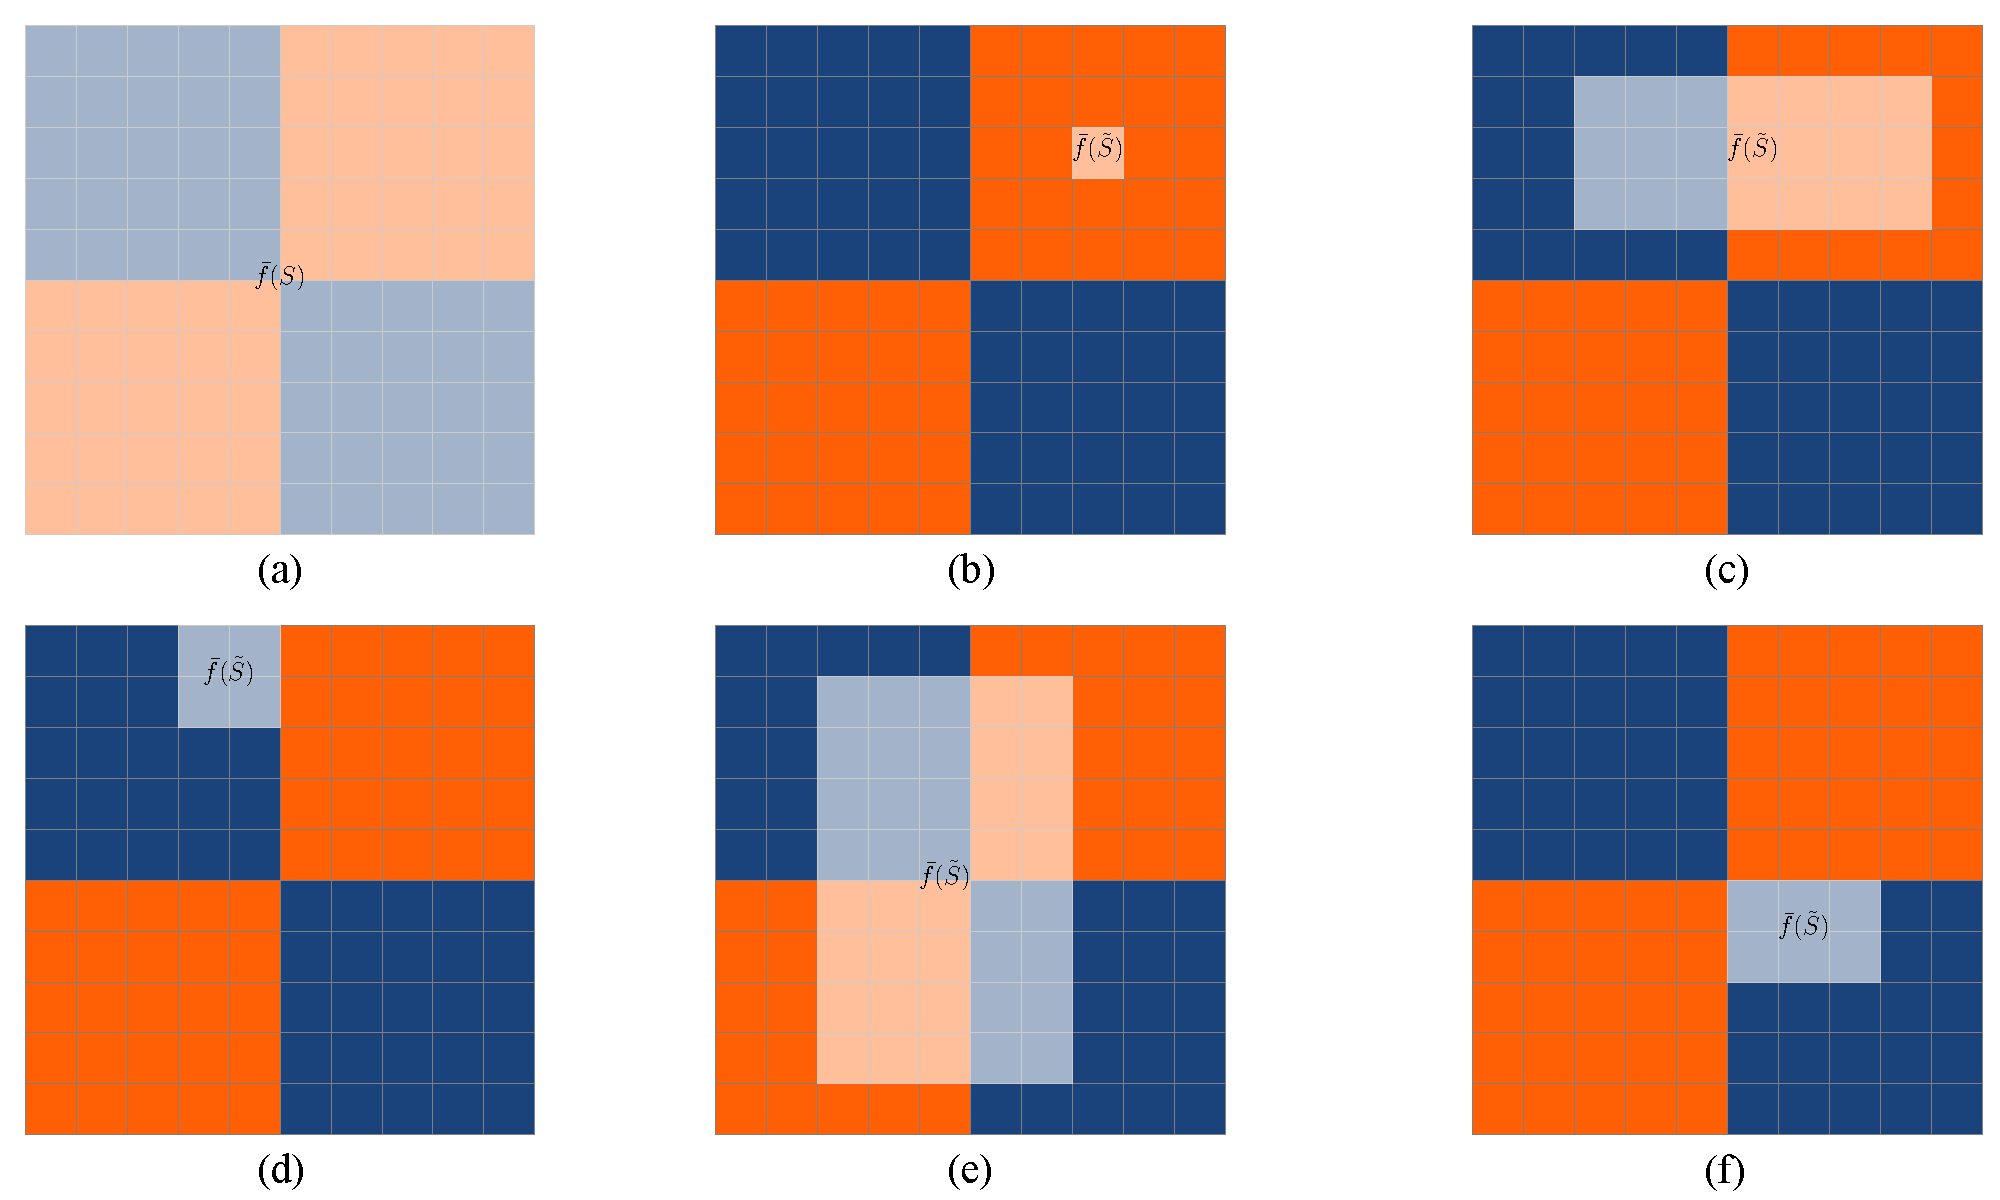
\includegraphics[width=\textwidth]{SH-subarray-examples.pdf}
	\caption{Example subsets for $SH$ calculation. (a) Full domain mean. (b-f) Examples of rectangular subsets (highlighted regions) over which the subset mean is computed.}
	\label{fig:sh-subarrays}
\end{figure}

Because the range of gas phase and aerosol emissions varies across orders of magnitude, it is useful to instead utilize a normalized version of the spatial heterogeneity metric,

\begin{equation}
SH(f, S) = \frac{1}{\overline{f}(S)\left[\frac{3}{2}(N\times M)(N-1)(M-1) + N(N-1) + M(M-1)\right]}\sum_{\tilde{S}\in \mathbb{R}}|\overline{f}(S) - \overline{f}(\tilde{S})|.
\end{equation}

A visualization of the total domain mean $\overline{f}(S)$ and domain subset means $\overline{f}(\tilde{S})$ are shown in Figure \ref{fig:sh-subarrays}. The checkerboard pattern represents an idealized emission pattern, where orange-filled cells correspond to regions of uniform emissions and dark blue regions correspond to zero emissions. $\overline{f}(S)$ is shown in subfigure (a), while five examples of rectangular subsets are displayed in subfigures (b-f).


%\subsection{Monte Carlo approach for estimating the spatial heterogeneity metric}\label{sh-metric-calculation}
\subsection{Computational methods for computing the spatial heterogeneity metric}
To calculate $SH$ over a computational domain, an array comprising the scalar quantity of interest with dimension equal to the size of the domain ($N$ by $M$) is passed to a Fortran subroutine. Here, we discuss two approaches to calculating $SH$: a computationally expensive naive looping algorithm and a significantly more efficient Monte Carlo based method.

\begin{figure}[h]
	\centering
	\includegraphics[width=\textwidth]{NSH-performance.pdf}
	\caption{Compute time for the naive looping $SH$ Fortran subroutine. The x-axis indicates the total number of domain grid cells (elements) in the array passed to the subroutine. A power law regression is plotted as the red dashed line.}
	\label{fig:nsh-performance}
\end{figure}

The naive subroutine loops over all possible rectangular subdomains which can be quite computationally expensive, especially for domains with a large number of grid cells (e.g., 100$\times$100 grid cells laterally as used for domain mesh size in this thesis). Figure \ref{fig:nsh-performance} shows the computational scaling for a Fortran subroutine using this naive looping algorithm. A power law regression (red dashed lined) is fit to the compute time vs. the total number of domain grid cells. The naive looping algorithm scales as $O(n^3)$ for $n$ the number of grid cels. For domain sizes used in this thesis ($N=M=100$), this results in a single calculation taking in excess of 2 minutes.

\begin{figure}[h]
	\centering
	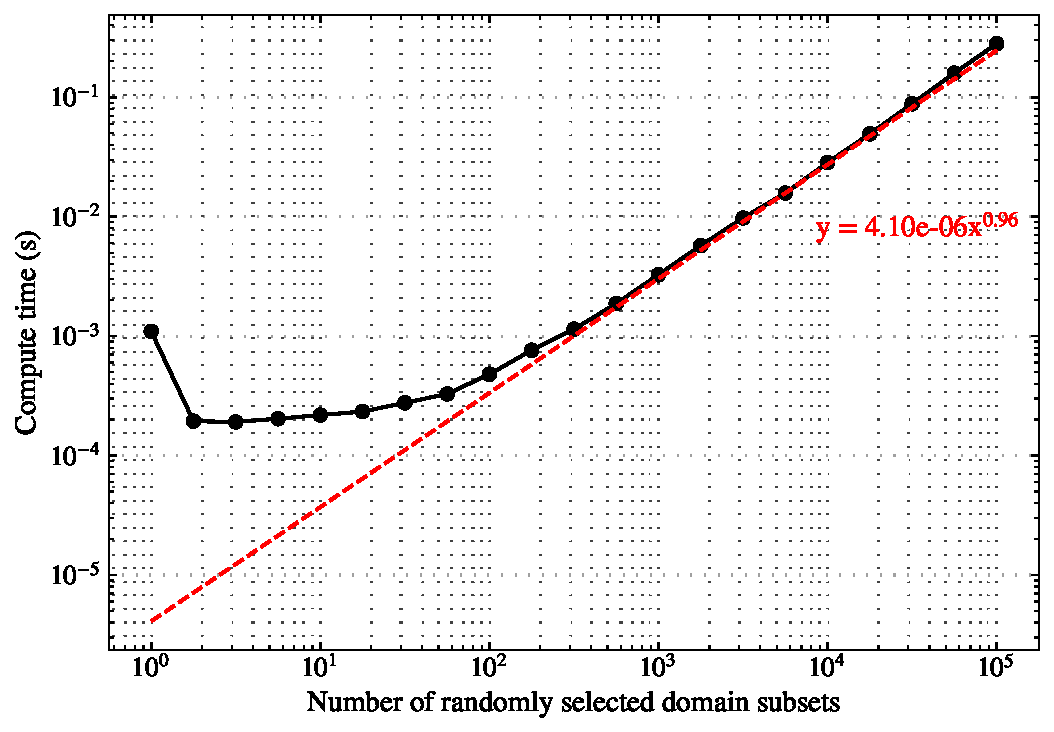
\includegraphics[width=\textwidth]{mcNSH-performance.pdf}
	\caption{Compute time for the Monte Carlo $SH$ Fortran subroutine. The x-axis indicates the number of domain subsets that are randomly selected to determine the $SH$ estimate. A power law regression is plotted as the red dashed line.}
	\label{fig:mcsh-performance}
\end{figure}

Instead of looping over every possible subdomain, we may use the fact that the probability of selecting any given subdomain is the same (i.e., the sampling probability is uniform across the entire domain) in order to construct a Monte Carlo sampling based approach for calculating $SH$. We then pass the array with domain scalar values alongside a parameter for the number of subsets to sample to our Monte Carlo-based Fortran subroutine. Figure \ref{fig:mcsh-performance} shows the compute time for corresponding number of randomly selected domain subsets, ranging from 1 to 100,000 for a domain with dimensions $N=M=100$ and $P=(100(100-1)+1)(100(100-1)+1) = 98,029,801$ total subsets. For a low number of randomly selected subsets (number of subdomains $\lesssim 100$), the algorithm scales quite weakly, suggesting that computational overhead limits speedup in this region over the naive algorithm. As the number of subdomains increases above 100, the algorithm scales as $O(S)$ for $S\subset P$ as indicated by the power law regression.

\begin{figure}[h]
	\centering
	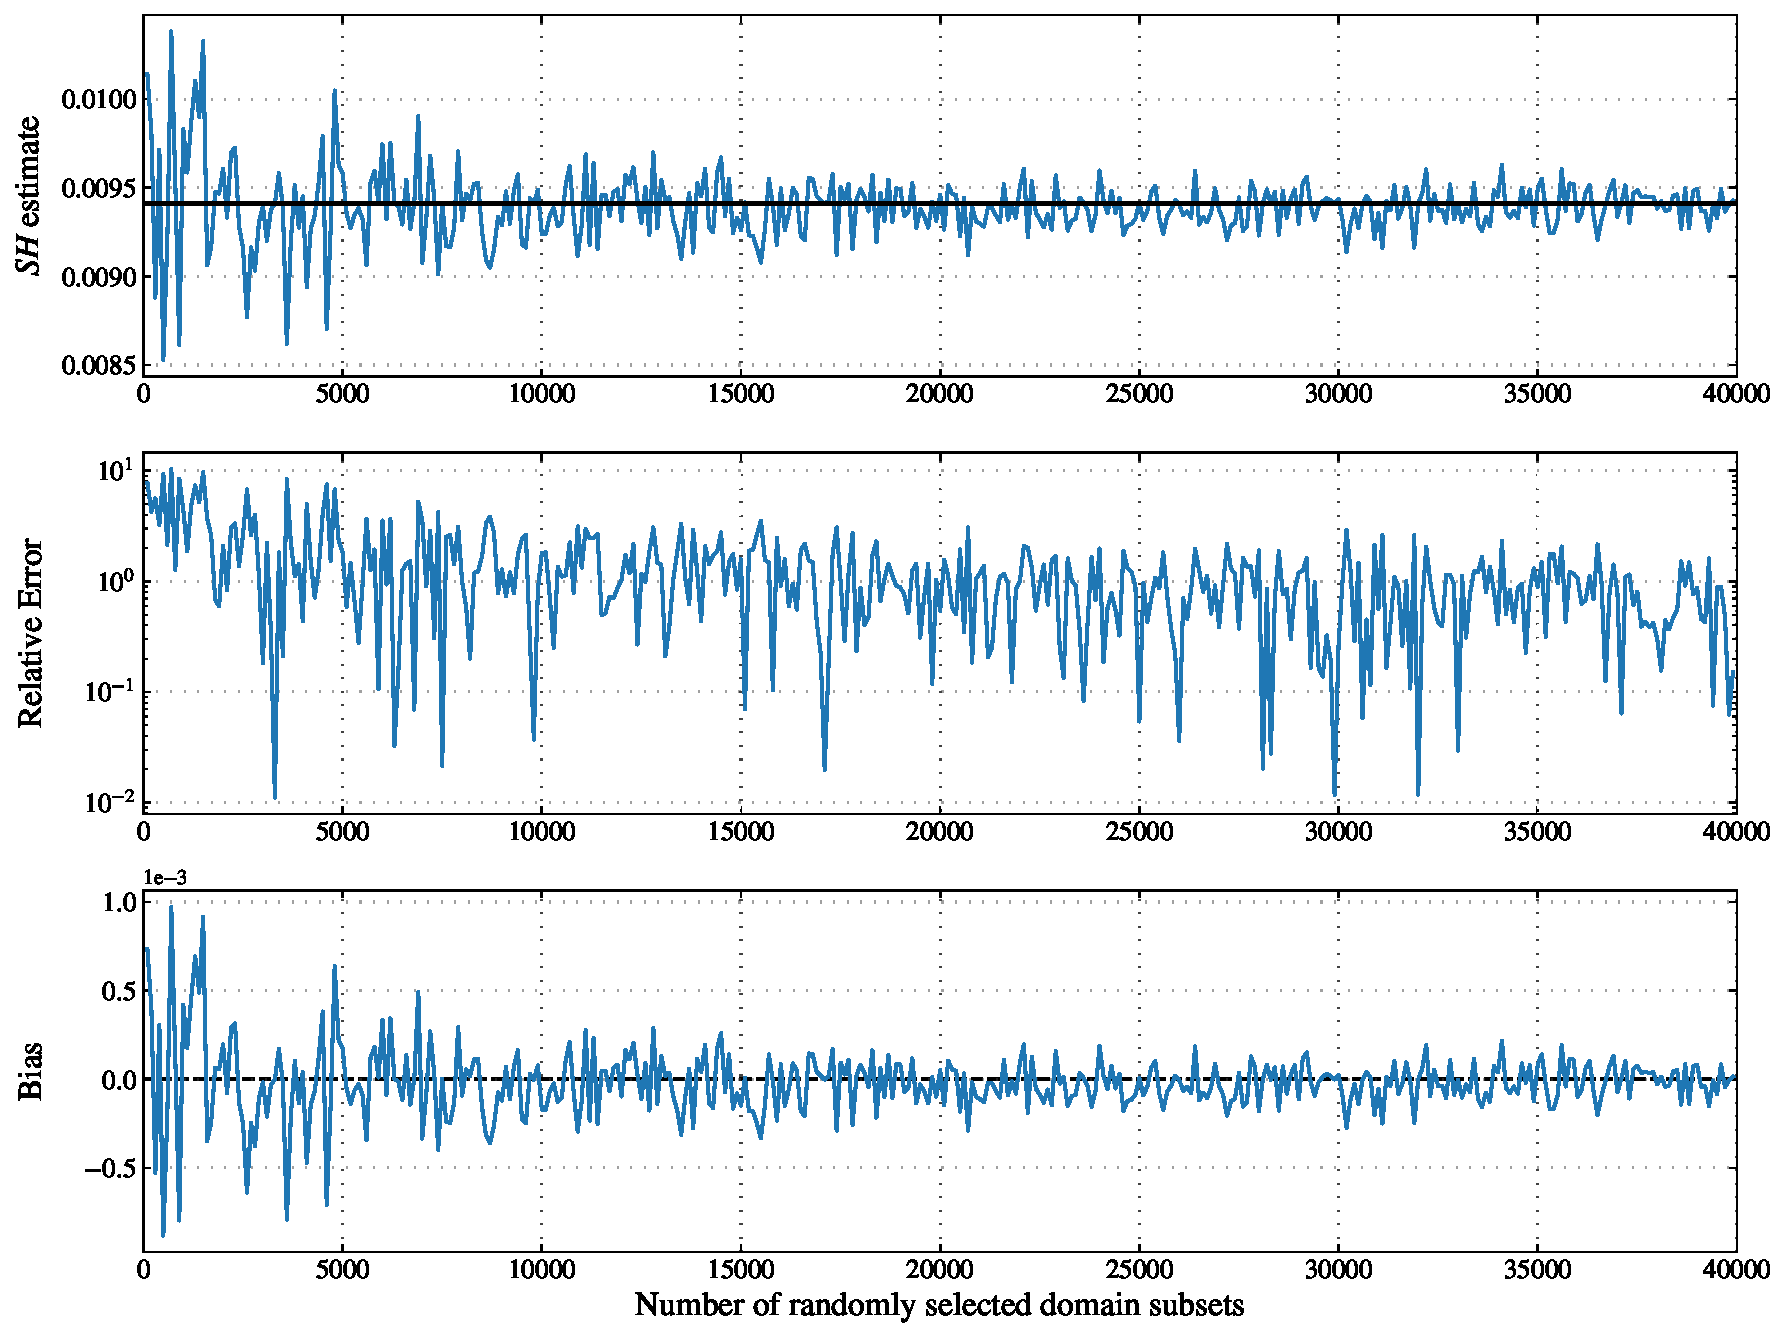
\includegraphics[width=\textwidth]{mcNSH-accuracy.pdf}
	\caption{$SH$ estimate in blue for the Monte Carlo sampling subroutine vs. the number of randomly selected domain subsets (top panel). The true value of $SH$ computed via the naive algorithm is shown as the black line.  Absolute relative error between $SH$ estimate and the true value of $SH$ (middle panel). Bias between $SH$ estimate and the true value of $SH$ (bottom panel) }
	\label{fig:mcsh-accuracy}
\end{figure}

We validate the accuracy of the Monte Carlo sampling subroutine against the naive looping approach in Figure \ref{fig:mcsh-accuracy}. First, the precise value of $SH$ was computed via the naive algorithm for a scalar field of random noise with dimensions $N=M=100$. We then vary the number of randomly selected subsets used to compute the estimate of $SH$ in the Monte-Carlo subroutine. The top panel in Figure \ref{fig:mcsh-accuracy} shows how the $SH$ estimate converges on the precise value of $SH$ (shown as a black line). The middle panel displays the relative error between $SH$ estimates and the precise value (note the logarithmic scaling). Relative error appears to plateau around $\sim1\%$ as the number of randomly selected domain subsets approaches 40,000. This suggests diminishing returns for accuracy at the expense of computational cost as discussed previously for Figure \ref{fig:mcsh-performance}. Bias between $SH$ estimates and the precise value of $SH$ is shown in the bottom panel. 

Given the performance of the Monte Carlo sampling subroutine over the naive looping approach and its ability to reach a high level of accuracy with minimal error when sampling a sufficient number of domain subsets, we utilize the Monte Carlo method for subsequent $SH$ calculations. For such calculations, we choose the number of randomly selected domain subsets to be 40,000 as this results in relative error $\lesssim 1\%$ for the domain size $N=M=100$ used in this thesis.

\subsection{Example calculations for emission patterns}


% !TEX root = ./main.tex
\chapter{Modeling tools}
This chapter discusses the modeling tools necessary for conducting simulations presented in this thesis. A description of the transport treatment, large-eddy simulations, is provided alongside discussion of requisite sub-grid scale parameterizations that we utilize. Attributes of the computational domain, including its spatial extent, grid resolution, and other defining qualities are presented. Meteorological initial conditions for simulations are discussed as well as determination of necessary spin-up time for the development of convective boundary layer in the computational domain. Subsequently, chemical mechanisms used for gas phase and aerosol chemistry are discussed. Lastly, the aerosol model, PartMC, and its coupling with the chosen transport model is discussed. 

\section{Large-eddy simulations}
Within the planetary boundary layer, turbulent eddies are responsible for mixing and transporting gases and aerosol particles as well as thermal and kinetic energy. Over time, these eddies break down due to flow instabilities, frictional losses due to interactions with physical boundaries, and the viscosity of the atmospheric constituents. Therefore, it is important for modeling frameworks that represent the planetary boundary layer to explicitly resolve the physical scales over which transport and mixing occur, as well as accurately model the dynamical tendency of kinetic energy transfer from large to small eddies. 

Representation of turbulence in modeling frameworks is a computationally challenging task because of the range of scales one must consider and the associated need for high spatial resolution. In the planetary boundary layer, turbulent eddies range in size from hundreds of meters to the Kolmogorov length scale on the order of a few millimeters \parencite{kolmogorov_local_1991}, at which size eddies break down due to kinematic viscosity of atmospheric constituents. A widespread technique when modeling the planetary boundary layer is the use of large-eddy simulations (LES). In LES, the equations of motion are filtered such that the largest, energy-containing eddies are explicitly resolved down to a grid resolution on the order of 10 meters. For eddies smaller than the resolution of the grid, sub-grid scale parameterizations are used to represent the statistical attributes of unresolved eddies, including their energy dissipation and stress forces.  

For simulation results presented in this thesis, we use the Weather Research and Forecasting model (WRF) configured for LES \parencite{skamarock_description_2008}. In practice, conducting LES studies in WRF arises from modeling choices including the representation of sub-grid scale turbulence parameterizations and adequately high grid resolution; that is, there is no ``switch" for configuring WRF in LES mode, but rather structural choices which permit representation of the relevant dynamics. 

Simulations were conducted on the University of Illinois Urbana-Champaign School of Earth, Society, and the Environment's supercomputing cluster ``Keeling". Each simulation job allocated eight of Keeling's ``J" nodes, which contain 48 cores per node for a total of 384 compute cores. Each core was allocated 5 GB of memory (the approximate maximum allocatable amount of memory per core). Wall time for simulations was approximately 74 hours.

We wish to acknowledge that simulations presented in this thesis are heavily idealized in their setup. We shall discuss numerous simplifying assumptions in detail in subsequent sections, such as the use of sub-grid scale turbulence parameterizations, the use of an idealized sounding for specifying meteorological initial conditions, the choice of a topographically smooth domain, and the absence of horizontal wind in the initial condition. In large part, these choices are to intended to resolve the relevant scale of dynamics and isolate the impacts of emissions spatial heterogeneity on the atmospheric state, including gas phase concentrations and aerosol properties. These simplifying assumptions limit the broader applicability of simulation results to more realistic settings in which there exists a complex interaction between the study region characteristics (e.g., variations in atmospheric stability, wind, and topography) and the atmospheric state; however, these simulations make possible a focused, process-level analysis of the coupling between emission spatial heterogeneity and the atmospheric state.

\subsection{Sub-grid scale parameterizations}
A key choice in the implementation of LES is the selection of sub-grid scale turbulence parameterizations. Specifically, one must parameterize the sub-grid scale stress $\tau_{ij}$ and sub-grid scale fluxes $q_i$. The stress tensor $\tau_{ij}$ represents the deformational forces acting both normal ($i=j$) and perpendicular ($i\neq j$) to each grid cell, while the sub-grid scale fluxes $q_i$ refers to the transport of scalars such as momentum, heat, or other quantities by unresolved eddies. A common technique for the closure of sub-grid scale stress and flux is the use of eddy-viscosity models. This technique was pioneered by Smagorinsky for parameterizing the motion of sub-grid scale eddies in a model of general circulation \parencite{smagorinsky_general_1963}. Eddy-viscosity models mimic the linear relationship between the stress tensor of a Newtonian fluid and shearing forces acting on the fluid scaled by the fluid's molecular viscosity. As such, eddy-viscosity models are not fundamentally grounded in physical tendencies of turbulent flows, but rather provide an empirical approximation that mimics Newtonian fluids and has been shown to be reasonable for representing sub-grid scale turbulence in modeling studies of the planetary boundary layer \parencite{stoll_large-eddy_2020}. The sub-grid scale stress and sub-grid scale flux are then expressed as 
\begin{align}
\tau_{ij} &= -2\nu_T \tilde{S}_{ij},\\
q_i &= -\nu_{\theta}\frac{\partial \tilde{\theta}}{\partial x_i}, 
\end{align}
where $\nu_T$ is the eddy viscosity coefficient, $\tilde{S}_{ij} = \frac{1}{2} (\partial\tilde{u_i}/\partial x_j + \partial\tilde{u_j}/\partial x_i )$ is the resolved strain rate tensor (i.e., the rate at which straining forces such as expansion and shearing due to resolved flow occur), $\nu_{\theta}$ is the eddy diffusivity coefficient for some scalar quantity $\theta$, and $\partial \tilde{\theta} / \partial x_i$ is the resolved-scale gradient of scalar $\theta$ in direction $x_i$. As $\tilde{S}_{ij}$ and $\partial \tilde{\theta} / \partial x_i$ are known quantities determined at the resolved scale, eddy-diffusivity models then become a matter of determining $\nu_T$ and $\nu_{\theta}$. 

Deardorff was the first to implement Smagorinsky's eddy-diffusivity sub-grid scale model for LES, however, he found that the model was overly diffusive for short wavelength features \parencite{deardorff_numerical_1970}. \textcite{deardorff_stratocumulus-capped_1980} instead proposed an alternative eddy-diffusivity model in which a prognostic equation for sub-grid scale kinetic energy $E$ is solved alongside expressions for $\nu_T$ and $\nu_{\theta}$
\begin{align}
\frac{\partial E}{\partial t}  &= -\frac{\partial\tilde{u_j}E}{\partial x_j} + 2\nu_T\tilde{S}_{ij}\tilde{S}_{ij} - \nu_{\theta}\frac{\partial \tilde{b}}{\partial z} + \frac{\partial}{\partial x_j}2\nu_T\frac{\partial E}{\partial x_j} - \epsilon, \\
\nu_T &= C_1\ell\sqrt{E}, \\ 
\nu_{\theta} &= \left(1 + 2 \frac{\ell}{\Delta}\right)\nu_T,
\end{align}
where $b$ is buoyancy, $\epsilon$ is the turbulent kinetic energy (TKE) dissipation, $C_1$ is a coefficient that must be specified by the modeler, and $\ell$ is the turbulent length scale. In this thesis, we use Deardorff's TKE scheme for eddy diffusivity. Customarily, $C_1 = 0.1$ and we use this value as recommended by an idealized test case for LES simulations packaged alongside the WRF codebase.

% Some stuff about Smagorinsky's eddy diffusivity model that I don't think pertains to my simulations
\iffalse

Smagorinksy showed that the sub-grid scale stress can be represented as the following 
\begin{equation}
	\tau_{ij} = -2\left(C_S\Delta\right)^2 |\tilde{S}| \tilde{S}_{ij},
\label{equation:smagorinsky_sgs_stress}
\end{equation}
where $C_S$ is the Smagorinsky constant that must be specified by the modeler, $\Delta = (\Delta_x \Delta_y \Delta_z)^{1/3}$ is the geometric mean length scale for spatial discretization in a 3D domain, $|\tilde{S}| =\sqrt{2\tilde{S}_{ij}\tilde{S}_{ij}}$ is the magnitude of the resolved strain rate, and $\tilde{S}_{ij} = \frac{1}{2} (\partial\tilde{u_i}/\partial x_j + \partial\tilde{u_j}/\partial x_i )$ is the resolved strain rate tensor (i.e., the rate at which straining forces such as expansion and shearing due to resolved flow occur). The Smagorinsky constant takes values typically in the range of 0.10--0.20. In WRF-LES, we use a value of $C_S = 0.18$ as recommended by an idealized test case for LES simulations packaged alongside the WRF codebase.
\begin{table}[h!]
\centering
\begin{tabular}{||c c||} 
 \hline
 Sub-grid scale Parameter & Value\\ [0.5ex] 
 \hline\hline
 $C_s$ & 0.18 \\ 
 $C_k$ & 0.1 \\ [1ex] 
 \hline
\end{tabular}
\caption{Table with sub-grid scale eddy coefficients}
\label{table:1}
\end{table}

\fi


\subsection{Computational domain}
We model the planetary boundary layer in an 3D idealized domain with dimensions 10 km in both lateral dimensions and 2 km vertically. A horizontal resolution of 100 m was chosen alongside a vertical resolution of approximately 20 m\footnote{WRF uses a terrain-following pressure ``eta" coordinate system for vertical levels. Note that because the domain only extends to 2 km vertically, vertical levels are nearly equally spaced apart.}, resulting in a domain of 100x100x100 grid cells. This resolution is necessary to resolve the scales of motion responsible for turbulent transport in the planetary boundary layer. A higher resolution vertically is desired in order to accurately represent vertical motions due to convective and turbulent transport. Time discretization is set to 1 second for all simulations, however sub-models such as chemistry (when active) further refine time discretization to maintain stability for integration. 

The domain is absent of any topographic features with a uniform, flat surface. As noted previously, past work by \textcite{gustafson_jr_downscaling_2011} has shown that local flow heterogeneities due to topographical variation alters the concentration of both gas phase species and aerosol. Our use of an idealized domain absent of topography isolates the contribution of emissions spatial heterogeneity to changes in the gas phase and aerosol state. Latitude and Longitude coordinates of (0, 0) are used internally for computing the solar zenith angle necessary for photolysis calculations, however, the domain's idealized topography is not intended to match the geographic region surrounding these coordinates. Radiation is handled by the chemistry submodel which utilizes an idealized parameterization of photolysis rates based on solar zenith angle. Simulations are configured to begin at 09:00 local time and run for 6 hours through 15:00 local time on the Vernal Equinox to balance photolysis rates in the morning and afternoon. 

\subsection{Meteorological Initial Conditions}
 
 \begin{figure}[h]
	\centering
	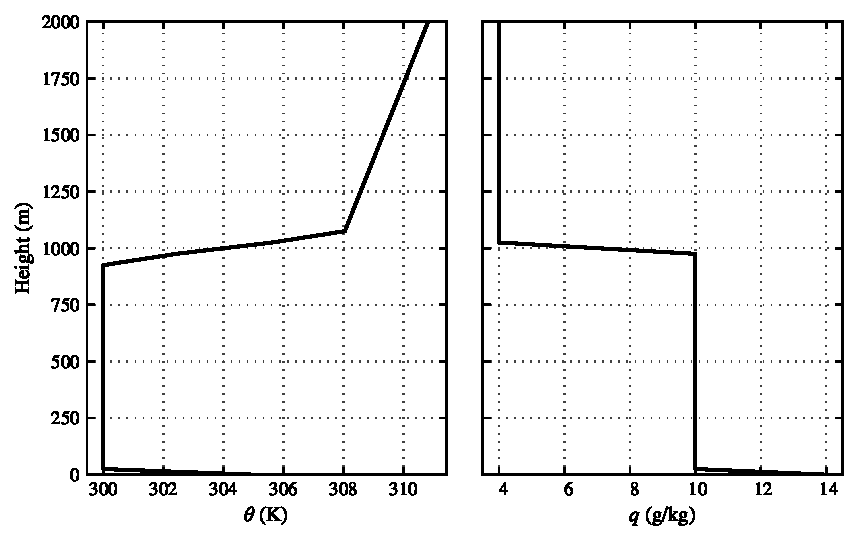
\includegraphics[width=\textwidth]{figures/chapter3/WRF-LES_default_sounding.pdf}
	\caption{Idealized atmospheric sounding used for domain meteorological initial conditions. Initial conditions for potential temperature (left) and specific humidity (right).}
	\label{fig:sounding}
\end{figure}

The domain meteorological conditions are initialized using an ideal sounding typical of a convective boundary layer (see Figure \ref{fig:sounding}). The chosen sounding is provided alongside the WRF codebase as part of a set of ideal test cases including LES of the planetary boundary layer. The lowest 25 m of the atmosphere are initially unstable to allow for parcels to rise due to buoyancy into the neutral planetary boundary layer that extends to approximately 1 km. Above this point, the planetary boundary layer is capped by an inversion up to 2 km. 

Both zonal ($u$) and meridional ($v$) wind are set to zero throughout the entire domain. \textcite{tian_how_2022} and \textcite{fast_impact_2019} both show that the impact of surface heterogeneities in surface heat fluxes on cloud formation and type are sensitive to wind conditions, and are most pronounced for minimal background winds. Extending the relevance of these findings to this thesis, our choice of an initial condition characterized by zero winds is intended to isolate the impact of emissions spatial heterogeneity on the evolving atmospheric state of gasses and aerosols.

At the surface, the specific humidity $q$ is highest at 14~\si{g.kg^{-1}} and lowers to a uniform 10~\si{g.kg^{-1}} within the planetary boundary layer. Above the planetary boundary layer, $q$ is a uniform 4~\si{g.kg^{-1}} extending vertically to the top of the domain. Simulations in this thesis do not consider cloud formation and microphysics. Note that relative humidity does not exceed 100\% at any point during simulations. Thus, in subsequent chapters, quoted CCN concentrations at specified supersaturation levels indicate the number of particles that would activate at the corresponding supersaturation in accordance with each particle’s critical supersaturation. Given the simplified radiation treatment, the surface temperature does not respond to radiative heating and radiative parameters such as surface albedo are not considered. Instead, a uniform surface heat flux of 0.24~\si{K.m.s^{-1}} is set and random perturbations of the temperature field are imposed at the lowest four levels to initiate turbulence. The surface heat flux is responsible for maintaining convection and turbulent transport over the course of the simulation. Due to uniform surface heating, we do not consider the effect of horizontal gradients in radiative heating on dynamics such as the development of secondary circulations. Boundary conditions are periodic along all lateral boundaries.

\iffalse
\begin{itemize}
\item Note the Coriolis parameter is 1e-4 which is roughly what it is at around 45 degrees lat.. this is different than the 0,0 I assume for the SZA calculations - is this passed as a value or is this calculated in the ideal initialization routine? \hl{this may actually be okay since the initial wind field is zero everywhere and turbulence and convection are the only sources of transport. The domain is also relatively small so my hunch is that the Coriolis force is insignificant. Technically I think this depends on a scale analysis using Rossby number U/lf where f is 1e-4 and U and l are the characteristic length scales for velocity and space respectively.}
\end{itemize}
\fi


\subsection{Simulation spin-up}

\begin{figure}[h]
	\centering
	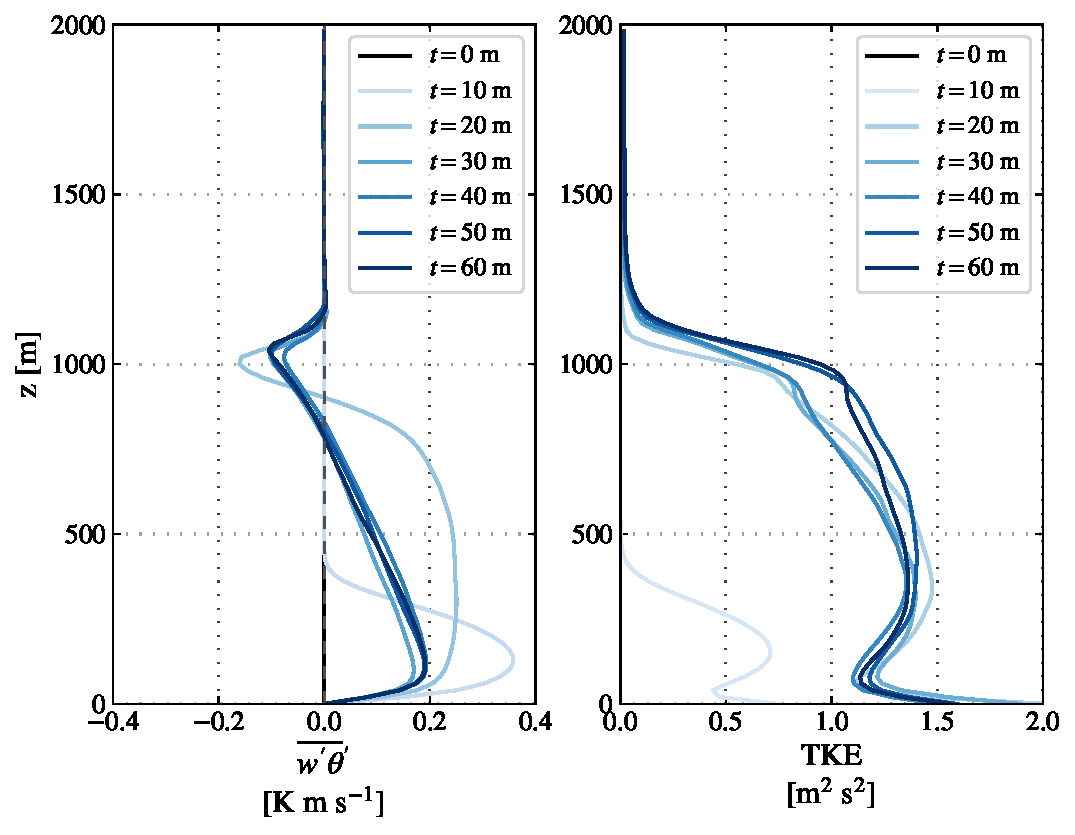
\includegraphics[width=\textwidth]{figures/chapter3/heat-flux-and-tke-profile.pdf}
	\caption{Vertical profiles of resolved-scale vertical heat flux (left) and TKE (right) at intervals of 10 minutes during the first hour of simulation spin-up. Black lines represent the initial condition, where both quantities are zero everywhere.}
	\label{fig:heat-flux}
\end{figure}

Prior to the release of gas and aerosol emissions, the simulation is allowed to spin up for a period of 1 hour. During this time, convection and turbulence within the boundary become well established and throughly mix the initial conditions for gases and aerosols alongside transporting heat and momentum. In a well established convective boundary layer, the profile of vertical heat flux should decrease approximately linearly with height. This is because eddies transport quantities down gradient. As the source of heat flux is located at the surface, the transport of potential temperature perturbations due to surface heating becomes linearly stratified. Both resolved-scale\footnote{Ideally, one would evaluate total (resolved + parameterized) vertical heat flux and total TKE. WRF does not provide output for sub-grid scale quantities, so it would be necessary for one to modify the codebase to allow exporting these additional data.} vertical heat flux and TKE profiles are shown in Figure \ref{fig:heat-flux} in increments of 10 minutes from $t=0$~minutes to $t=1$~hour. Initially, the vertical heat flux is zero everywhere due to the initial condition of zero vertical velocity. At $t=10$~minutes, the vertical heat flux is localized near the surface and exceeds 0.3~\si{K.m.s^{-1}}. By $t=30$~minutes, initial transient behavior in the vertical heat flux relaxes as the convective boundary layer becomes more well established and the heat flux profile takes on a linearly decreasing trend with height. Profiles for subsequent times agree closely with the profile at $t=30$~minutes, indicating that the convective boundary layer is near fully established by 30 minutes. Note that the TKE profiles in Figure  \ref{fig:heat-flux} indicate that energy-containing eddies in the upper boundary layer continue to develop through $t=1$~hour, as TKE increases in the upper boundary layer from $\sim 0.7$~\si{m^2.s^{-2}} at $t=30$~minutes to $\sim 1.1$~\si{m^2.s^{-2}} by $t=1$~hour. Thus 1 hour of model spin-up time was chosen to adequately allow for development of the convective boundary layer and resolved scales of turbulence.


\section{Gas phase simulations}

\subsection{Chemical mechanism}
In Chapter 4, we will evaluate the impact of emissions spatial heterogeneity on gas phase reactions with a particular focus on ozone production. We select the chemical mechanism Carbon-Bond Mechanism-Z (CBMZ) for gas phase photochemical reactions \parencite{zaveri_new_1999}. CBMZ models both inorganic and organic compounds prevalent in anthropogenic and biogenic emissions. CBMZ allows computationally efficient calculation of over 100 reactions across dozens of chemical species. This is possible due to the model's ``lumped-structure" approach to grouping similar organic compounds by their carbon bond structure (e.g, alkanes, carbonyls, etc.). This reduces the need for tracking large numbers of organic species and reactions. Despite simplifications to the organic chemistry mechanism, CBMZ has been shown to accurately represent concentrations of compounds of primary interest for atmospheric chemistry applications (e.g., O$_3$, NO$_x$, etc.) \parencite{zaveri_new_1999}. 

\subsection{Initial conditions and emissions}\label{gas-phase-ics-and-emiss}

\begin{table}[!t]
\centering
\caption{Gas phase emissions and initial conditions. Table adapted from \textcite{riemer_simulating_2009} with permission.}
\begin{tabular*}{\linewidth}{@{\extracolsep{\fill}} lccr}
\\[-2ex]\hline 
     \hline \\[-2ex] Species & Symbol & Initial Mole Fraction (ppb) & Emissions (nmol m\textsuperscript{-2} s\textsuperscript{-1}) \\
\midrule
Nitric oxide & NO & 0.1 & 31.8 \\
Nitrogen dioxide & NO\textsubscript{2} & 1.0 & 1.67 \\
Nitric acid & HNO\textsubscript{3} & 1.0 & \\
Ozone & O\textsubscript{3} & 50.0 & \\
Hydrogen peroxide & H\textsubscript{2}O\textsubscript{2} & 1.1 & \\
Carbon monoxide & CO & 21 & 291.3 \\
Sulfur dioxide & SO\textsubscript{2} & 0.8 & 2.51 \\
Ammonia & NH\textsubscript{3} & 0.5 & 6.11 \\
Hydrogen chloride & HCl & 0.7 & \\
Methane & CH\textsubscript{4} & 2200 & \\
Ethane & C\textsubscript{2}H\textsubscript{6} & 1.0 & \\
Formaldehyde & HCHO & 1.2 & 1.68 \\
Methanol & CH\textsubscript{3}OH & 0.12 & 0.28 \\
Methyl hydrogen peroxide & CH\textsubscript{3}OOH & 0.5 & \\
Acetaldehyde & ALD2 & 1.0 & 0.68 \\
Paraffin carbon & PAR & 2.0 & 96 \\
Acetone & AONE & 1.0 & 1.23 \\
Ethene & ETH & 0.2 & 7.2 \\
Terminal olefin carbons & OLET & 2.3 \(\cdot 10^{-2}\) & 2.42 \\
Internal olefin carbons & OLEI & 3.1 \(\cdot 10^{-4}\) & 2.42 \\
Toluene & TOL & 0.1 & 4.04 \\
Xylene & XYL & 0.1 & 2.41 \\
Lumped organic nitrate & ONIT & 0.1 & \\
Peroxyacetyl nitrate & PAN & 0.8 & \\
Higher organic acid & RCOOH & 0.2 & \\
Higher organic peroxide & ROOH & 2.5 \(\cdot 10^{-2}\) & \\
Isoprene & ISOP & 0.5 & 0.23 \\
Alcohols & ANOL & & 3.45 \\
\\[-2ex]\hline 
     \hline \\[-2ex]
\end{tabular*}
\label{table:gas_emiss_ics}
\end{table}

Gas phase initial conditions and emissions are chosen to represent species and concentrations typical of an urban plume and are adopted from \textcite{riemer_simulating_2009}. The authors determined gas phase concentrations and emission rates via the 1987 Southern California Air Quality Study (SCAQS) data set which contains measurements of both gas phase species and particulate matter mass concentrations collected at multiple sites across the Los Angeles basin \parencite{zaveri_model_2008}. Table \ref{table:gas_emiss_ics} contains all gas phase initial conditions and emission rates. Empty entries signify zero concentrations or emission rates. To allow for simulation spin-up, all emission rates are set zero during the first hour of simulations. Subsequently, emitted compounds are released only at the surface and at a constant rate as specified in Table \ref{table:gas_emiss_ics} for the remainder of the simulation.



\section{Multiphase simulations}
\subsection{Chemical mechanism}
Chapter 5 presents simulation results where both gas phase chemistry and aerosol processes (e.g., coagulation, gas-particle partitioning, etc.) are modeled. Both gas phase and aerosol chemistry is represented using the Model for Simulating Aerosol Interactions and Chemistry (MOSAIC) \parencite{zaveri_model_2008}. It should be noted that CBMZ is included a sub-model within MOSAIC for handling gas phase chemistry. For aerosol chemistry, MOSAIC simulates dynamic gas-particle partitioning and phase-dependent thermodynamic equilibrium. A key challenge for modeling aerosol chemistry is that the coupled system of solid-liquid phase reactions that govern aerosol thermodynamic equilibrium is often numerically stiff due to the rate of reactions varying over large timescales. Often, chemical mechanisms solve such stiff systems in a computationally expensive manner either by iterative techniques or by directly minimizing the Gibbs Free energy of the system. MOSAIC takes an alternative approach whereby the system of equilibrium reactions is reformulated as a pseudo-transient system. This recasts the system as ordinary differential equations, for which standard numerical techniques are used to integrate and obtain equilibrium steady state solutions. This approach makes MOSAIC computationally efficient while maintaining good agreement when benchmarked against numerically rigorous and accurate models \parencite{zaveri_model_2008}.


\subsection{Aerosol representation}

We use the Particle Monte Carlo (PartMC) model for particle-resolved representation of aerosols \parencite{riemer_simulating_2009}. In PartMC, aerosol particles are represented via a set of computational particles with appropriate multiplicity to represent the desired aerosol population. Each computational particle is allowed to compositionally vary due to aerosol processes (e.g., coagulation, condensation, gas-particle partitioning, etc.), thus allowing the representation of a far greater degree of compositional diversity and aerosol properties than sectional or modal based aerosol models. PartMC is a box model, meaning that within computational grid cells, the position of computational particles is not tracked. Instead, processes such as coagulation are handled in the probabilistic manner of \textcite{gillespie_exact_1975}. PartMC is coupled with MOSAIC, thereby leveraging the computational efficiency and accuracy of each model in allowing full representation of an aerosol state (number and mass concentration, per-particle composition) under aging due to both aerosol physical processes and chemical reactions.

\textcite{curtis_single-column_2017} coupled PartMC-MOSAIC with WRF for a single column model of the planetary boundary layer. The authors developed approaches for modeling the turbulent diffusion and dry deposition of aerosol particles as stochastic processes. The resulting modeling framework, WRF-PartMC-MOSAIC, is extended here for use with 3D LES. 

For WRF-PartMC-MOSAIC-LES, we use 100 computational particles per grid cell for a total of 100 million computational particles throughout the domain at initialization. This value was chosen to balance computational efficiency and storage demands alongside numerical representability---too few computational particles will result in random noise for aerosol population properties due to the stochastic nature of the PartMC model.

\subsection{Initial conditions and emissions}\label{aerosol-ics-and-emiss}

\begin{table}[!t]
\centering
\caption{Aerosol emissions and initial conditions. Table adapted from \textcite{riemer_simulating_2009} with permission.}
\begin{tabular*}{\linewidth}{@{\extracolsep{\fill}} cccccc}
\\[-2ex]\hline 
     \hline \\[-2ex] Initial/Background  & $N$ (m$^{-3}$) & $D_{\text{gn}}$ ($\mu$m) & $\sigma_g$ & Composition by Mass\\
 \midrule
Aitken Mode & $3.2 \cdot 10^9$ & 0.02 & 1.45 & 50\% (NH$_4$)$_2$SO$_4$, 50\% POA\\
Accumulation Mode & $2.9 \cdot 10^9$ & 0.116 & 1.65 & 50\% (NH$_4$)$_2$SO$_4$, 50\% POA\\
\midrule
Emissions & $E$ (m$^{-2}$ s$^{-1}$) & $D_{\text{gn}}$ ($\mu$m) & $\sigma_g$ & Composition by Mass\\
\midrule
Meat cooking & $9 \cdot 10^6$ & 0.086 & 1.9 & 100\% POA\\
Diesel vehicles & $1.6 \cdot 10^8$ & 0.05 & 1.7 & 30\% POA, 70\% BC \\
Gasoline vehicles & $5 \cdot 10^7$ & 0.05 & 1.7 & 80\% POA, 20\% BC \\
\\[-2ex]\hline 
     \hline \\[-2ex]
\end{tabular*}
\label{table:aero_emiss_ics}
\end{table}

Initial conditions and emissions of gas phase species match those discussed in Section \ref{gas-phase-ics-and-emiss} and are displayed in Table \ref{table:gas_emiss_ics}. Similarly, aerosol initial conditions and emission rates are adopted from \textcite{riemer_simulating_2009}, who based aerosol distributions, composition, and emission rates off measurements collected as part of the SCAQS campaign in the Los Angeles valley. Aerosol initial conditions and emission properties are summarized in Table \ref{table:aero_emiss_ics}. Size distributions for aerosol initial conditions and emissions are shown in Figure \ref{fig:aero_ic_dist} and Figure \ref{fig:aero_emiss_dist}, respectively. The aerosol initial condition is comprised of two modes, including a Aitken mode and accumulation mode. Each mode is an equal mixture of 50\% ammonium sulfate and 50\% primary organic aerosol (POA). Three emission modes are chosen to represent emissions from various urban combustion sources, including cooking, diesel vehicles, and gasoline vehicles. The cooking emission mode is comprised of 100\% POA and the diesel and gasoline modes are each a mixture of POA and black carbon (BC). 



\begin{figure}[!t]
  \centering
  \begin{subfigure}
    \centering
    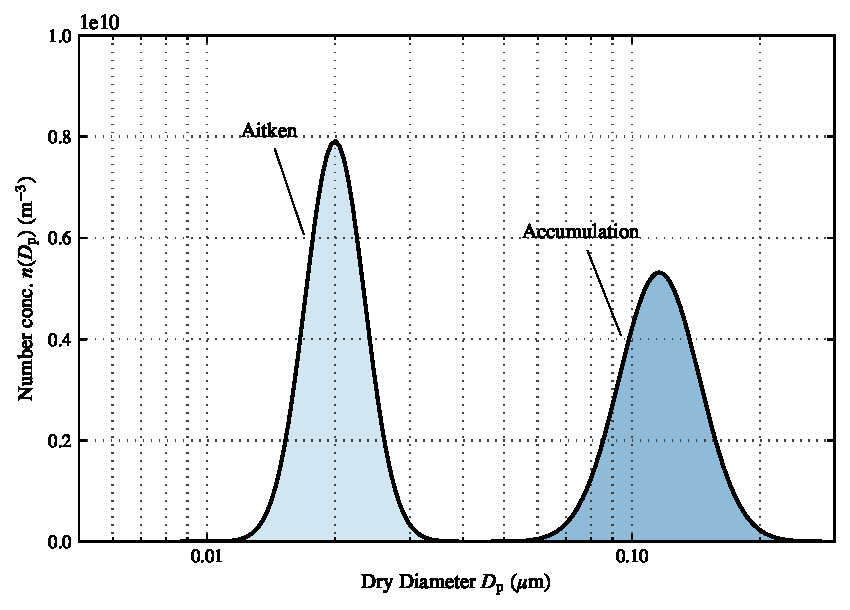
\includegraphics[width=.85\textwidth]{figures/chapter3/urban-plume-aerosol-ic.pdf}
    \caption{Aerosol initial condition size distributions.}
    \label{fig:aero_ic_dist}
  \end{subfigure}
   \vspace*{5mm} 
  \begin{subfigure}
    \centering
    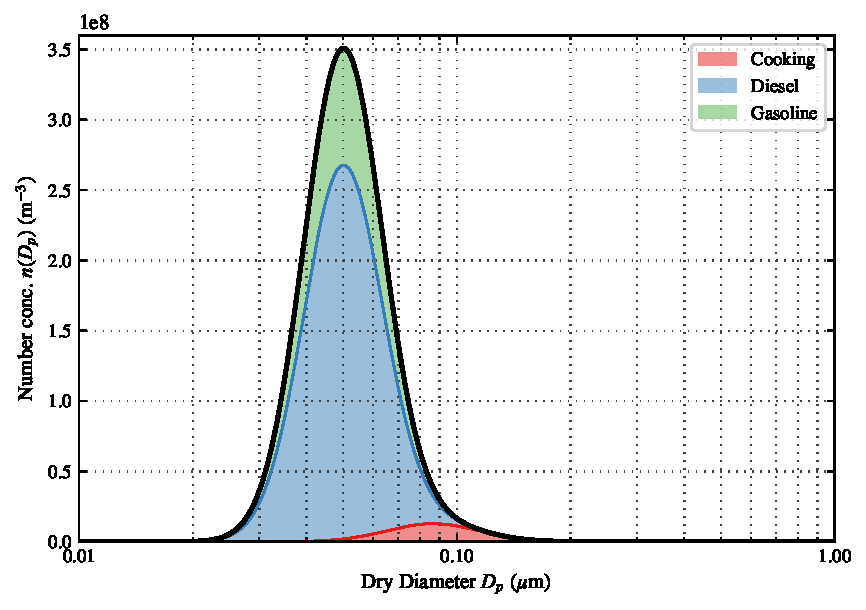
\includegraphics[width=.85\textwidth]{figures/chapter3/urban-plume-aerosol-emissions.pdf}
    \caption{Aerosol emission size distributions. The cumulative emissions number distribution is shown as the thick black line alongside individual emission modes indicated by the filled regions.}
    \label{fig:aero_emiss_dist}
  \end{subfigure}
\end{figure}




% !TEX root = ./main.tex
\chapter{Impacts of emissions spatial heterogeneity on gas-phase reactions}

This chapter investigates the impacts of gas phase emissions and associated chemical reactions on the production of ozone in the planetary boundary layer. The effect emissions spatial heterogeneity on ozone production is explored across numerous emissions scenarios with ranging emissions spatial heterogeneity. We find that for the most heterogeneous emissions case, ozone production is reduced in the mid-boundary layer by up to $\sim13\%$. We also evaluate the spatial heterogeneity of ozone and its precursor compounds NO$_x$ and volatile organic compounds (VOCs) after they are emitted. We find that $SH$ varies considerably across precursors and also exhibits spatio-temporal variability.

\section{Simulated emissions scenarios}\label{gas-emission-scenarios}

\begin{figure}[h]
	\centering
	\includegraphics[width=.7\textwidth]{SH-scenarios-main-runs.pdf}
	\caption{Emissions scenarios for ozone production simulations. The spatial heterogeneity of each emission scenario is listed in the lower portion of each scenario alongside domain mean and variance.}
	\label{fig:ozone-emission-patterns}
\end{figure}

We conduct four simulations in total ranging in emissions spatial heterogeneity from $SH=0$ to $SH=1$ for precursor species responsible the production of ozone. Emissions scenarios are shown in Figure \ref{fig:ozone-emission-patterns}. The first simulation, named the uniform base case scenario, is characterized by uniform emissions of all compounds across the computational domain ground level. The uniform base case has a spatial heterogeneity equal to zero. This scenario represents the emissions across a single grid cell in a lower resolution model, such as a regional or global climate model, where emitted species are both uniform and dilute. Thus, results for simulations with higher emissions heterogeneity are compared against the uniform base case to quantify the structural uncertainty in ozone concentrations resulting from the assumption of uniform, dilute emissions characteristic of coarser resolved models that do not adequately resolve the true emissions spatial heterogeneity.  

Across the simulated emission scenarios, the area occupied by ground level emissions decreases up to a single grid cell in the case of emissions scenario 3. This scenario is meant to represent a highly localized emissions source and is the maximally heterogeneous case with $SH=1$. The total mass per unit time emitted across each scenario remains the same, thus the emission rate for high spatial heterogeneity cases must be scaled by the ratio between the area occupied by emissions in the uniform base case and the area emissions occupy in the corresponding emissions scenario. For example, the area of emissions in emissions scenario 3 is $0.01$ \si{km^2} while the area occupied by emissions in the uniform base case is  $100$ \si{km^2}, resulting in an emissions rate scaling factor of $100/0.01 = 10,000$. 

Each simulation was run for a total of 6 hours beginning at 9:00 AM LT and ending at 3:00 PM LT. The first hour of each simulation allows spin up and development of the PBL. Afterward, emissions occur at a constant rate for the remainder of each simulation.

\section{Results}

%\hl{Maybe a little summary of what the sub-sections are here before launching into results?}

\subsection{Ozone cross sections}

\begin{figure}[h]
    \centering
    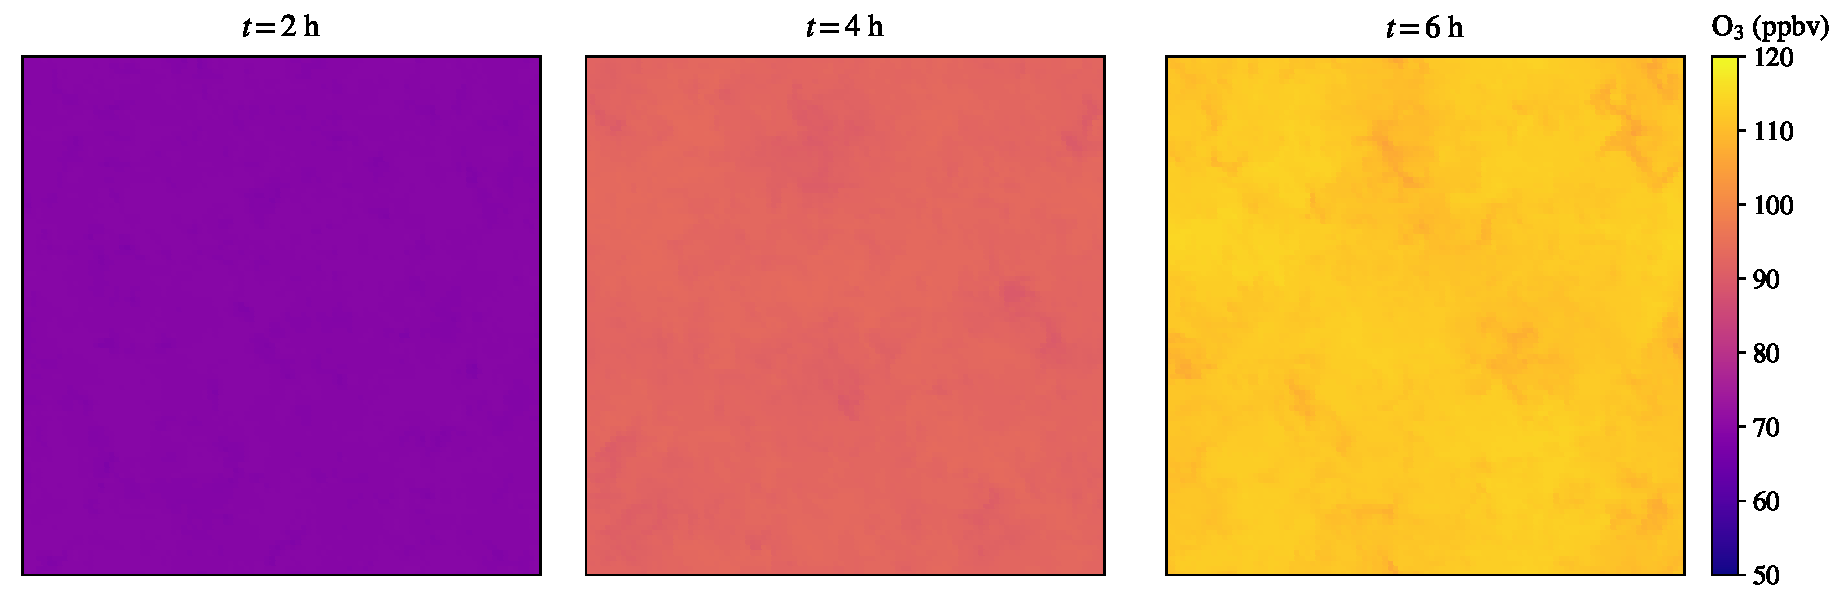
\includegraphics[width=\textwidth]{figures/chapter4/o3-crosssec-uniform-basecase-z25.pdf}
    \caption{Ozone cross sections in the x-y plane at 2 hour intervals in the middle of the PBL ($z\sim500$ \si{m}) for the uniform base case.}
    \label{fig:o3-crosssec-ub}
  \end{figure}

In order to visualize the spatial heterogeneities present in ozone throughout each simulation, cross sections of ozone concentrations in the x-y plane were plotted for each emissions scenario. Cross sections were selected at a vertical level corresponding to the approximate middle of the PBL ($z\sim500$ \si{m}) and were plotted at regular, 2 hour intervals. 

Ozone cross section plots for the uniform base case are shown in Figure \ref{fig:o3-crosssec-ub}. Ozone concentrations are displayed as molar fractions in parts per billion by volume (ppbv). Throughout each snapshot, the distribution of ozone is shown to be nearly uniform with minimal concentration gradients. Ozone concentrations steadily increase throughout the course of the simulation, reaching in excess of 110 ppbv by $t=6$ h.

Ozone cross sections for emission scenarios 1--3 are shown in Figures \ref{fig:o3-crosssec-s1}--\ref{fig:o3-crosssec-s3}, respectively. By $t=2$ h, ozone concentrations have risen from their initial condition of 50 \si{ppbv} to a nearly uniform 60 \si{ppbv} in areas distant from the region where the emissions plume passes through. Approaching the area surrounding the plume, ozone concentrations are lower at  $\sim50$ \si{ppbv}, indicating that very little ozone production occurs in the immediate vicinity of the emissions plume. This trend increases moving from emissions scenario 1 (Figure \ref{fig:o3-crosssec-s1}) to emissions scenario 3 (Figure \ref{fig:o3-crosssec-s3}), where the absence of elevated ozone levels in the central region of the plume is clearly visible. 

\begin{figure}[h]
    \centering
    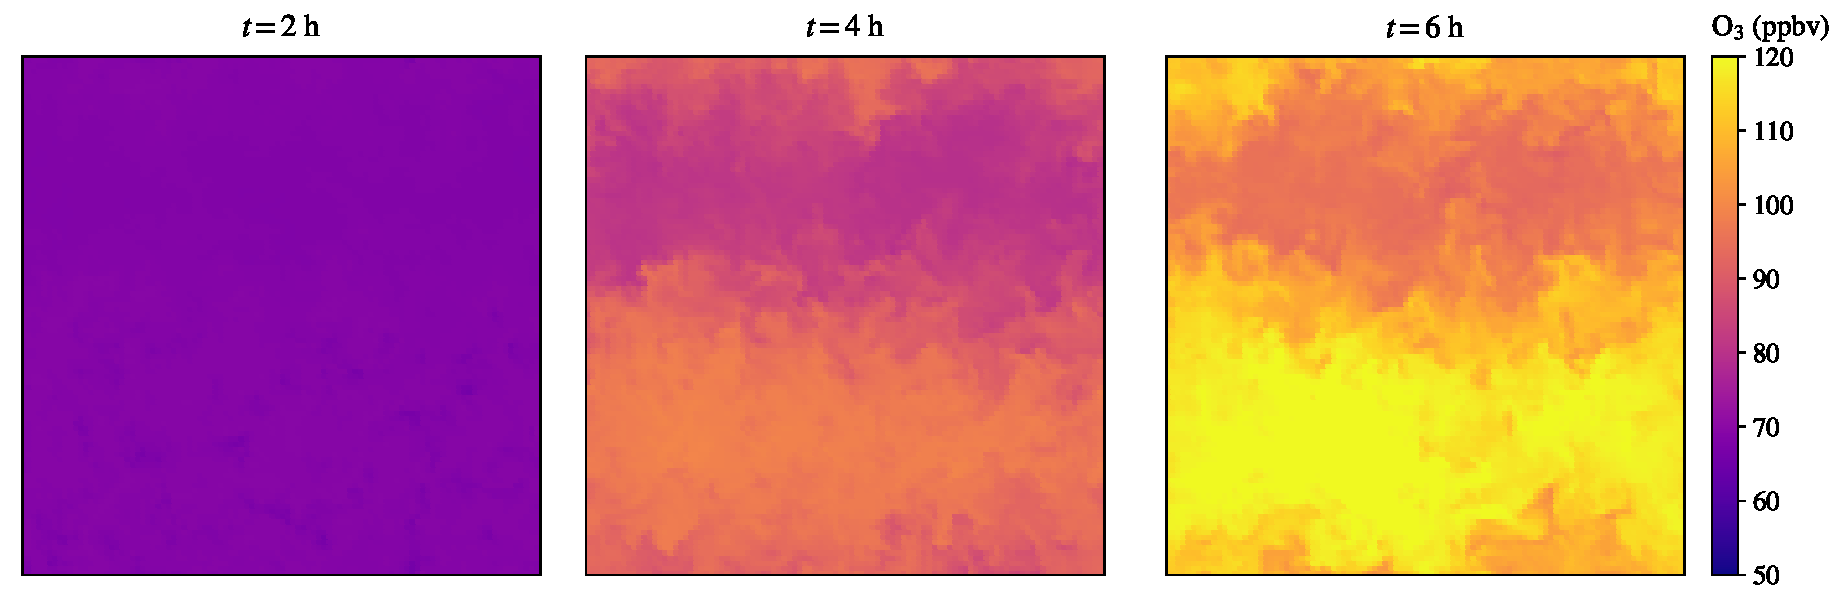
\includegraphics[width=.9\textwidth]{figures/chapter4/o3-crosssec-fx1fy0-z25.pdf}
    \caption{Ozone cross sections in the x-y plane at 2 hour intervals in the middle of the PBL ($z\sim500$ \si{m}) for emissions scenario 1.}
    \label{fig:o3-crosssec-s1}
\end{figure}

\begin{figure}[h]
    \centering
    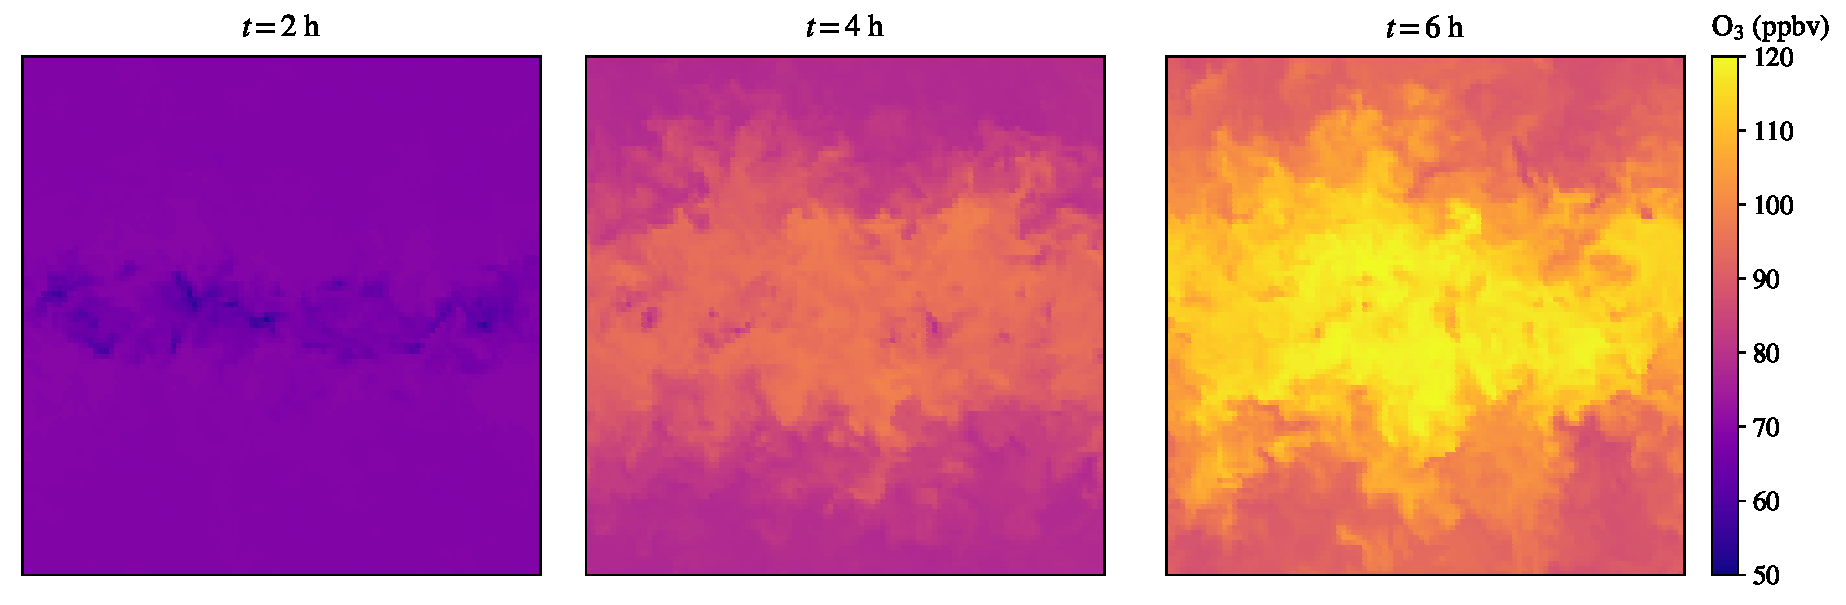
\includegraphics[width=.9\textwidth]{figures/chapter4/o3-crosssec-road-10x-z25.pdf}
    \caption{Ozone cross sections in the x-y plane at 2 hour intervals in the middle of the PBL ($z\sim500$ \si{m}) for emissions scenario 2.}
    \label{fig:o3-crosssec-s2}
\end{figure}

  \begin{figure}[!h]
    \centering
    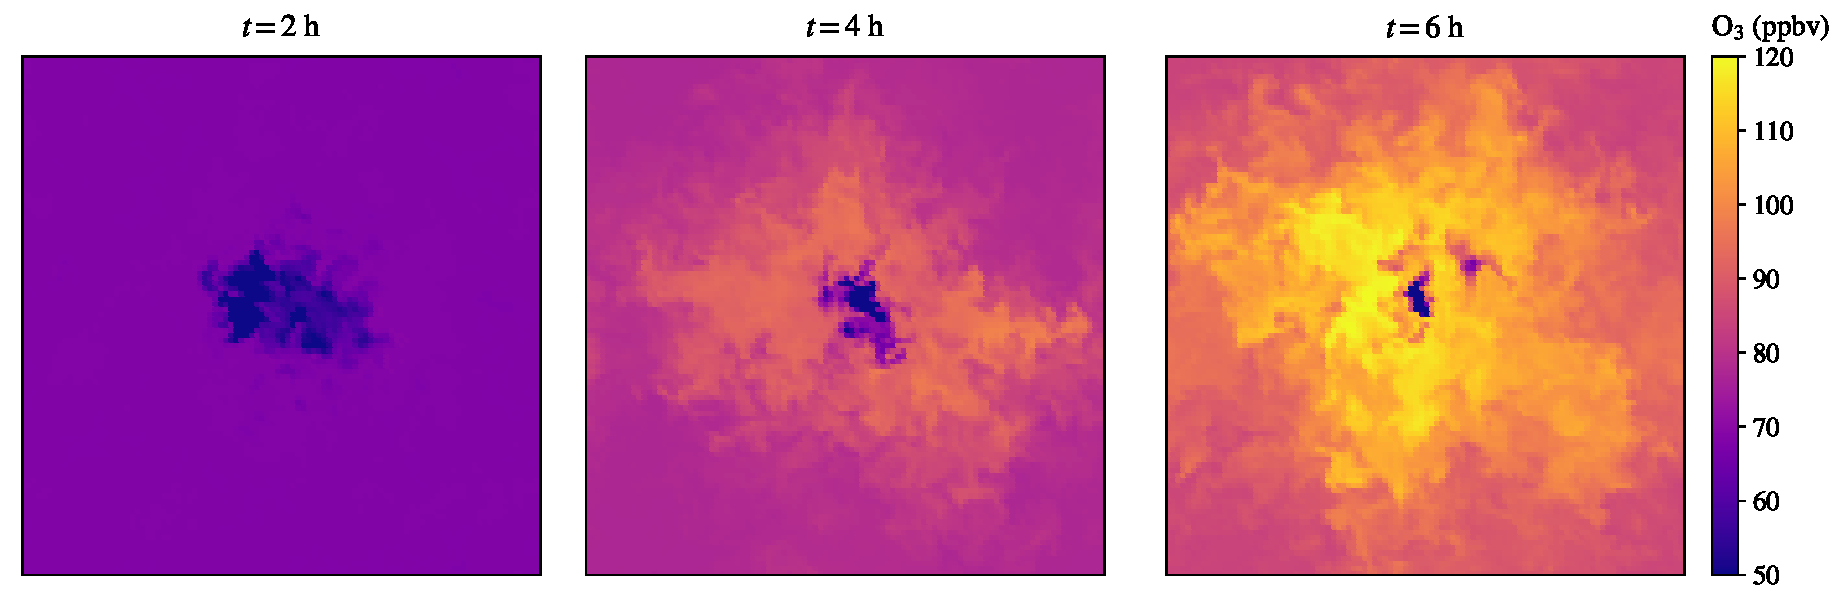
\includegraphics[width=.9\textwidth]{figures/chapter4/o3-crosssec-point-source-1x1-z25.pdf}
    \caption{Ozone cross sections in the x-y plane at 2 hour intervals in the middle of the PBL ($z\sim500$ \si{m}) for emissions scenario 3.}
    \label{fig:o3-crosssec-s3}
\end{figure}

By $t=4$ h and $t=6$ h, ozone concentrations have risen in the region immediately surrounding the plume, reaching upwards of 110 \si{ppbv} in each scenario by $t=6$ h. The region of most efficient ozone production clearly overlaps with the region where the plume is rising through the PBL; however, for the highest spatial heterogeneity emissions scenario, scenario 3 (Figure \ref{fig:o3-crosssec-s3}), we find that ozone concentrations are significantly depressed in the immediate vicinity of the plume. This points to the non-linear nature of ozone production and its dependance on the relative abundance of NO$_x$ and VOCs.

%\subsection{Segregation intensity}
\subsection{Spatio-temporal trends in ozone and its precursors}

\begin{figure}[h]
    \centering
    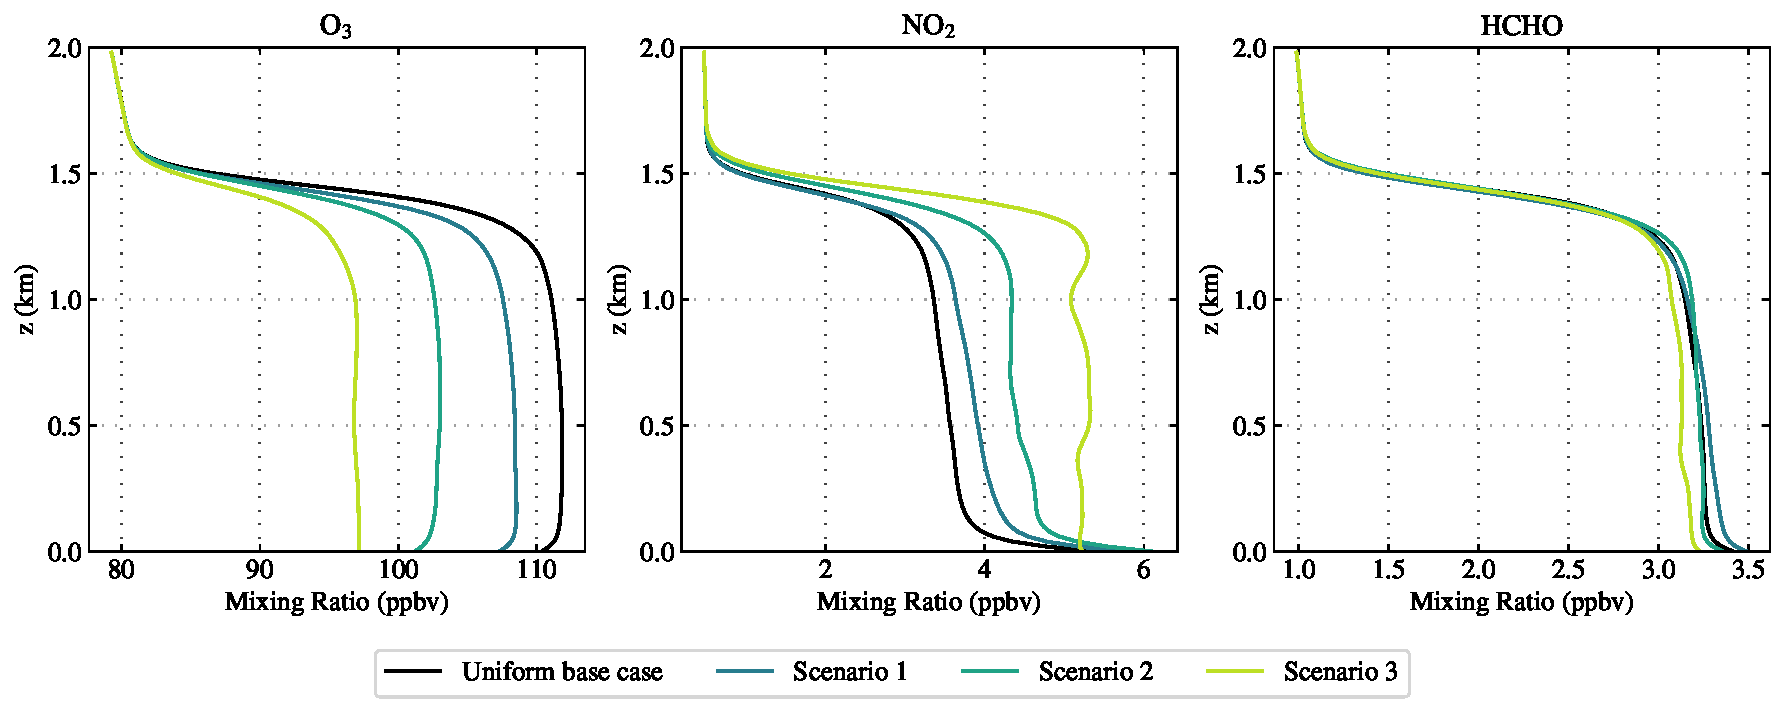
\includegraphics[width=\textwidth]{figures/chapter4/vertical-profiles-time36.pdf}
    \caption{Vertical profiles at $t=6$ h for ozone, NO$_2$, and HCHO (left to right) for each emissions scenario. Each vertical profile indicates the species mean concentration when horizontally averaged at each vertical level.}
    \label{fig:vertical-profiles-o3-nox-hcho}
  \end{figure}
  
Vertical profiles at $t=6$ h for ozone, NO$_2$, and HCHO (formaldehyde) across each emissions scenario are shown in Figure \ref{fig:vertical-profiles-o3-nox-hcho}. For each plot, the vertical profile was computed by determining the horizontal average across the domain of each compound and for each vertical level. NO$_2$ is displayed alongside ozone to evaluate whether NO$_x$ titration is occuring--at high NO concentrations, there is a net conversion of ozone to NO$_2$ via 
\begin{equation}
\ce{O_3 + NO -> NO_2 + O_2}.
\label{eq:nox-titration}
\end{equation}
Usually this reaction is balanced by photolysis of NO$_2$, however, in emissions plumes with high concentrations of NO, Reaction \ref{eq:nox-titration} results in a net conversion of ozone to NO$_2$. HCHO is chosen as a representative VOC.

We find that mean ozone concentrations are nearly uniform in the PBL for each emissions scenario, with a reduction in mean concentrations from $\sim 112$ ppbv in the uniform base case to $\sim 97$ ppbv for emissions scenario 3. By $t=6$ h, the boundary layer height has grown to nearly $z=1.5$ \si{km}, above which point ozone concentrations are nearly identical at $\sim80$ \si{ppbv} across emissions scenarios. Note the initial condition for ozone is a uniform 50 \si{ppbv} throughout the entire domain, indicating that in the absence of additional NO$_x$ and VOC precursors due to emissions, ozone concentrations rise by approximately 30 \si{ppbv} over 6 hours due to ambient precursor concentrations and photolysis reactions.

NO$_2$ concentrations vary considerably within the boundary layer, with concentrations approaching 6 ppbv near the surface followed by a slightly decreasing trend in the middle to upper PBL. We find higher NO$_2$ concentrations as we move from the uniform base case to higher emissions spatial heterogeneity scenarios. We also find that under the highest emissions $SH$ scenarios (scenario 2 and 3), the profile of NO$_2$ is more variable with height.

HCHO concentrations are relatively uniform across each emissions heterogeneity scenario, with concentrations between 3--3.5 \si{ppbv} in the PBL. Agreement in the abundance of HCHO across emission scenarios suggest that it is not as sensitive to emissions spatial heterogeneity as NO$_x$. 
%\hl{probably owing to the rate at which it reacts with other species}.

\begin{figure}[t]
  \centering
    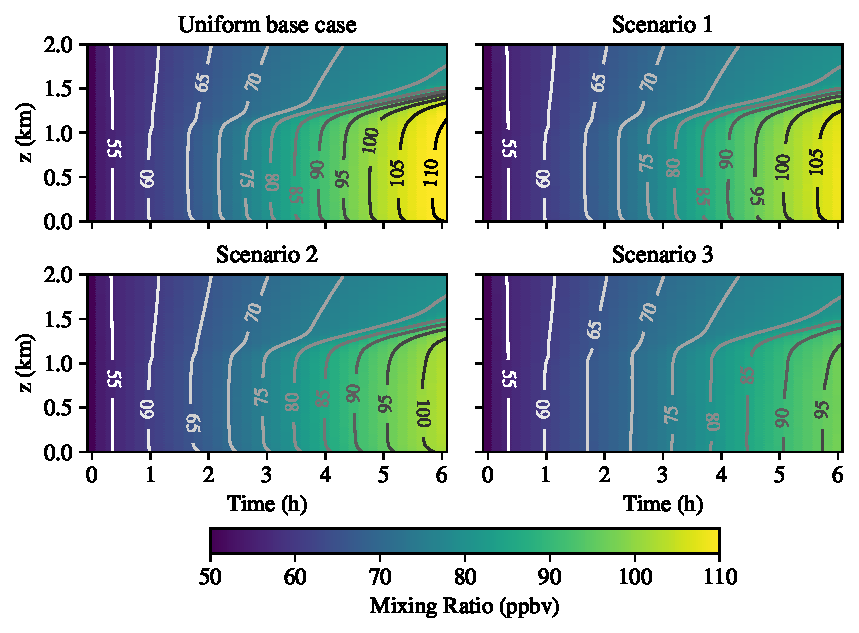
\includegraphics[width=\textwidth]{figures/chapter4/height-time-o3-four-scenarios.pdf}
    \caption{Ozone concentration time-height plots for each emissions scenario.}
    \label{fig:ht-o3}
\end{figure}

Time-height sections of ozone concentrations are shown for each emissions scenario in Figure \ref{fig:ht-o3}. For each time-height figure, the horizontal average concentration of ozone was computed for each vertical level and at time in the simulation output. Isopleths are superimposed on each time-height plot and indicate regions of constant ozone concentrations in increments of 5 ppbv. 

During the first hour of each simulation, ozone concentrations gradually increase nearly uniformly from the initial concentration of 50 ppbv to 60 ppbv. Emissions are turned on at $t=1$ h, however ozone concentrations for emissions scenarios 1--3 do not appear to appreciably diverge from the uniform base case until $t\simeq2$ h and beyond. After this point, ozone concentrations increase in the PBL of each scenario (the PBL height gradually grows throughout the simulation as indicated by the region of highest ozone concentrations due to the constant heat flux at the surface). Ozone concentrations alongside the ozone formation rate are highest in the uniform base case. Note that between hours 5 and 6, ozone concentrations in the PBL increase by approximately 10 ppbv as indicated by isopleths. By comparison, ozone concentrations increase by approximately 5 ppbv for scenario 3 during the same time period.

To quantify the relative difference between ozone production in the uniform base case and each emission scenario, Figure \ref{fig:ht-pdiff-o3} displays time-height plots for each emissions scenario where the percent difference between ozone in the uniform base case and each scenario is displayed with superimposed isopleths. Percent difference is calculated as 
\begin{equation}
    \% \text{ difference} = 100\times\left(\frac{\overline{[O_3]}(t, z)_{\text{Scenario}} - \overline{[O_3]}(t, z)_{\text{Base case}}}{\overline{[O_3]}(t, z)_{\text{Base case}}}\right),
\end{equation}
where $\overline{[O_3]}(t, z)_{\text{Scenario}}$ is the horizontally averaged concentration of ozone at time $t$ and vertical level $z$ for a particular scenario and $\overline{[O_3]}(t, z)_{\text{Base case}}$ is the horizontally averaged concentration of ozone at time $t$ and vertical level $z$ for the uniform base case.

\begin{figure}[h]
  \centering
    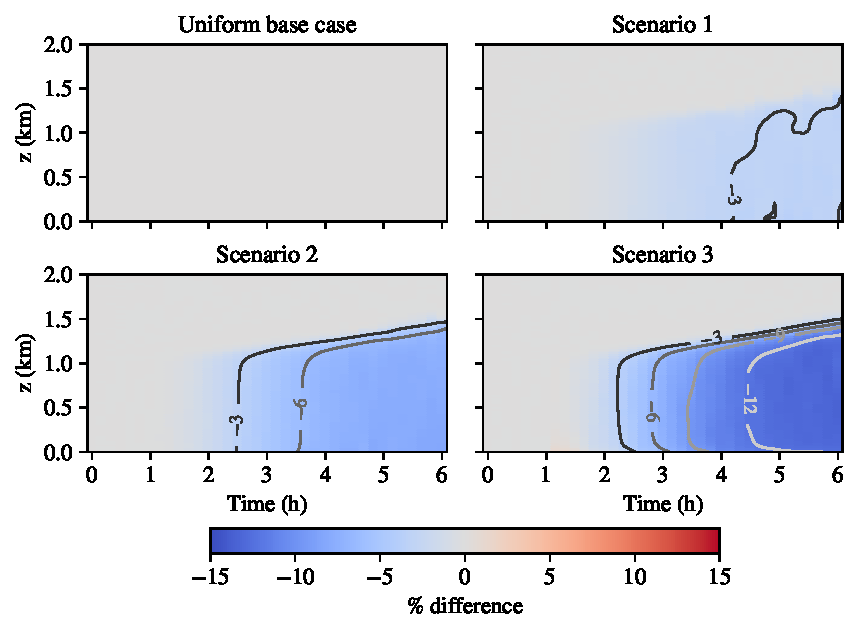
\includegraphics[width=\textwidth]{figures/chapter4/height-time-o3-pdiff-four-scenarios.pdf}
    \caption{Time-height plots of ozone percent difference for each emissions scenario.}
    \label{fig:ht-pdiff-o3}
\end{figure}

In Figure \ref{fig:ht-pdiff-o3} , regions shaded in blue indicate negative percent difference (i.e., the uniform base case contains higher concentrations in a given region) while red indicates positive percent difference. Regions shaded in gray indicate zero percent difference. We find that ozone concentrations for emissions scenario 1 are in good agreement with the uniform base case within the free troposphere during the entire simulation and also in the PBL prior to $\sim$2 hours. After this point, ozone concentrations are up to 3\% less in the PBL through $t=6$ h.

We find similar but heightened trends for ozone concentration percent difference for emissions scenarios 2 and 3, respectively. For scenario 2, ozone concentrations are up to 8\% less in the PBL through $t=6$ h and are reduced by up to $\sim13$\% for scenario 3.

\subsection{Spatial heterogeneity in the atmosphere of ozone and its precursors}

In addition to the spatial heterogeneity of each emission pattern as shown in Figure \ref{fig:ozone-emission-patterns}, once gas phase species are emitted from the surface, their atmospheric distribution will be influenced by the emissions pattern heterogeneity, the strength of mixing, and chemical reactions that alter the abundance of compounds. We refer to the spatial heterogeneity of a gas phase species in the atmosphere as the species' {\it field} spatial heterogeneity. 

\begin{figure}[h]
    \centering
    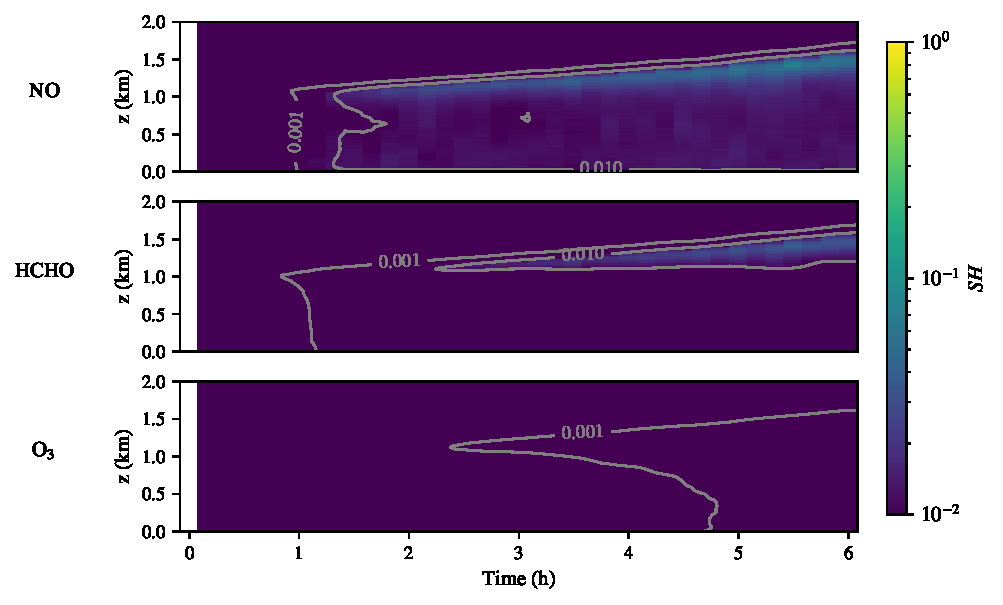
\includegraphics[width=.97\textwidth]{figures/chapter4/height-time-nsh-multivar-uniform-basecase.pdf}
    \caption{Time-height plot of field $SH$ for O$_3$, NO$_x$, and HCHO in the uniform base case. $SH$ value contours are shown in grayscale for each subplot.}
    \label{fig:atmos-sh-ub}
  \end{figure}

Figure \ref{fig:atmos-sh-ub} shows time-height plots of the field spatial heterogeneity for NO (top), HCHO (middle), and ozone (bottom) for the uniform base case. Field $SH$ is computed for horizontal cross sections of the domain at each vertical level and each time. Regions filled with dark blue correspond to low field $SH$ while regions in green and yellow indicate high field $SH$. In Figure \ref{fig:atmos-sh-ub}, the field $SH$ of each compound is very low. After $t=1$ h, NO field $SH$ is $\sim0.01$ within the PBL. HCHO field $SH$ is $\sim0.001$ within the PBL following the release of emissions at $t=1$ h, with slightly higher values of 0.01 near the upper PBL developing after $t=2$ h. Ozone field $SH$ is the lowest of the three compounds, with values of 0.001 developing in the upper PBL after $t=2$ h and extending to the surface by $t=5$ h.

Similarly, Figure \ref{fig:atmos-sh-s1} shows time-height plots for ozone and its precursors for emissions scenario 1. Recall that the emissions $SH$ for scenario 1 is 0.33. Field $SH$ for all species is lower than the emissions $SH$ (as we expect due to atmospheric processes that disperse, dilute, and alter the concentration of each compound). As emissions begin at $t=1$ h, the field $SH$ of NO is $\sim0.1$ within the PBL and increases to 0.2 after approximately 2 hours. Around $t=5$ h, the field SH of NO decreases back down to 0.1 within the PBL. Following the release of emissions at $t=1$ h, HCHO field $SH$ is 0.05, increasing to 0.1 by approximately 2 hours and 30 minutes where it remains for the duration of the simulation. Similar to field $SH$ for the uniform base case, ozone exhibits the lowest field $SH$ of all three species, with values of 0.001 from $t=1$ h to $t=3$, afterward increasing to 0.01.

\begin{figure}[h]
    \centering
    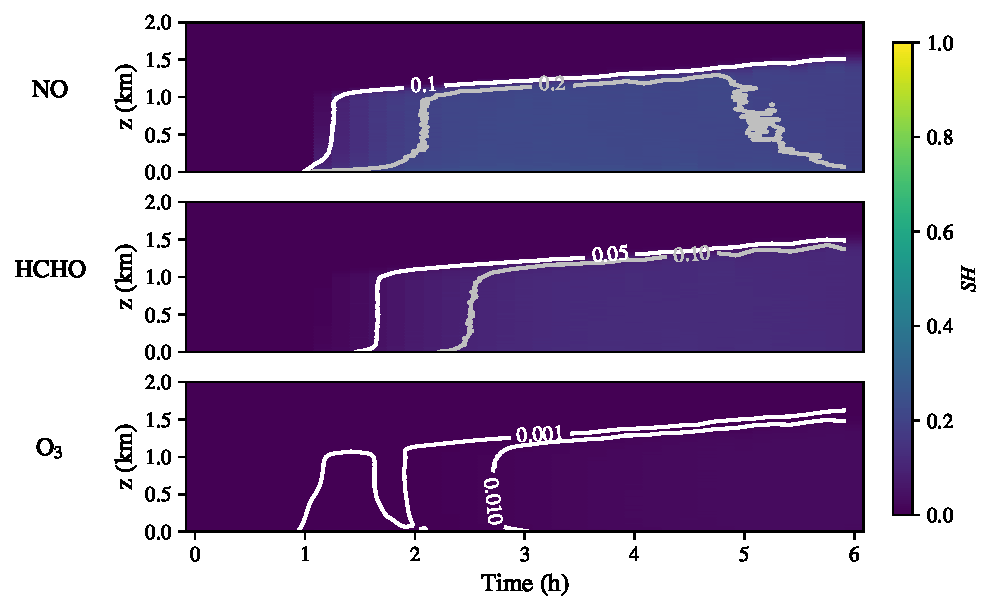
\includegraphics[width=.97\textwidth]{figures/chapter4/height-time-nsh-multivar-fx1fy0.pdf}
    \caption{Time-height plot of field $SH$ for O$_3$, NO$_x$, and HCHO in emissions scenario 1. $SH$ value contours are shown in grayscale for each subplot.}
    \label{fig:atmos-sh-s1}
 \end{figure}
 
We find similar trends to scenario 1 in the field $SH$ of ozone and its precursors for emissions scenario 2 as shown in Figure \ref{fig:atmos-sh-s2}. Recalling that the emissions $SH$ of scenario 2 is 0.60, we find that the field $SH$ of NO and HCHO correspondingly increase compared to scenario 1. Following emissions at $t=1$ h, the field $SH$ of NO in the PBL increases to 0.3 over nearly the entire height PBL except for near the surface where the field $SH$ reaches 0.4. The field $SH$ of HCHO increases to 0.15 by $t=3$ h, where it remains through the duration of the simulation. The pattern of field $SH$ for ozone closely matches its behavior noted for scenario 1--from $t=1$ h to $t=3$ h, ozone field $SH$ is of order 0.001, increasing to 0.01 afterwards.

\begin{figure}[h]
    \centering
    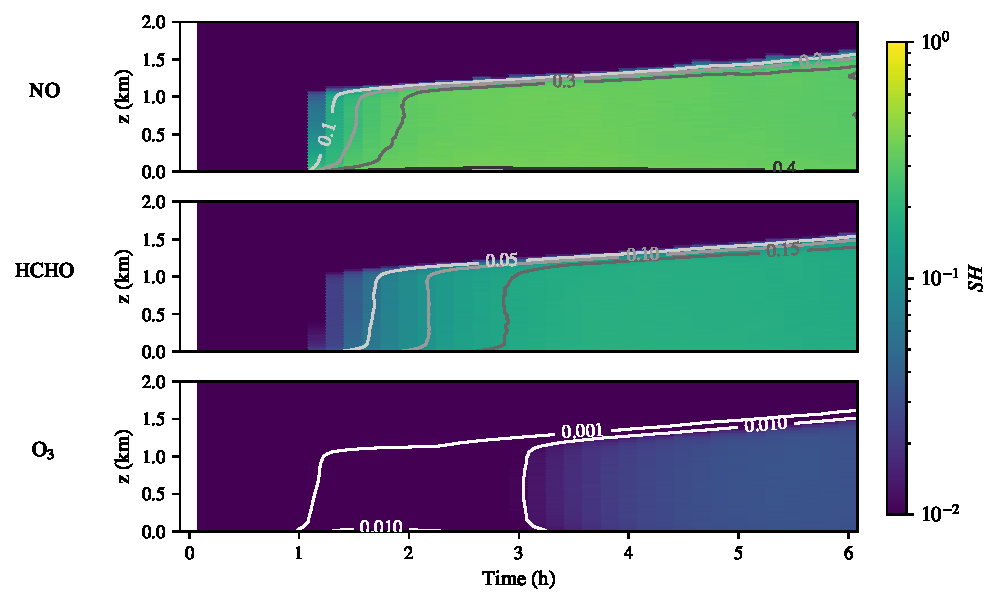
\includegraphics[width=.97\textwidth]{figures/chapter4/height-time-nsh-multivar-road-10x.pdf}
    \caption{Time-height plot of field $SH$ for O$_3$, NO$_x$, and HCHO in emissions scenario 2. $SH$ value contours are shown in grayscale for each subplot.}
    \label{fig:atmos-sh-s2}
\end{figure}

  \begin{figure}
    \centering
    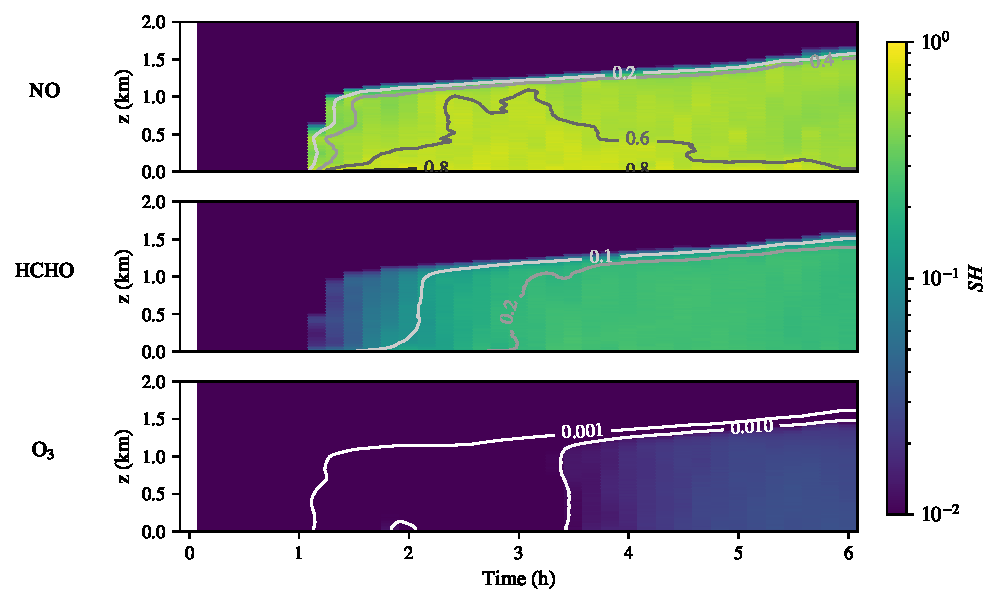
\includegraphics[width=.97\textwidth]{figures/chapter4/height-time-nsh-multivar-point-source-1x1.pdf}
    \caption{Time-height plot of field $SH$ for O$_3$, NO$_x$, and HCHO in emissions scenario 3. $SH$ value contours are shown in grayscale for each subplot.}
    \label{fig:atmos-sh-s3}
 \end{figure}
 
Figure \ref{fig:atmos-sh-s3} shows the field $SH$ of ozone and its precursors for emissions scenario 3. Scenario 3 posses the highest emissions spatial heterogeneity, $SH=1$. As a result, the field $SH$ of both NO and HCHO are markedly higher compared to previous scenarios. Field $SH$ of NO varies both spatially and temporally for scenario 3. Following the release of emissions at $t=1$ h, we find a high field $SH$ of 0.8 near the surface that persists for the duration of the simulation. Moving up in the PBL, field $SH$ ranges from 0.4 to 0.6. From $t=1$ h to $t=2$ h, the region of high field $SH$ at 0.6 is localized near the surface. Following this point, this high field $SH$ region extends upwards to the top of the PBL from  $t=2$ h to $t=3$ h. After this point, field $SH$ lowers back down to 0.4 over most of the PBL. Field $SH$ of HCHO is relatively uniform through the PBL and increases following emissions to 0.2 by $t=3$ h where it remains for the duration of the simulation. Similar to the field $SH$ of ozone discussed for scenarios 1 and 2, ozone exhibits a very similar pattern for scenario 3--from $t=1$ h to $t=3.5$ h, ozone field $SH$ is of order 0.001, increasing to 0.01 afterwards.

%\hl{Decrease in NO field sh seems to occur around the same time that HCHO field sh increases, shortly followed by ozone. My theory is that this may point to changes in ozone production efficiency as the relative abundance of NOx changes due to continued emissions and perhaps the VOCs are reacting more to produce more ozone (thus increasing the conc. and coupling the field sh of ozone to VOC field sh?) Its also the case that there ARE aerosols in these simulations and that presents an important pathway for the removal of NOx via nitric acid to form aerosol nitrate and nitric acid deposition.}


%\subsection{Structural uncertainty in ozone production}

%\begin{figure}[h]
%    \centering
%    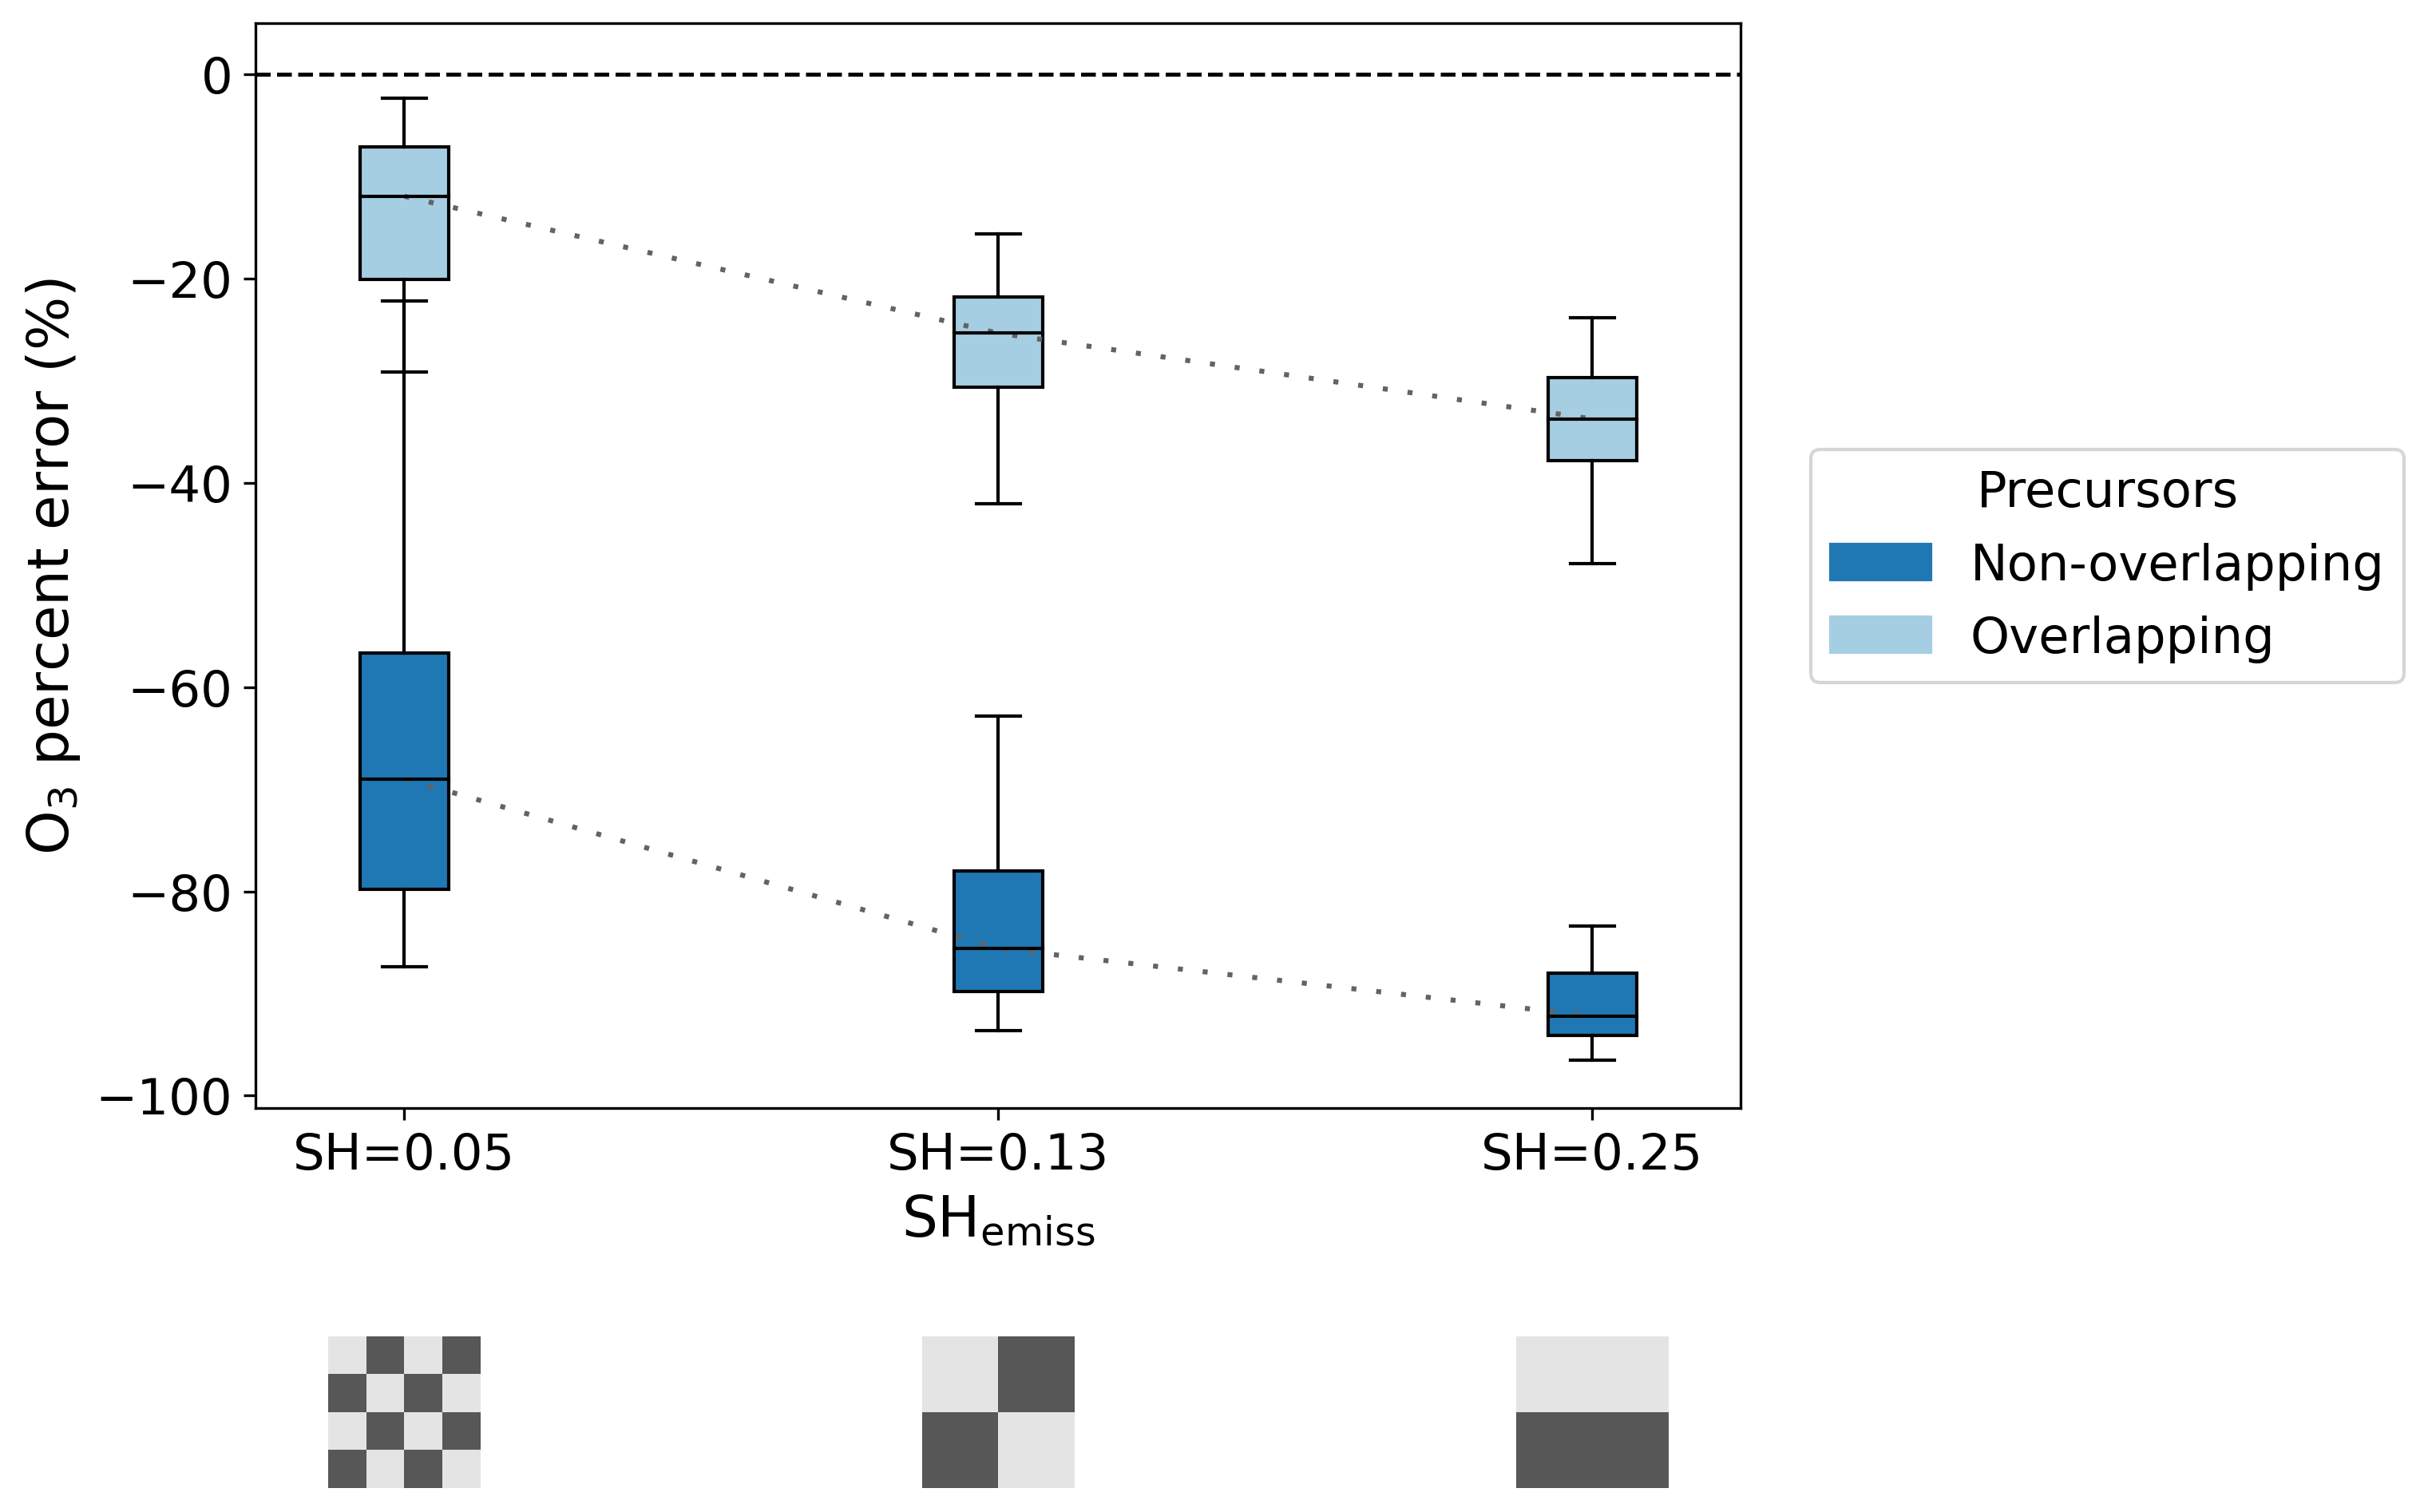
\includegraphics[width=\textwidth]{figures/O3-percent-err-vs-emiss-SH.png}
%    \caption{\hl{Via ARM poster:} Deviation of ozone concentration from case with uniform NOx and VOC emissions. Larger SH in emissions and overlapping emissions lead to larger deviations.}
    %\label{fig:aero_ic_dist}
%  \end{figure}
  
\section{Discussion}

We find an inverse relationship between emissions spatial heterogeneity and the production of ozone; as emissions become more spatially heterogeneous, ozone concentrations are reduced by up to 12\% within the PBL. Additionally, increases in the field $SH$ of ozone precursors are observed under high emissions $SH$ scenarios with the highest magnitude of field $SH$ observed for NO. By comparison, the field $SH$ of ozone is low (field $SH<0.01$) across all emissions scenarios. 

% Perhaps the field SH of ozone is low because it is reacting very quickly, i.e., whatever gets produced is subsequently removed, thus reducing any concentration gradients or local hotspots that may otherwise increase field SH. This kind of contradicts my hypothesis that the NOx titration mechanism is responsible for ozone removal though, since NO has pretty high field SH in the highest heterogeneity scenario. One could alternatively argue that the reaction rate of NO is very high which is why it has the highest field SH (the region of NO remains concentrated since its reacted away and doesnt get the chance to be diffused out to the point of having lower SH). Another thing is that ozone is not emitted, but rather produced everywhere in the domain. This rate varies depending on where you are relative to the plume, but on net this should lead to more diffuse distribution of ozone.

The production of ozone in the PBL has been thoroughly studied, including the use of LES to investigate the impacts of chemically segregated emissions and turbulence-chemistry interactions. \cite{schumann_large-eddy_1989} conducted an idealized LES study of the PBL to determine the impacts of varying turbulent diffusion strength on generic binary reactions. For rates typical of the ozone-NO$_x$ mechanism, the authors found that reaction rates are significantly impacted by turbulence and chemical segregation. Subsequently, \cite{sykes_large-eddy_1992} conducted a similar LES study of the PBL, however they directly modeled the ozone removal mechanism via NO shown in Reaction \ref{eq:nox-titration}. They showed that the removal of ozone by Reaction \ref{eq:nox-titration} is highly dependent on the strength of turbulent mixing of an emissions plume. Under strong mixing, the plume is more rapidly diffused, reducing the rate of ozone removal and allowing ozone production mechanisms to proceed. Our findings point to a similar conclusion, whereby highly concentrated and spatially heterogeneous emissions of ozone precursors lead to efficient removal of ozone within the plume, resulting in the production of greater NO$_2$. 

Enhancements in removal mechanisms are observed at high emissions spatial heterogeneity. We find that the opposite is true for ozone production. Note that ozone production occurs on short timescales and that low spatial heterogeneity emissions scenarios with more uniform and dilute distributions of precursors result in a longer duration of time in which precursors remain well mixed. This effectively enhances the timescale over which ozone production can occur, leading to higher ozone concentrations. Recall that the uniform base case emissions scenario serves as a proxy for coarser resolved models in which emissions spatial heterogeneity on length scales smaller than the grid resolution will not be resolved. Thus, we may expect model comparisons of ozone production at coarser resolution to over-predict tropospheric ozone concentrations. Indeed, \cite{wild_global_2006} evaluate the production of ozone in a global chemistry model across various grid resolutions and find that ozone production is overestimated near emissions sources by up to 27\% for the coarsest resolution evaluated ($5.6^{\circ}$ x $5.6^{\circ}$) and error scales approximately monotonically as resolution increases. 


%\begin{itemize}
%\item \cite{krol_effects_2000} Maybe?
%\item \cite{auger_chemical_2007} (seems very similar to what I am doing here) LES of PBL over 10x10 km domain. Indicate that segregation is strongest in the first two hours - after 3 hours segregation is largely reduced due to efficient mixing in the PBL. 
%\item \cite{zhong_modelling_2015} Similar to Zhong et al 2017, find that ozone production rate is reduced due to incomplete mixing.
%\item \cite{zhong_large_2017} LES study of O3-NOx-VOC chemistry in urban street canyons characterized by high spatial variability in concentration gradients. NOx and HOx radicals were consumed to produce NO2 and O3. Segregation effect due to incomplete mixing reduces the production of NO2. 
%\item \cite{wang_impact_2021}
%\item \cite{wang_segregation_2022} Similar to wang 2023
%\item \cite{wang_coupled_2023} Use of LES (WRF-Chem LES \hl{what chem mechanism?}) for urban (Hong Kong) emissions compared against mesoscale simulations, show that NOx is underestimated and O3 overestimated in mesoscale simulations when compared to LES, attributed to the higher spatial resolution of emissions and explicitly resolving turbulent transport.
%\end{itemize} 





% !TEX root = ./main.tex
\chapter{Impacts of emissions spatial heterogeneity on aerosol properties and CCN activity}
%\chapter{Impacts of emissions spatial heterogeneity on aerosol properties in a particle resolved framework}

This chapter presents results for the impacts of emissions spatial heterogeneity on aerosol properties, including changes to the aerosol size distribution, composition, mixing state, and CCN activity. We begin with a set of simplified simulations to isolate the effect of spatial heterogeneity on an important aerosol process, coagulation. Subsequently, we present simulation results for full multiphase (gas and aerosol) chemistry runs and discuss changes to aerosol properties and CCN activity. We find that under high emissions spatial heterogeneity, up to 25\% more CCN activate in the upper boundary layer for supersaturations in the range $S=0.3\%$ to $S=0.6\%$. The effects of ammonium on CCN activity are also explored, as we find that high spatial heterogeneity scenarios allow more nitrate in the aerosol phase due to the availability of free ammonia.
\section{Idealized coagulation simulations}

Prior to discussing simulations utilizing the full multiphase chemical mechanism for aerosols and chemistry, we first focus our discussion on the impact of spatial heterogeneity on aerosol number concentration due to coagulation. Coagulation is a primary mechanism for aerosol aging and its rate scales with the square of the number concentration of particles, thus making it an important aerosol process for which to evaluate the impacts of spatial heterogeneity. 

\subsection{Simulation scenarios}

\begin{figure}[h]
  \centering
    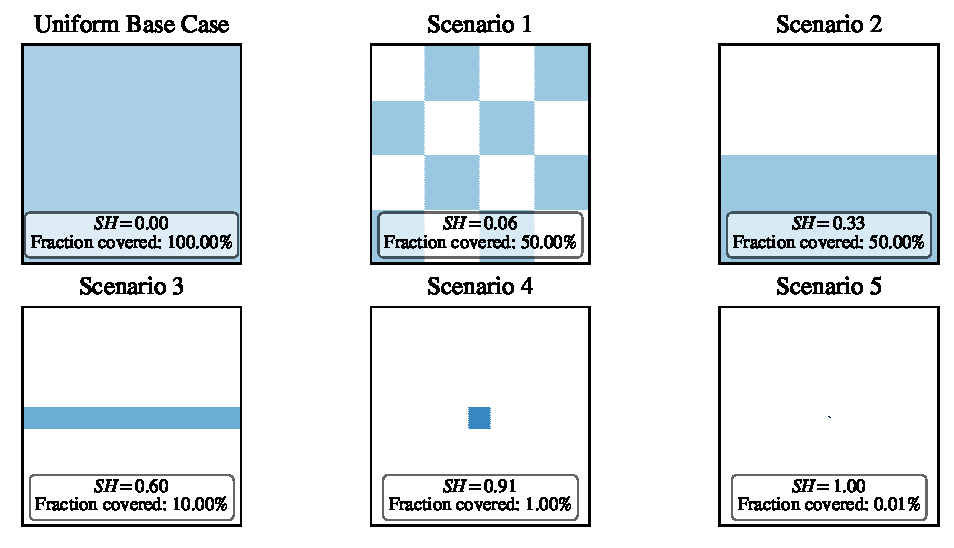
\includegraphics[width=\textwidth]{figures/chapter5/ideal-coag/ideal-coag-SH-scenarios.pdf}
    \caption{$SH$ scenarios for ideal coagulation simulations. The color of each scenario indicates the scaling required to ensure total mass of gas species and aerosols is the same across each scenario, with darker hues indicating a higher degree of scaling.}
    \label{fig:sh-scenarios-ideal-coag}
\end{figure}

Here we investigate the modification to the rate of coagulation under numerous spatial heterogeneity scenarios. We run a total of 6 simulations for a range of $SH$ scenarios shown in Figure \ref{fig:sh-scenarios-ideal-coag}. As with gas phase simulations in Chapter 4, the concentration of atmospheric constituents (here aerosol particle number concentration) must be scaled within the $SH$ scenario region by the ratio of the area of the uniform base case and the area occupied by the $SH$ pattern. For example, the aerosol number concentration in the central region of scenario~5 is a factor of 10,000 higher than in the uniform base case. 

Note that the setup of these simulations differs from all other simulations discussed in this thesis. Chemistry is turned off primarily for computational efficiency as, here, we are simply interested in changes to the number concentration rather than changes to aerosol composition. Instead of using initial conditions that are uniform throughout the domain, here the aerosol initial condition is set by the chosen $SH$ scenario for each vertical level in the domain (i.e., the pattern extends vertically throughout the domain). Additionally, emissions are turned off such that only coagulation is responsible for changes to aerosol number concentration.

\subsection{Results}\label{ideal-coag-results}

\begin{figure}[!h]
  \centering
    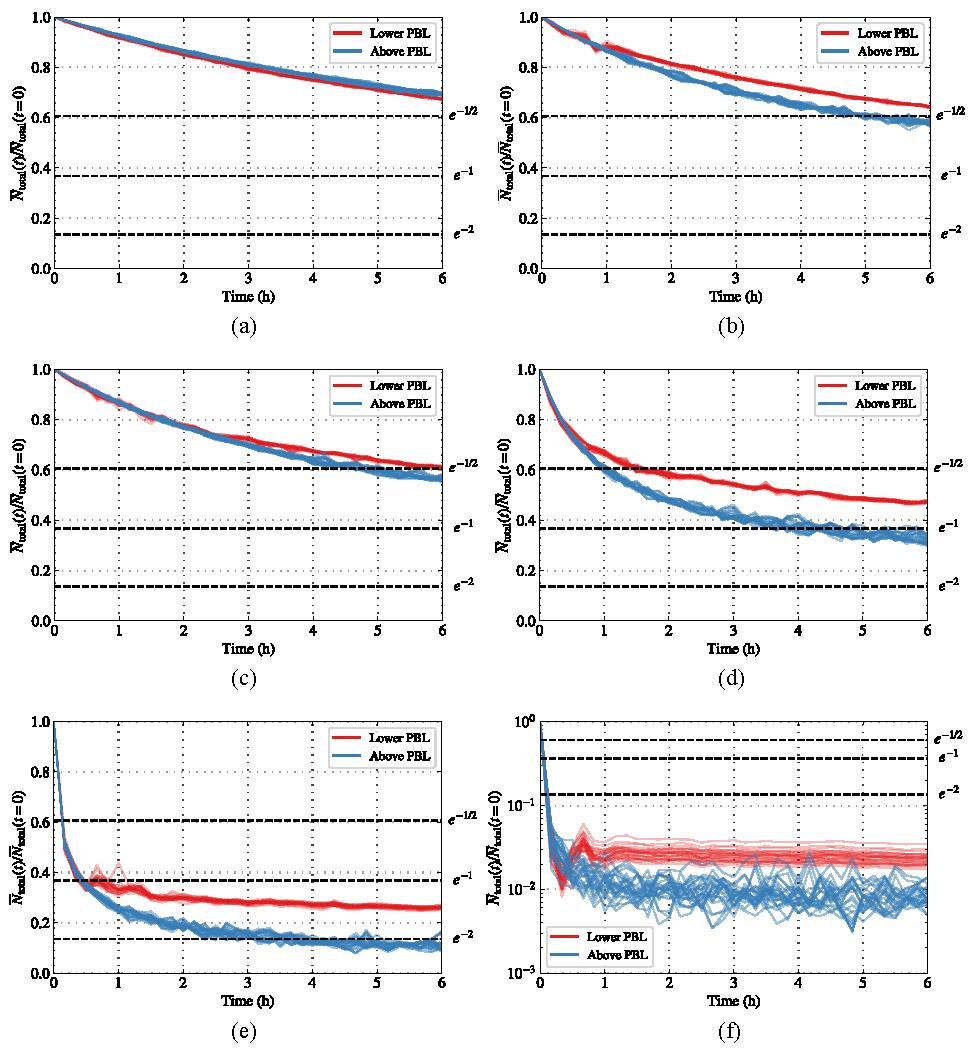
\includegraphics[width=\textwidth]{figures/chapter5/ideal-coag/NumConcTimescale_composite.pdf}
    \caption{Total number concentration for each $SH$ scenario normalized by the initial condition total number concentration. Lines indicate normalized number concentration averaged over each vertical level in the domain. (a) Uniform base case. (b--f) Scenarios 1--5}
    \label{fig:numconc-timescales}
\end{figure}

Figure \ref{fig:numconc-timescales} show how the total number concentration of aerosol particles decreases due to coagulation under each $SH$ scenario. For each scenario, we compute the average number concentration at each vertical level and time $t$, $\overline{N}_{\text{total}}(t)$. This number concentration is then normalized by the number concentration at time $t=0$, $\overline{N}_{\text{total}}(t=0)$. A subset of number concentration timeseries are shown in Figure \ref{fig:numconc-timescales} for the lowest 20 vertical levels of the planetary boundary layer ($z=0$ m to $z\approx200$ m) and highest 20 vertical levels in the domain above the planetary boundary layer ($z\approx1.8$~km to $z=2$~km). The reason for this grouping is that these two regions are notably different in terms of the rate at which the total number concentration decreases. For scenarios 1--5 (Figure \ref{fig:numconc-timescales} subfigures b--f), we find that the total number concentration decreases slower in the lower planetary boundary layer than above the planetary boundary layer. A notable exception to this trend is the uniform base case (Figure \ref{fig:numconc-timescales} subfigure a). Recall that the rate of coagulation scales as the square of the number of particles. As a result, highly heterogeneous patterns that require significant scaling up of the number concentration will have greater rates of coagulation within the high-concentration region associated with the $SH$ pattern. As the planetary boundary layer develops and turbulent motion begins to diffuse the initial structure of the $SH$ pattern, concentration gradients are reduced, resulting in a reduction of the rate of coagulation. This turbulent motion does not disturb the structure of the $SH$ pattern above the planetary boundary layer, and thus coagulation will proceed at a faster rate within the high concentration region of the $SH$ pattern.

We find that as the $SH$ increases across scenarios, the total number concentration is reduced more rapidly. For each plot in Figure \ref{fig:numconc-timescales}, we include horizontal dashed lines indicating the e-folding time alongside a half e-folding time ($e^{-1/2}$) and double e-folding time as the rate at which the total number concentration is reduced under $SH$ scenarios varies widely.  

\begin{figure}[!t]
  \centering
    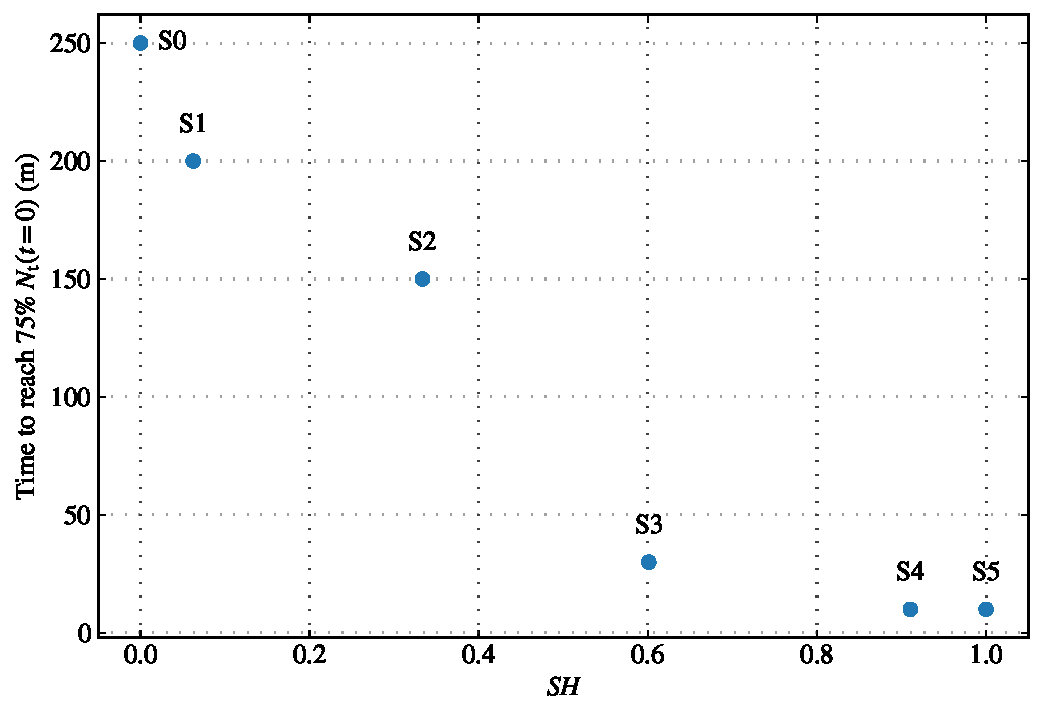
\includegraphics[width=.8\textwidth]{figures/chapter5/ideal-coag/TimeTo75pcnt_vs_SH.pdf}
    \caption{Time required in minutes for the total number concentration in the lowest 200 m of the planetary boundary layer to be reduced to 75\% of the initial value vs. scenario~$SH$. ``S0" is the uniform base case, with all other scenarios labeled S1--S5.}
    \label{fig:numconc-timescales-to-75pcent}
\end{figure}

Figure \ref{fig:numconc-timescales-to-75pcent} shows the time required the number concentration in the lower planetary boundary layer to be reduced to 75\% of the initial total number concentration plotted against the spatial heterogeneity of each scenario. The uniform base case (``S0") requires over four hours to reach 75\% of the initial total concentration, while the highest heterogeneity scenarios 4 and 5 require only 10 minutes. 

These simulations indicate that the number concentration of aerosol particles is highly sensitive to the spatial heterogeneity of the aerosol particle distribution within the domain.  This is due to enhanced coagulation under scenarios with highly spatially heterogeneous and localized patterns characterized by high number concentrations. Coagulation also alters the size distribution of aerosol particles, which we explore further with full multiphase simulations in Section \ref{size-dists}

% --------------------------------------------
\section{Full multiphase simulations}

Here we discuss simulations containing full multiphase chemistry under numerous emissions spatial heterogeneity scenarios. A summary of emissions scenarios is presented followed by presentation of results pertaining to the aerosol state and properties under each emission scenario. 

\subsection{Simulated emissions scenarios}

\begin{figure}[t]
  \centering
    \includegraphics[width=.6\textwidth]{figures/SH-scenarios-main-runs.pdf}
    \caption{Emissions scenarios for multiphase chemistry simulations. The spatial heterogeneity of each emission scenario is listed in the lower portion of each subplot alongside the fraction of the domain covered by emissions patches. The color of each emission region indicates the scaling required to ensure total mass of emitted species per unit time is the same across each scenario, with darker hues indicating a higher degree of scaling.
}
    \label{fig:aerosol-emission-scenarios}
\end{figure}

Scenarios discussed in this section match the set of emissions scenarios presented in Chapter 4 Section \ref{gas-emission-scenarios}. We evaluate changes to the aerosol population under four scenarios with increasing spatial heterogeneity as shown in Figure \ref{fig:aerosol-emission-scenarios}. As with previous results, the first scenario is a ``uniform base case", characterized by diffuse and uniform emissions across the ground level of the domain ($SH=0$). Scenarios 1--3 present progressively higher heterogeneity up to $SH=1$, whereby the rate of emissions is scaled to ensure the total mass per unit time emitted across each scenario is the same.

As a reminder to the reader, initial conditions and emissions for the gas phase and aerosol are discussed in Chapter 3 Section \ref{gas-phase-ics-and-emiss} and Section \ref{aerosol-ics-and-emiss}, respectively. 

\subsection{Aerosol size distributions}\label{size-dists}

\begin{figure}[!t]
  \centering
    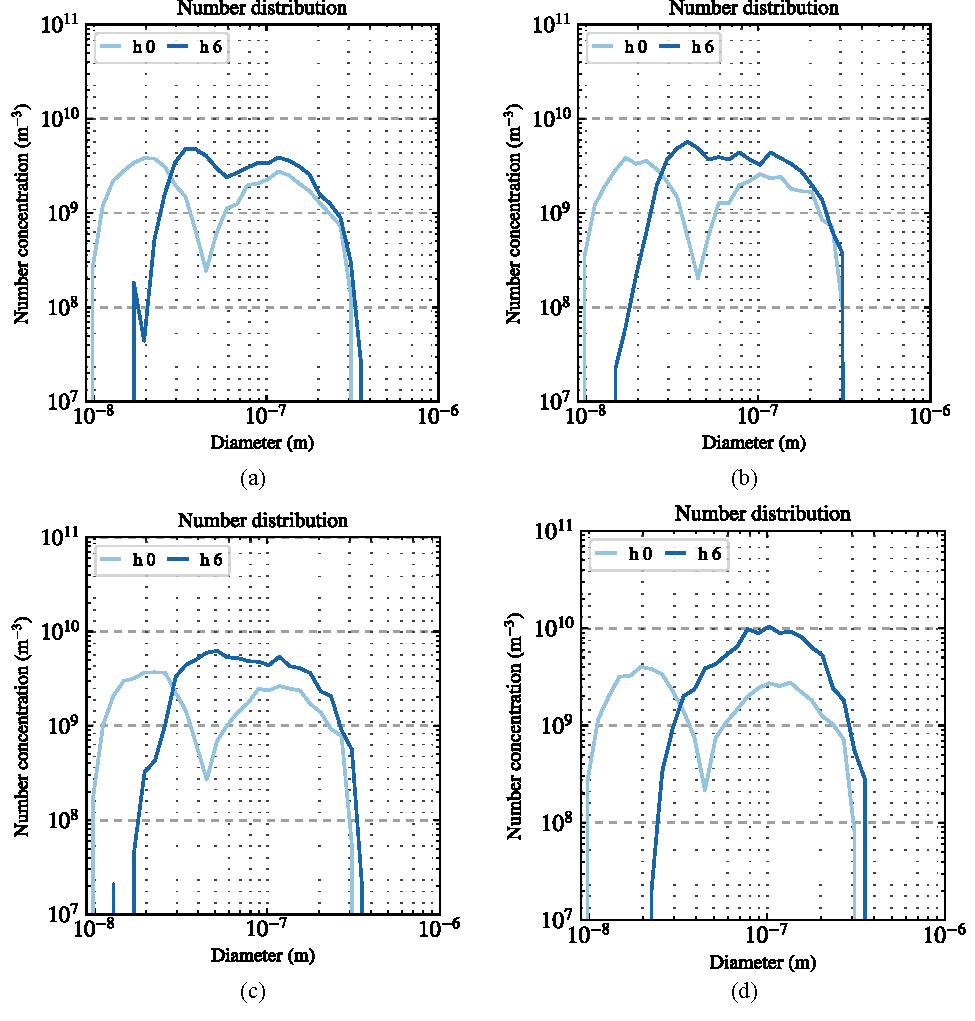
\includegraphics[width=\textwidth]{figures/chapter5/number-distribution-plots.pdf}
    \caption{Aerosol number distribution plots for each emissions scenario. The distribution initial condition (light blue) is shown alongside the distribution at the end of each simulation ($t=6$ h).}
    \label{fig:number-dists}
\end{figure}

Figure \ref{fig:number-dists} shows aerosol number distributions for each simulated emissions scenario. The initial condition size distribution is presented alongside the size distribution at the end of each simulation ($t=6$ h). Each size distribution is taken from a vertical level in the upper boundary layer at $z\approx800$~\si{m}. Due to the stochastic treatment of aerosols in the WRF-PartMC model and the chosen number of computational particles per grid cell ($n=100$), size distributions represent the average distribution in a 1 \si{km^2} region centered over the emissions plume. For all scenarios except scenario~1, this region is located at the center of the domain. For scenario~1, emissions are released in one half of the domain that is offset from the center, thus the averaging region for the size distribution is located in the center of the emissions patch. WRF-PartMC returns the number distribution in 100 logarithmically spaced bins ranging from $10^{-9}$ m to $10^{-3}$ m.

For each scenario displayed in Figure \ref{fig:number-dists}, the initial condition size distribution is shown in light blue. The distribution is bimodal, containing an Aitken (left) and accumulation mode (right). The Aitken mode contains fine particulates and is centered around $20$~nm, while the accumulation mode contains slightly fewer particles and is centered around 116~nm. 

After 6 hours, the number of particles with diameter smaller than $\approx30$~nm is significantly reduced as these small particles undergo coagulation and growth by gas-to-particle partitioning. For particle diameters greater than $\approx30$~nm, the number concentration is increased under each scenario as primary aerosol are emitted and particles undergo aging. For the uniform base case, the distribution still takes on a bimodal shape at $t=6$ h, however the Aitken mode has been replaced by a mode centered around 35~nm and is a combination of primary aerosol and aged aerosol due to gas-particle partitioning and coagulation of Aitken mode particles (see Section \ref{aero-comp} for discussion of size-resolved aerosol composition). 

Moving to higher emissions spatial heterogeneity scenarios, we find that the number distribution loses its bimodal shape after 6 hours, especially under the highest heterogeneity scenario, scenario~3. For scenario~3, the number distribution peaks around 0.1~$\mu$m. Compared with the uniform base case, the number concentration of particles in the accumulation mode near $D_p = 0.1$~\si{\mu m} is approximately half an order of magnitude higher~($10^{10}$~\si{m^{-3}} vs. $4\cdot10^9$~\si{m^{-3}}).

Brownian coagulation, or the collision of particles due to Brownian motion, is the dominant coagulation mechanism for submicron particles and is thus the primary manner by which particles coagulate in simulations discussed in this thesis.  As discussed previously, the rate of coagulation scales with the square of the number of particles. In addition, the Brownian coagulation coefficient $K_{12}$ for the collision of particles $1$ and $2$ with diameters $D_{\text{p}1}$ and $D_{\text{p}2}$, respectively, is highly dependent on the relative size of each particle. $K_{12}$ reaches a maximum where the relative size difference between particles is greatest, such that the coagulation of ultrafine particles with larger diameter particles is favored. As shown in Figure \ref{fig:number-dists}, this effectively results in a removal of particles from the Aitken mode as they collide with larger particles in the accumulation mode. As a result, the size distribution shifts towards larger particles for scenarios with high emissions spatial heterogeneity.

\begin{figure}[!t]
  \centering
    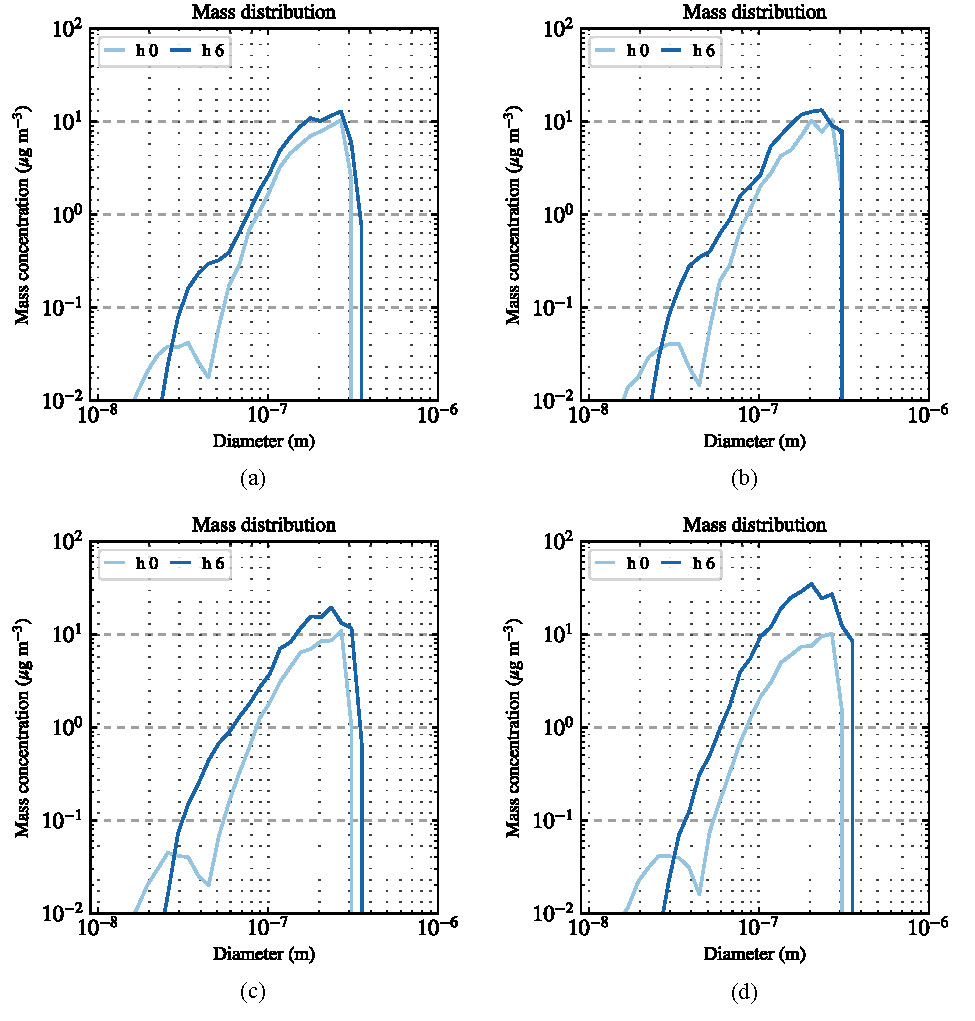
\includegraphics[width=\textwidth]{figures/chapter5/mass-distribution-plots.pdf}
    \caption{Aerosol mass distribution plots for each emissions scenario. The distribution initial condition (light blue) is shown alongside the distribution at the end of each simulation ($t=6$ h).}
    \label{fig:mass-dists}
\end{figure}

Figure \ref{fig:mass-dists} shows mass distribution plots for each emissions scenario. Mass distributions were taken from the same upper boundary layer region as number distributions and the same averaging technique was applied over a 1 \si{km^2} region centered over the emissions plume. Mass concentrations are presented in \si{\mu g.m^{-3}}. 

The mass distribution initial condition presents a bimodal profile as before; however, much more mass is concentrated in the larger accumulation mode particles due to the cubic scaling between mass and particle diameter, $M_p \propto D_p^3$. After six hours, the mass concentration of all particles with diameters larger than $\approx25$~nm is increased. The distribution for the uniform base case contains two distinct modes, one corresponding to the accumulation mode and an additional mode centered around $35$~nm. This matches the diameter range of the fine mode observed in number distributions for the uniform base case, indicating the presence of emitted primary aerosol and aged aerosol due to gas-particle partitioning and coagulation of Aitken mode particles. 

As with the number distributions, when moving from low to high $SH$ scenarios, the bimodal shape of the mass distribution is replaced by a single mode centered around the accumulation mode, peaking at $D_p = 0.2$~\si{\mu m}. When compared to the uniform base case, mass concentrations in the accumulation mode for the highest $SH$ case, scenario~3, are approximately 3 times higher ($\approx30$~\si{\mu g.m^{-3}} vs. $\approx10$~\si{\mu g.m^{-3}}). As discussed previously, the removal of the Aitken mode under high emissions spatial heterogeneity scenarios is due to the coagulation of small particles with larger particles in the accumulation mode. While this does transfer the mass of small particles to the accumulation mode, coagulation alone is not enough to explain the increase in accumulation mode mass concentration. This is in large part due to increased gas-particle partitioning of compounds such as ammonia and nitric acid into the aerosol phase where they form ammonium nitrate. These compositional changes due to emissions spatial heterogeneity are discussed in detail in Section \ref{aero-comp}.


\subsection{Aerosol composition}\label{aero-comp}

\begin{figure}[!t]
  \centering
    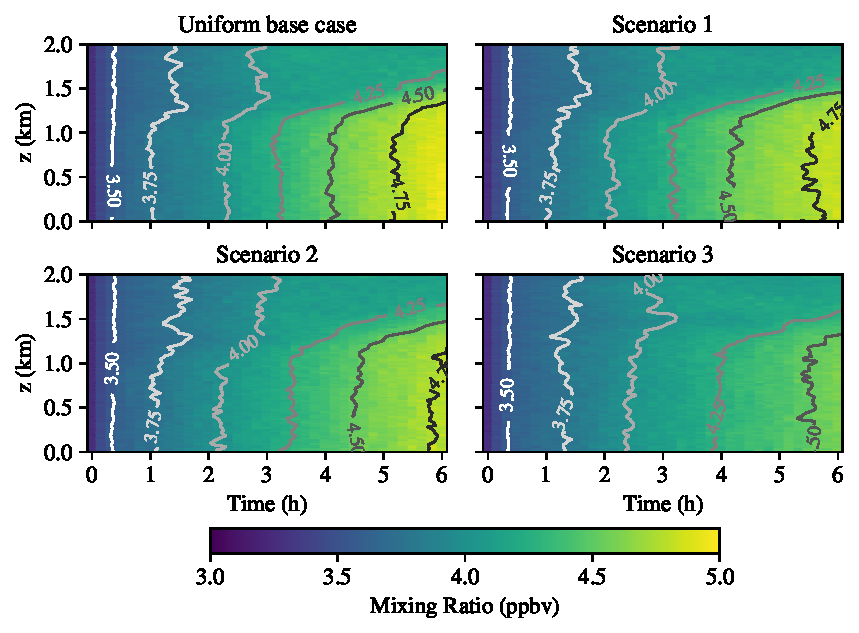
\includegraphics[width=\textwidth]{figures/chapter5/height-time-pmc_SO4-four-scenarios.pdf}
    \caption{Time-height plots for aerosol sulfate across each emissions scenario. Isopleths indicate sulfate mixing ratio in ppbv ranging from 3.5--4.75 ppbv.}
    \label{fig:ht-so4}
\end{figure}

Figure \ref{fig:ht-so4} shows time-height plots for aerosol sulfate concentrations in parts per billion by volume (ppbv). Mixing ratios are shown instead of mass concentrations as mixing ratio is independent of the atmospheric pressure and density. To compute the mixing ratio in ppbv for aerosol concentrations natively output by WRF-PartMC in \si{kg.m^{-3}}, concentrations are multiplied by the inverse of atmospheric density for each vertical level and by a factor of $10^9$ to convert from mol/mol to parts per billion.

As with previous time-height plots presented in Chapter 4, each pixel in the time-height grid mesh represents the average concentration over a given vertical level and time. Isopleths indicate lines of constant sulfate mixing ratios, ranging from 3.50 to 4.75 ppbv in increments of 0.25 ppbv.

Initially, each scenario contains a uniform sulfate concentration of $\approx3.5$ ppbv. During the first hour, concentrations gradually increase everywhere, likely due to the oxidation of ambient SO$_2$ and partitioning of resulting H$_2$SO$_4$ into the aerosol phase due to its extremely low volatility vapor pressure. As emissions turn on at $t=1$ h, the concentration of sulfate across emissions scenarios begins to diverge. In the uniform base case, sulfate concentrations steadily increase within the planetary boundary layer through $t=6$ h up to 4.75 ppbv. For high $SH$ scenarios such as scenario~3, the rate of increase in sulfate concentrations is suppressed--it takes nearly two hours for sulfate concentrations to increase from 4.25 ppbv at $t=4$ h to 4.50 by $t=6$ h whereas the same increase under the uniform base case takes approximately 1 hour between $t=3$ h and $t=4$ h. This results in lower sulfate concentrations within the planetary boundary layer under high $SH$ scenarios through $t=6$ h. For each scenario and timestep, we find that sulfate concentrations are approximately uniform throughout the planetary boundary layer. This is to be expected, as the vapor pressure of H$_2$SO$_4$ is only a weak function of temperature over the range of temperatures represented in the simulated planetary boundary layer ($\approx303$ K near the surface decreasing to $\approx293$ K at top of the planetary boundary layer).

Sulfate concentrations are lower for high emissions heterogeneity scenarios. This results from the partitioning of less H$_2$SO$_4$ into the aerosol phase. Because H$_2$SO$_4$ possesses a very low volatility vapor pressure, nearly all available H$_2$SO$_4$ will enter the aerosol to form sulfate. This indicates that the availability of sulfate is controlled by the gas phase oxidation of SO$_2$ to form H$_2$SO$_4$ via OH, and that less OH reacts with SO$_2$ under high emissions heterogeneity scenarios. 

There are numerous contributing factors which alter the availability of OH, first of which is the emissions heterogeneity of the plume. In high heterogeneity scenarios where concentrations in the emissions plume are very high, OH near the vicinity of the plume will rapidly react with the plume constituents including SO$_2$, NO$_x$, and VOCs. This quickly strips the availability of OH in the core of the plume. Reactions including photolytic processes outside the plume that produce OH are not able to replenish the concentration of OH near the plume due to an inability to mix and entrain OH into the plume fast enough. As a result, OH is chemically segregated from its reactants in the plume including SO$_2$. 

In addition to impacts of emissions plume spatial heterogeneity and chemical segregation, the availability of OH in high emissions heterogeneity scenarios may also be reduced due to lower concentrations of ozone as found in chapter 4. The photolysis of ozone into singlet oxygen and subsequent reaction with H$_2$O is an important formation mechanism for OH. 

% Nicole noted that this feedback is not included...
%In addition to the mechanism responsible for the reduction in the abundance of ozone discussed in chapter 4, it is possible that high emissions spatial heterogeneity scenarios with   significantly elevated concentration levels of both gas phase species and aerosols alters the rate of photolysis reactions due to increased optical depth in the core of the plume and  increased scattering and absorption of radiation by aerosols. 

\begin{figure}[!t]
  \centering
    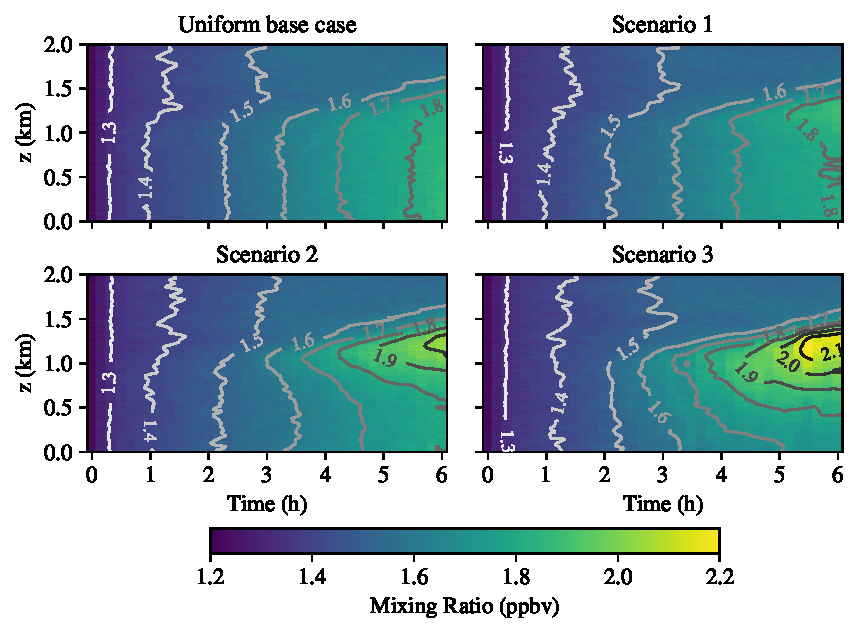
\includegraphics[width=\textwidth]{figures/chapter5/height-time-pmc_NH4-four-scenarios.pdf}
    \caption{Time-height plots for aerosol ammonium across each emissions scenario. Isopleths indicate ammonium mixing ratio in ppbv ranging from 1.3--2.1 ppbv.}
    \label{fig:ht-nh4}
\end{figure}

Time-height plots for ammonium concentrations in each emissions scenario are shown in Figure \ref{fig:ht-nh4}. Initially, aerosol ammonium concentrations are uniformly 1.2 ppbv everywhere. Ammonium concentrations steadily increase as ambient ammonia partitions into the aerosol phase. Following the release of emissions at $t=1$ h, ammonium concentrations are similar across each scenario between $t=1$ h to $t=2$ h with concentrations increasing to 1.5 ppbv. Subsequently, ammonium concentrations differ both spatially and temporally across emissions scenarios. Ammonium concentrations in the base case remain diffuse and relatively uniform throughout the planetary boundary layer, increasing to 1.8 ppbv through $t=6$ h. As $SH$ increases across scenarios, ammonium concentrations in the upper planetary boundary layer increase to as much as 2.1 ppbv in scenario~3 by $t=5$ to $t=6$ h. Meanwhile, concentrations in the lower planetary boundary layer remain near 1.7--1.8 ppbv.

\begin{figure}[!t]
  \centering
    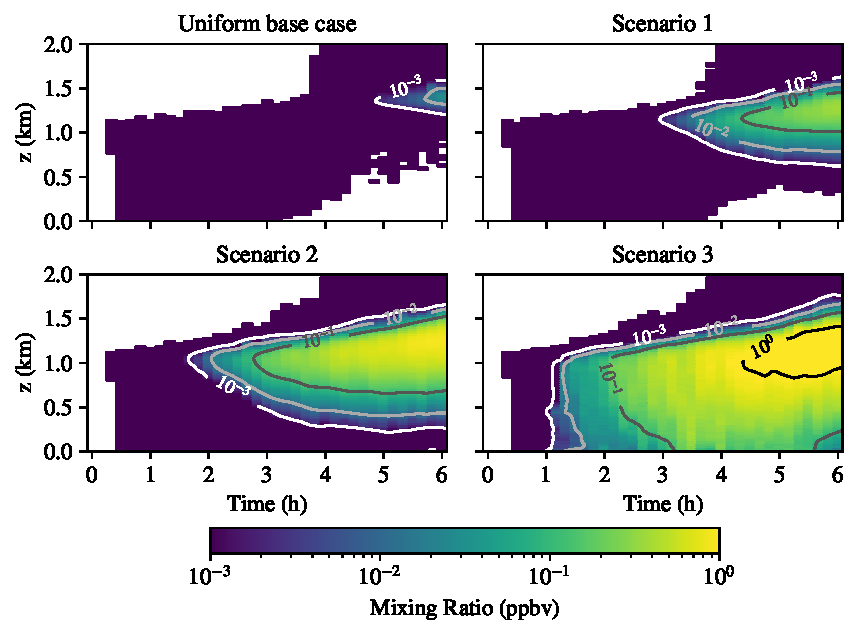
\includegraphics[width=\textwidth]{figures/chapter5/height-time-pmc_NO3-four-scenarios.pdf}
    \caption{Time-height plots for aerosol nitrate across each emissions scenario. Isopleths indicate nitrate mixing ratio in ppbv ranging from $10^{-3}$ to $10^0$ ppbv.}
    \label{fig:ht-no3}
\end{figure}

Figure \ref{fig:ht-no3} shows time-height plots of aerosol nitrate concentrations for each emissions scenario. Note the logarithmic scaling for the color bar as nitrate concentrations span numerous orders of magnitude due to trace concentrations in some regions. Initially, no nitrate is present in the aerosol phase (zero concentrations are indicated by white). Nitrate concentrations remain at or below $10^{-3}$ ppbv in the free troposphere throughout each scenario. When compared to sulfate and ammonium, the abundance of nitrate is most sensitive to emissions spatial heterogeneity as only trace amounts of nitrate ($10^{-3}$--$10^{-2}$ ppbv) are present in the upper planetary boundary layer in the uniform base case, whereas concentrations reach 1 ppbv in the upper planetary boundary layer in scenario~3. Additionally, the formation of nitrate occurs over a broader depth of the planetary boundary layer for high $SH$ scenarios and the onset of formation occurs earlier.

Both ammonium and nitrate increase in concentration with height in the planetary boundary layer due to the strong dependence of ammonium nitrate formation on temperature. Over the range of ambient temperatures observed in the boundary layer, the equilibrium dissociation constant of ammonium nitrate varies over several orders of magnitude and increases with temperature. This means that at lower temperatures conditions such as the upper planetary boundary layer, the equilibrium of ammonia and nitric acid in the gas phase will be low and the formation of ammonium nitrate in the aerosol phase is preferred. Note that nitric acid forms by reacting OH with NO$_2$. The higher concentrations of NO$_2$ observed for high emissions spatial heterogeneity scenarios in chapter 4 indicates an increase in nitric acid contingent on the availability of OH. 

Sulfate and nitrate are both anions with charge $-2$ and $-1$, respectively, while ammonium is a cation with charge +1. In turn, ammonium plays an important role in neutralizing both sulfate and nitrate. Due to the extremely low volatility of H$_2$SO$_4$, it rapidly partitions into the aerosol phase where it dissociates into SO$_4^{-2}$. In turn, available ammonia will first partition into the aerosol phase and neutralize sulfate by forming ammonium sulfate. Any remaining ammonia in excess of what is required to neutralized the sulfate, referred to as free ammonia, will enter the aerosol and bind to nitrate, thus forming ammonium nitrate. Crucially, the abundance of free ammonia determines the concentration of nitrate in the aerosol phase; if no free ammonia is available then no nitrate will enter the aerosol, whereas the presence of free ammonia allows a one-to-one molar ratio of nitrate to ammonium in the form of ammonium nitrate. Thus, the decrease in sulfate under high emissions spatial heterogeneity scenarios indicates there is more free ammonia in the aerosol which may neutralize nitric acid by forming ammonium nitrate. This helps explain why both ammonium and nitrate concentrations increase as emissions spatial heterogeneity increases. 

%\hl{Seinfeld and Pandis (10.4.4) discuss the SNA system and the two important regimes, ammonia-rich and ammonia-poor. In ammonia-poor, there isnt enough ammonia to neutralize the sulfate and most ammonia will exist in the gas phase and consequentially ammonium nitrate levels will also be low. In the ammonia rich case, there is excess ammonium than what is necessary to neutral all of the sulfate and thus the free ammonia will form ammonium nitrate.}

\begin{figure}[!t]
  \centering
    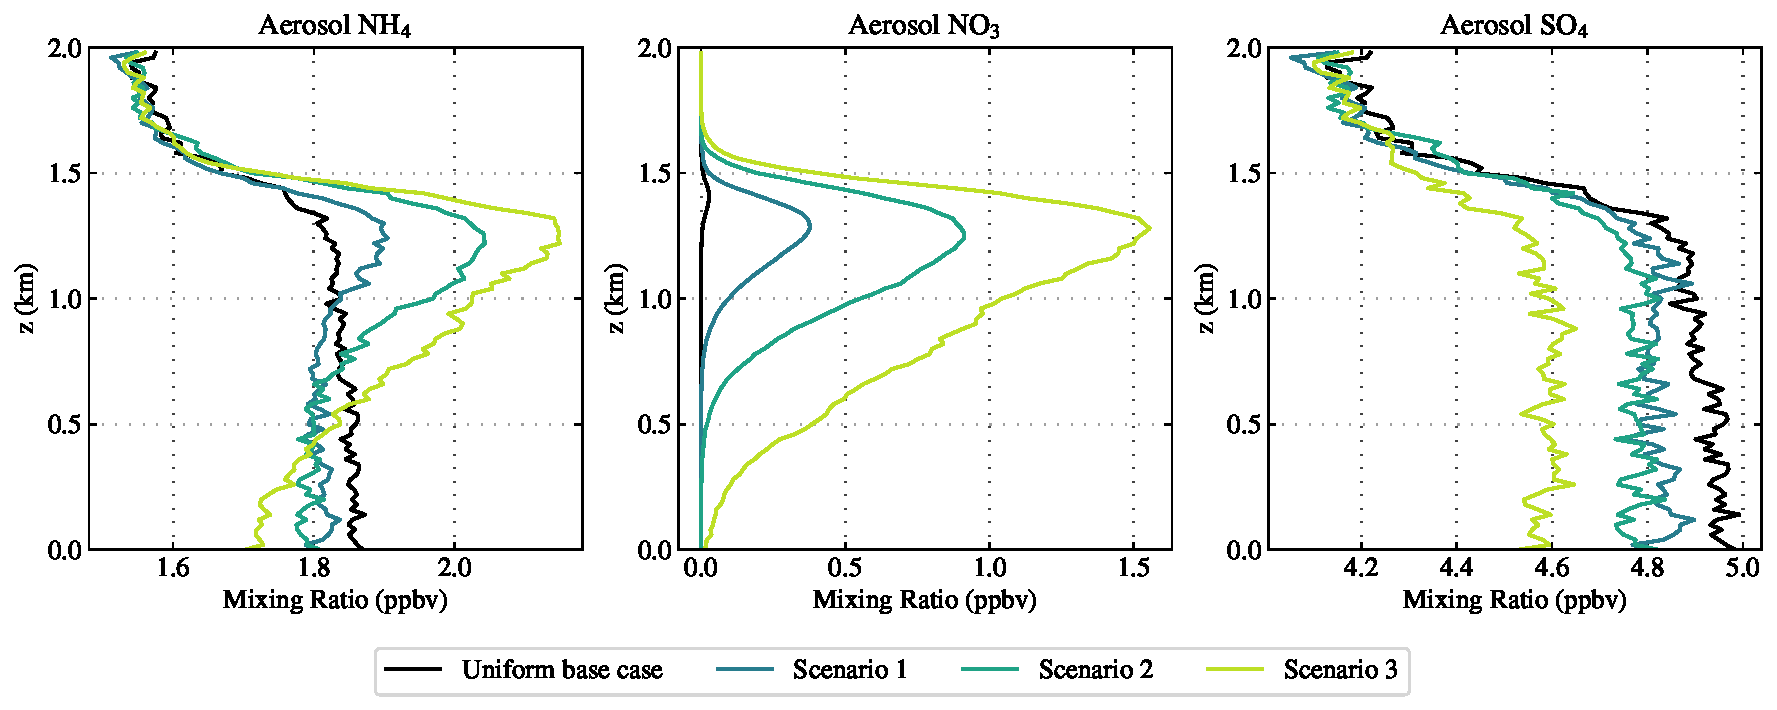
\includegraphics[width=\textwidth]{figures/chapter5/aerosol-SNA-vertical-profiles-time36.pdf}
    \caption{Vertical profiles of aerosol ammonia, nitrate, and sulfate at $t=6$ h.}
    \label{fig:sna-vertical-profile}
\end{figure}

Time-height plots for sulfate, ammonium, and nitrate capture the spatial and temporal variation of each aerosol species across each emissions scenario. However, to help quantitatively summarize and compare the relative abundances of each species, we focus here on the final state of the sulfate-nitrate-ammonium system at the end of each simulation, $t=6$ h. Figure \ref{fig:sna-vertical-profile} shows vertical profiles of ammonia, nitrate, and sulfate for $t=6$ h, whereby each vertical profile represents the horizontally averaged concentration in ppbv at each vertical level of the domain.

We find that ammonium has a relatively uniform concentration of 1.85 ppbv in the planetary boundary layer for the uniform base case. As the spatial heterogeneity of emissions scenarios increases, the abundance of ammonium increases towards the upper planetary boundary layer (which reaches a height of $z\approx1.5$~km by $t=6$ h), reaching 2.1 ppbv in the highest $SH$ scenario. Near the surface, ammonia concentrations decrease as the $SH$ of the emissions scenario increases. 

Nitrate levels increase with increasing emissions $SH$. For lower $SH$ scenarios, this increase is localized to the upper planetary boundary layer. As emissions $SH$ increases across scenarios, nitrate concentrations also increase in the lower planetary boundary layer, however the region of highest nitrate concentrations remains vertically distributed in the upper planetary boundary layer. Nitrate levels reach up to 1.5 ppbv at $z\approx1.25$~km in the highest $SH$ scenario.  

Compared with ammonium and nitrate, sulfate concentrations within the planetary boundary layer are more vertically uniform for each emissions scenario. As the $SH$ of emissions scenarios increases, sulfate concentrations are reduced by approximately the same amount everywhere in the planetary boundary layer from a planetary boundary layer average of 4.9 ppbv in the uniform base case to 4.6 ppbv in scenario~3. 

\begin{figure}[!t]
  \centering
    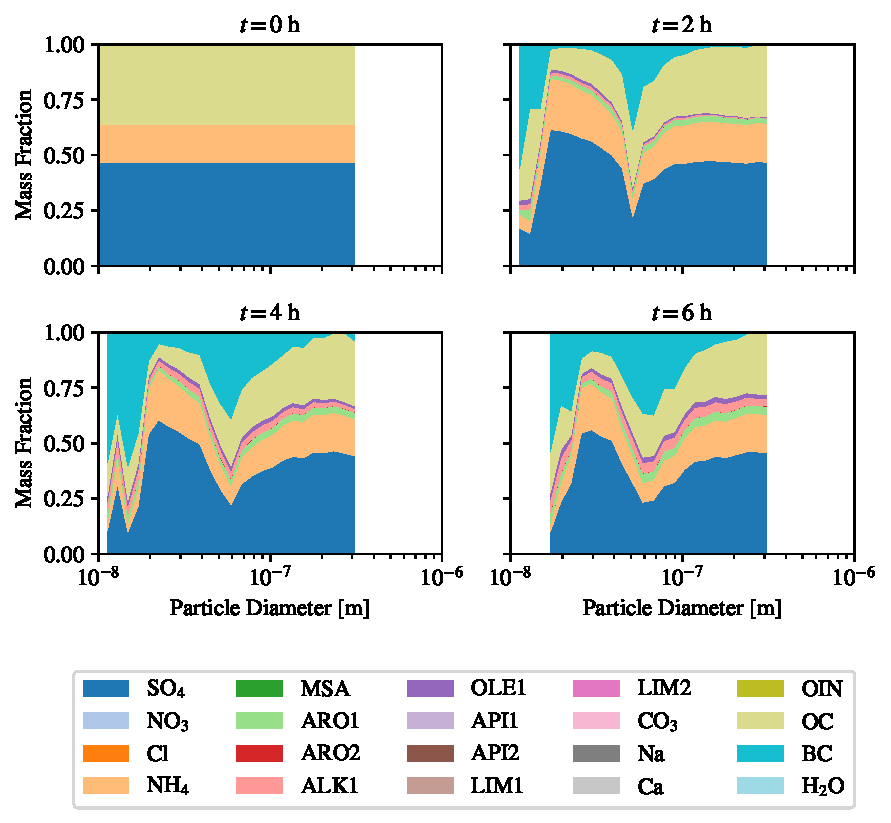
\includegraphics[width=\textwidth]{figures/chapter5/speciated-mass-frac-four-panel-uniform-basecase-z40.pdf}
    \caption{Size-resolved mass fraction for the uniform base case at regular 2-hour intervals.}
    \label{fig:mass-frac-ub}
\end{figure}

Figure \ref{fig:mass-frac-ub} shows the size-resolved mass fraction of aerosol particles in the upper planetary boundary layer ($z\approx800$ m) at 2-hour intervals for the uniform base case. The average of species mass as a fraction of aerosol total mass is displayed for each aerosol species in WRF-PartMC. As with number and mass distribution plots, species concentrations are size-resolved with 100 logarithmically spaced bins between $10^{-9}$ and $10^{-3}$ m. Mass fractions are computed by dividing the mass of each species by the total mass of a bin. In order to reduce stochastic noise, an averaging strategy similar to that utilized for the number and mass distribution plots is employed, whereby mass fractions are computed for aerosol particles contained within a 1 \si{km^2} cross section of the domain centered over the emissions plume. Aerosol species model symbols are included in the key of Figure \ref{fig:mass-frac-ub}. A comprehensive list of aerosol species in WRF-PartMC is contained in Table \ref{table:wrf-partmc-species} alongside a description of each species model symbol. 

\begin{table}[!t]
\centering
\caption{Aerosol species and associated hygroscopicities in WRF-PartMC}
\begin{tabular*}{.6\linewidth}{@{\extracolsep{\fill}} lcc}
\\[-2ex]\hline 
     \hline \\[-2ex] \textbf{Aerosol species} & \textbf{Model symbol} & \textbf{Hygroscopicity $\kappa$} \\
\midrule
Sulfate & SO4 & 0.65 \\
Nitrate & NO3 & 0.65 \\
Chloride & Cl & 1.28 \\
Ammonium & NH4 & 0.65 \\
Nethanesulfonic acid & MSA & 0.53 \\
Aromatic & ARO1 & 0.1 \\
Aromatic & ARO2 & 0.1 \\
Alkanes & ALK1 & 0.1 \\
Olefin & OLE1 & 0.1 \\
$\alpha$-pinene & API1 & 0.1 \\
$\alpha$-pinene & API2 & 0.1 \\
Limonene & LIM1 & 0.1 \\
Limonene & LIM2 & 0.1 \\
Carbonate & CO3 & 0.53 \\
Sodium & Na & 1.28 \\
Calcium & Ca & 0.53 \\
Other inorganics & OIN & 0.1 \\
Organic carbon & OC & 0.001 \\
Black carbon & BC & 0 \\
Water & H2O & 0 \\
\\[-2ex]\hline 
     \hline \\[-2ex]
\end{tabular*}
\label{table:wrf-partmc-species}
\end{table}

For the initial condition, the composition of all particles is identical, with a mixture comprised of sulfate, organic carbon (OC), and ammonium. Once emissions are active at $t=1$ h, the release of carbonaceous primary aerosol introduces black carbon (BC) into the aerosol population.  By $t=6$ h, BC makes up a meaningful fraction of aerosol mass for fine particulates; particles with diameter $\approx20$~nm are up to 50\% BC and particles near 50--60~nm are $\approx40\%$ BC.

Additionally, volatile organic compounds (VOCs) are emitted in the gas phase which are oxidized, lowering their volatility and allowing them to condense into the aerosol phase as secondary organic aerosol (SOA). SOA species are organized by functional group in WRF-PartMC and include aromatics (``ARO1", ``ARO2"), alkanes (``ALK1", ``ALK2"), limonenes (``LIM1", ``LIM2"), etc (see Table \ref{table:wrf-partmc-species} for a full list). In size-resolved mass fraction plots, SOA appears as a ribbon of green, pink, and purple atop nitrate (orange), indicating that alkanes, olefins, and aromatics comprise the bulk of SOA species present in aerosol particles. In total, SOA makes up a small fraction of aerosol mass, reaching up to 10\% of total mass by $t=6$ h.

Throughout the uniform base case simulation, the mass fraction of sulfate makes up a large portion of aerosol mass. After initially being comprised of 45\% sulfate across all aerosol diameters, by $t=6$ h, sulfate mass fraction varies between a minimum of 10\% for ultrafine particles less than 20~nm and peaks at $\approx50\%$ for particles near 30~nm. Particles in the accumulation mode are comprised of 30--40\% sulfate. Ammonium initially comprises $\approx10\%$ of aerosol mass fraction and its relative contribution to total aerosol mass is fairly consistent across time, especially for larger particles ($D_p > 0.1$~\si{\mu m}). The mass fraction of ammonium reaches a minimum for particles ultrafine particles less than 30~nm in diameter. It is important to note that no nitrate is present at any point during the uniform base case simulation.

\begin{figure}[!t]
  \centering
    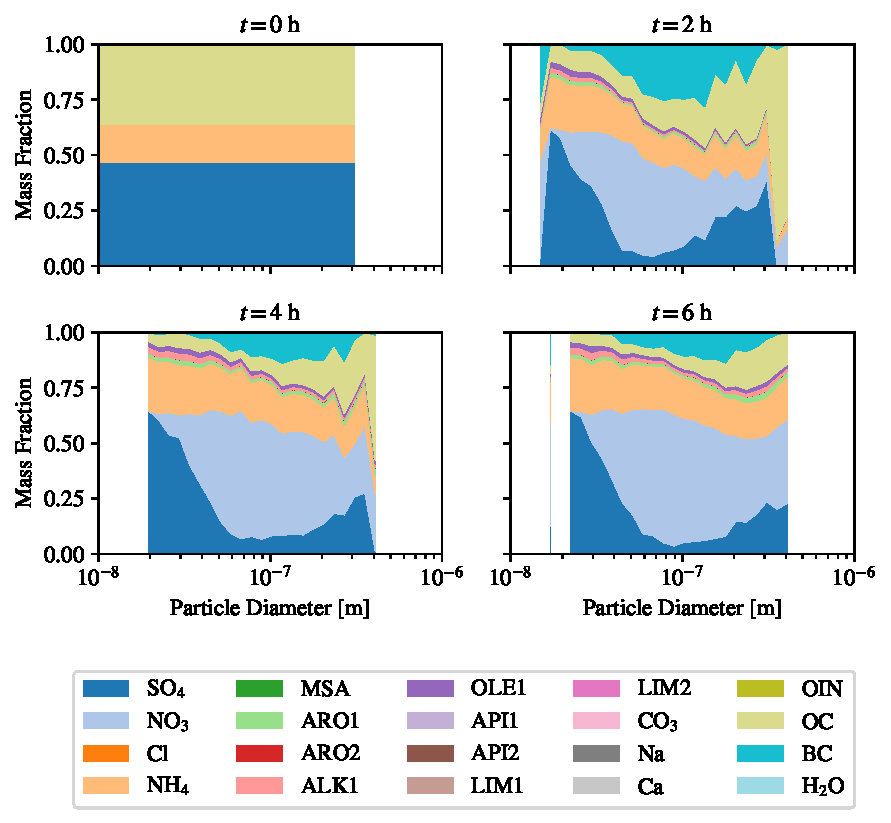
\includegraphics[width=\textwidth]{figures/chapter5/speciated-mass-frac-four-panel-point-source-1x1-z40.pdf}
    \caption{Size-resolved mass fraction for emissions scenario~3 at regular 2-hour intervals showing species mass fraction as a percent of total aerosol mass vs. particle diameter.}
    \label{fig:mass-frac-s3}
\end{figure}

Figure \ref{fig:mass-frac-s3} shows size-resolved mass fraction plots for the highest heterogeneity case, scenario~3. By $t=6$ h, the composition of aerosol particles is markedly different than in the uniform base case shown in Figure \ref{fig:mass-frac-ub}. Most notably, we find that nitrate comprises a large fraction of aerosol mass, especially for particle diameters near $D_p\approx0.1$~\si{\mu m}. As particle diameter decreases below 0.1 \si{\mu m}, the mass fraction of sulfate steady increases from less than 10\% to nearly 60\% for particles with diameter $D_p  \lesssim 30$~nm. Sulfate and nitrate effectively replace the large mass fraction of BC found for these ultrafine particles. By $t=6$ h, sulfate, nitrate, and ammonium jointly comprise a majority of aerosol mass across all particles diameters observed in emissions scenario~3. For particles smaller than 0.1 \si{\mu m}, sulfate, nitrate, and ammonium represent over 80\% of aerosol mass. For particles larger than 0.1 \si{\mu m}, these species comprise 70--80\% of aerosol mass.

Differences observed in aerosol composition are important due to the varying properties of aerosol species and their downstream influence on the atmospheric state. For example, particle hygroscopicity determines the critical supersaturation at which a particle of a given diameter will active as a cloud condensation nucleus. Hygroscopicity is parameterized using the $\kappa$-Köhler theory of \textcite{petters_single_2007}. $\kappa$-Köhler theory is a modification to Köhler's relationship for determining the saturation ratio over a particle and the critical supersaturation at which the particle activates \parencite{kohler_nucleus_1936}. Each aerosol species has an associated hygroscopicity $\kappa$, and the total particle $\kappa$ is a volume-weighted sum of each species $\kappa$. Note that Table \ref{table:wrf-partmc-species} lists the hygroscopicity parameter $\kappa$ of each aerosol species and is highly variable (e.g., the hygroscopicity of BC is zero while sulfate has a hygroscopicity of 0.65). Values of  $\kappa$ greater than 0.5 indicate the aerosol species has a high hygroscopicity, while $\kappa=0$ corresponds to a nonhygroscopic compound.

\begin{figure}[!t]
  \centering
    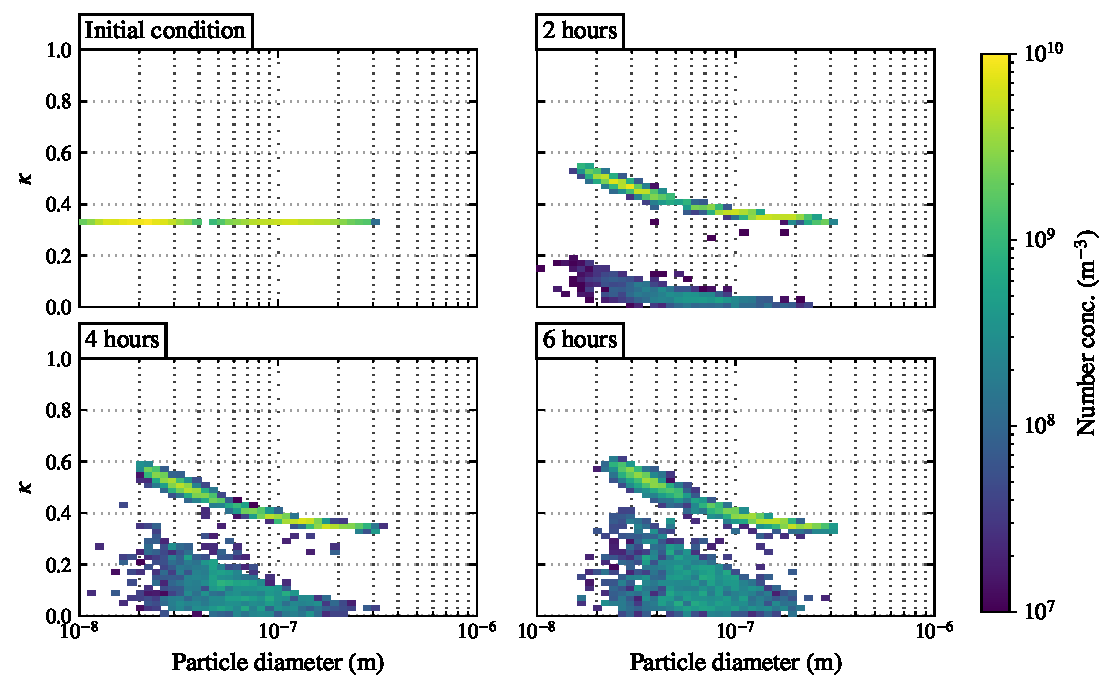
\includegraphics[width=\textwidth]{figures/chapter5/2d-kappa-dist-4-panel-uniform-basecase-z40.pdf}
    \caption{2-dimensional number distributions $n(D_p, \kappa)$ at regular two-hour intervals for the uniform base case.}
    \label{fig:2d-kappa-dist-ub}
\end{figure}

Figure \ref{fig:2d-kappa-dist-ub} shows two-dimensional number distributions at regular two hour intervals for the uniform base case in the upper planetary boundary layer ($z\approx800$ m). The x-axis indicates particle diameter in meters, while hygroscopicity $\kappa$ is plotted along the y-axis. Particles are binned into a two-dimensional histogram by diameter (50 bins from 10~nm to 1~$\mu$m) and $\kappa$ (50 bins from 0 to 1) and the number concentration within each bin is tallied and displayed as a colorbar. Bins with zero particles are filled in white.

At the initial condition, we find that all particles posses the same total hygroscopicity, $\kappa=0.32$, as each is a mixture of ammonium sulfate and OC. Beginning at $t=1$ h, emissions of primary aerosol and gas phase species alter the distribution of particle hygroscopicity. Recall that emitted primary aerosol are composed of OC and BC with $\kappa$ values 0.001 and 0, respectively. This results in a distribution of low-$\kappa$ aerosol particles situated beneath the sulfate-rich aerosol. As the simulation evolves, gas-particle partitioning and coagulation age the aerosol population, increasing particle hygroscopicity.

\begin{figure}[!t]
  \centering
    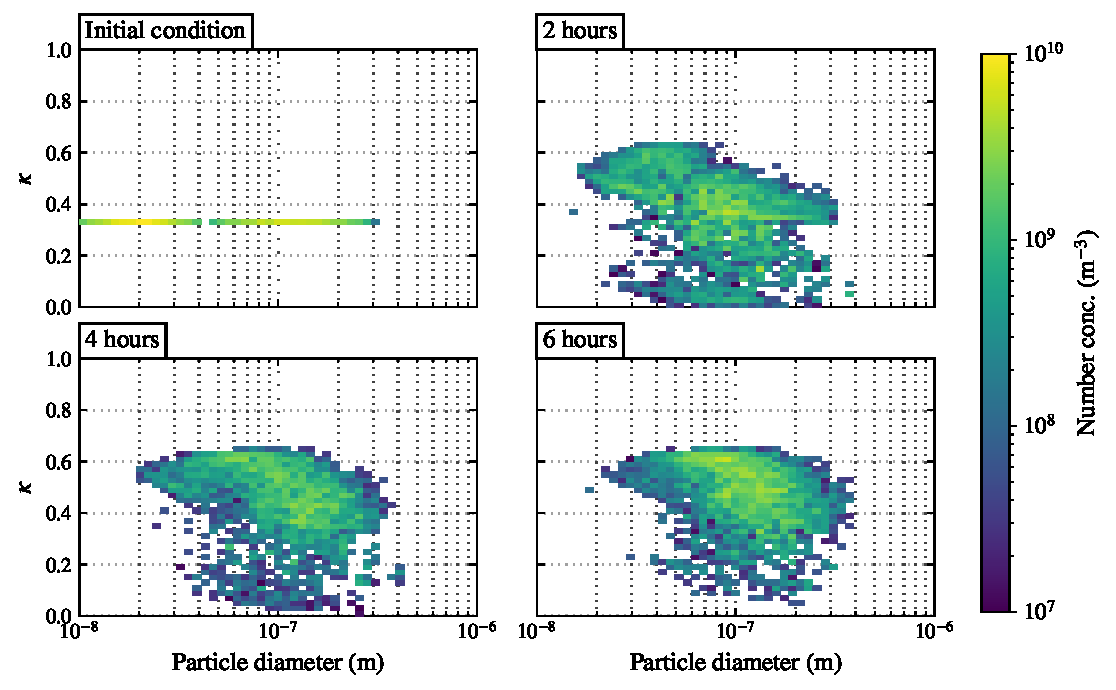
\includegraphics[width=\textwidth]{figures/chapter5/2d-kappa-dist-4-panel-point-source-1x1-z40.pdf}
    \caption{2-dimensional number distributions $n(D_p, \kappa)$ at regular two-hour intervals for scenario~3.}
    \label{fig:2d-kappa-dist-s3}
\end{figure}

Figure \ref{fig:2d-kappa-dist-s3} shows two-dimensional size distributions at regular two hour intervals for the highest $SH$ scenario, scenario~3. We find that following the initial condition, the evolution of the $\kappa$-resolved size distribution differs markedly from the uniform base case in numerous ways. First, the abundance of low-$\kappa$ primary aerosol due to emissions is greatly reduced for $t=2$ h to $t=6$ h. The increased rate of coagulation for high $SH$ scenarios shown in Section \ref{ideal-coag-results} and the removal of Aitken model particles via the size-dependent nature of coagulation discussed in Section \ref{size-dists} jointly indicate that coagulation is responsible for removing  low-$\kappa$ aerosol particles in the high-concentration emissions plume. Additionally, we find a greater abundance of high-$\kappa$ particles in the size range 20~nm to 0.4 \si{\mu m} with $\kappa$ in excess of 0.6 for some particles near $D_p=0.1$~\si{\mu m}. By comparison, far fewer particles in the uniform base case possess $\kappa\approx0.6$ and are limited to the size range 20--30~nm. 

\subsection{Aerosol mixing state}

\begin{figure}[!t]
  \centering
    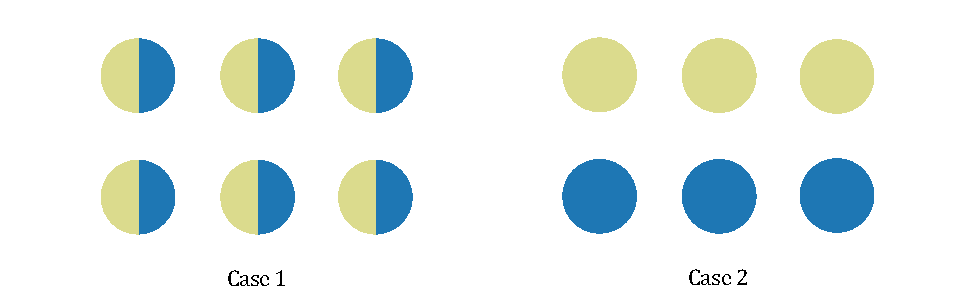
\includegraphics[width=\textwidth]{figures/chapter5/mixing-state-ideal-cases.pdf}
    \caption{Two idealized cases for aerosol populations composed of ammonium sulfate (blue) and organic carbon (beige). Case 1 is fully internally mixed while case 2 is fully externally mixed, yet each case contains the same bulk concentration of each species.}
    \label{fig:mixing-state-scenarios}
\end{figure}

So far in this section we have shown results for the bulk and size-resolved composition of the aerosol. That is, we have shown which aerosol species are contained in the population, their mean abundances, and how they vary with particle size. However, these results do not indicate how each aerosol species is distributed amongst the particles in the population. Consider two cases for aerosol populations shown in Figure \ref{fig:mixing-state-scenarios}, each with a grouping of six monodisperse aerosol particles. In the first case, all aerosol particles are an equal mixture of 50\% ammonium sulfate and 50\% OC. In the second case, half of the particles are 100\% ammonium sulfate and the remaining half are 100\% OC. When averaged to find the bulk composition of the population, each case leads to the same conclusion--the population is composed of 50\% ammonium sulfate and 50\% OC. However, this bulk state oversimplifies the compositional diversity of the particle population and aerosol particle properties vary considerably across each case. Note that the hygroscopicity $\kappa$ of each particle differs across both cases. If all particles are internally mixed as in the first case (i.e., each particle is a mixture of ammonium sulfate and OC), the hygroscopicity of all particles will be $\kappa=0.33$. For the second case, the particles are externally mixed (i.e., each particle is purely composed of a single aerosol species), resulting in the ammonium sulfate particles being highly hygroscopic, $\kappa=0.65$, while the pure OC particles are nearly nonhygroscopic, $\kappa=0.001$. As a consequence, there will exist a supersaturation at which all of the particles in case 1 active as CCN, while only half of the particles in the second case will active. This illustrates the importance of the aerosol mixing state, which describes how externally or internally mixed aerosol species are in the particle population. 

The mixing state $\chi$ is quantified using the metric definition of \textcite{riemer_quantifying_2013} and is defined as 
\begin{equation}
\chi = \frac{D_{\alpha}-1}{D_{\gamma}-1},
\end{equation}
where $D_{\alpha}$ is the average particle species diversity and $D_{\gamma}$ is the bulk population species diversity. $D_{\alpha}$ is related to the average Shannon entropy for each particle as 
 \begin{equation}
D_{\alpha} = \exp\left(\sum_{i=1}^N p_i H_i\right),
\end{equation}
where $p_i$ is the mass fraction of particle $i$ in the population and $H_i$, the Shannon entropy of the species distribution in particle $i$, is 
\begin{equation}
H_i = \sum_{a=1}^A -p_i^a\ln(p_i^a),
\end{equation}
where $p_i^a$ is the mass fraction of species $a$ in particle $i$.

$D_{\gamma}$ is related to the Shannon entropy for the distribution of an aerosol species in the population as 
 \begin{equation}
D_{\gamma} = \exp\left(\sum_{a=1}^A p^a \ln(p^a)\right),
\end{equation}
where $p^a$ is the mass fraction of species $a$ in the population.

\begin{figure}[!t]
  \centering
    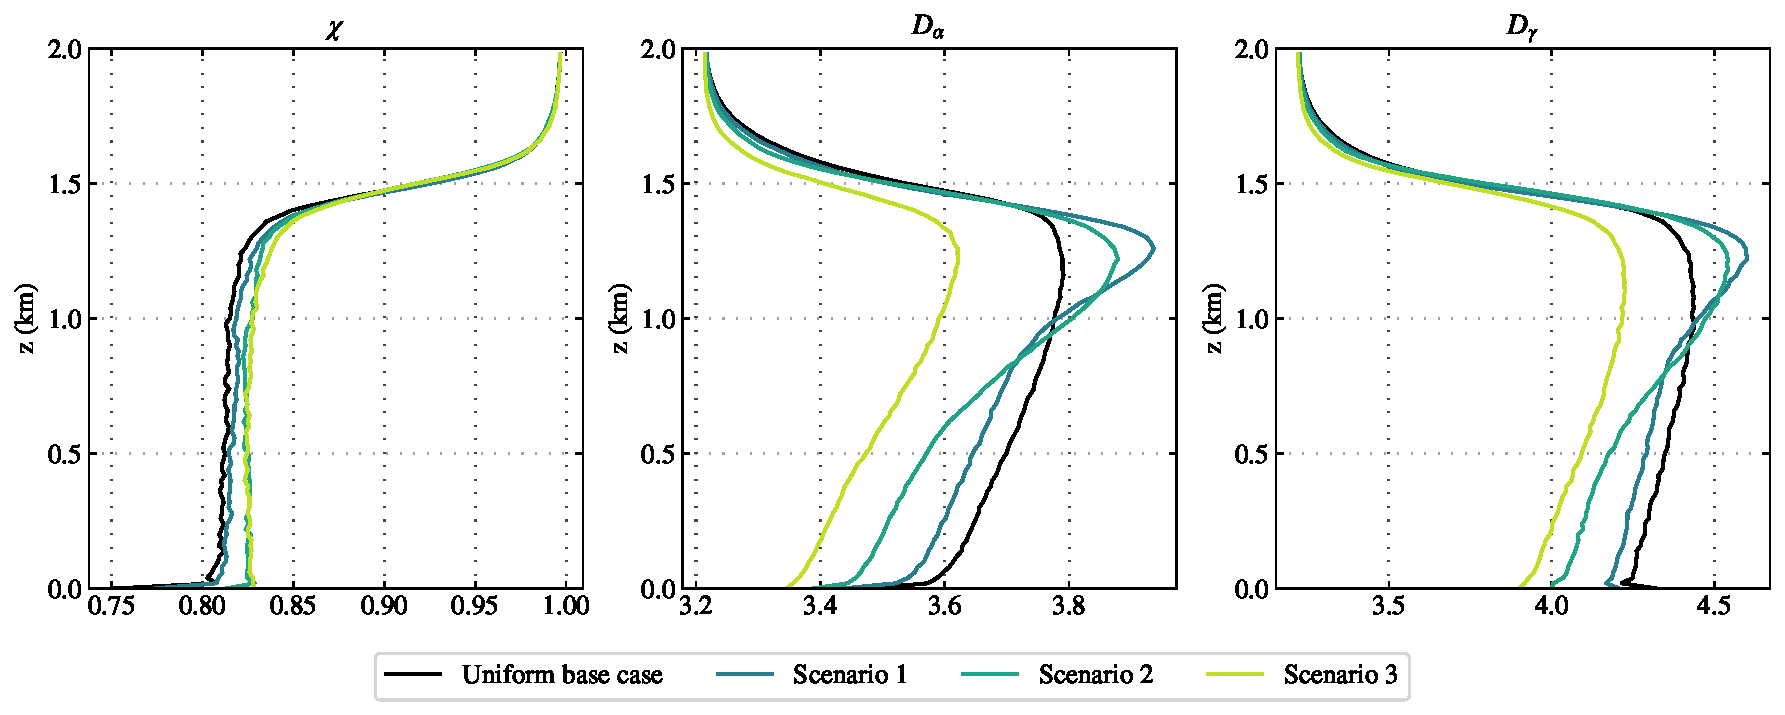
\includegraphics[width=\textwidth]{figures/chapter5/aerosol-mixingstate-vertical-profiles-time36.pdf}
    \caption{Vertical profiles for mixing state $\chi$ and diversity measures $D_{\alpha}$ and $D_{\gamma}$ for each emissions scenario at $t=6$ h.}
    \label{fig:mixing-state-vert-profiles}
\end{figure}

Figure \ref{fig:mixing-state-vert-profiles} shows vertical profiles for $\chi$ and its associated diversity measures $D_{\alpha}$ and $D_{\gamma}$ for each emissions scenario at $t=6$ h. We find that $\chi$ is approximately the same across each emission scenario in both the planetary boundary layer and in the free troposphere. Furthermore, $\chi$ is nearly uniform within the planetary boundary layer, with values near $\chi\approx0.81$ in the uniform base case and $\chi\approx0.83$ in the highest $SH$ scenario, scenario~3. Above the planetary boundary layer, $\chi$ matches closely across all scenarios and reaches $\chi\approx1$ by the top of the domain. These results point to a near-fully internally mixed aerosol population in the planetary boundary layer and completely internally mixed aerosol above the planetary boundary layer. 

We find that diversity measures $D_{\alpha}$ and $D_{\gamma}$ increase with height in the planetary boundary layer and subsequently decrease in the free troposphere. In the middle to lower planetary boundary layer, both $D_{\alpha}$ and $D_{\gamma}$ decrease for high $SH$ scenarios relative to the uniform base case. We find that $D_{\alpha}$ and $D_{\gamma}$ both peak near the top of the planetary boundary layer and reach a maximum for emissions scenario~1 at 3.95 and 4.6, respectively. 

$D_{\alpha}$ and $D_{\gamma}$ are lower near the surface due to the presence of freshly emitted primary aerosol which are a mix of primary organic aerosol and black carbon (resulting in a maximum value of 2 for $D_{\alpha}$ and $D_{\gamma}$ of freshly emitted aerosol). As emitted aerosol rise throughout the planetary boundary layer, the particles undergo aging due to coagulation events and gas-particle partitioning which increase the average number of species within particles and across the population. The inversion layer capping the planetary boundary layer prevents the transfer of aged and emitted aerosol into the free troposphere. This results in  $D_{\alpha}$ and $D_{\gamma}$ near 3 in the upper domain, which is consistent with the initial condition (a mixture of ammonium sulfate and primary organic aerosol) comprised of 3 aerosol species.  

\begin{figure}[!t]
  \centering
    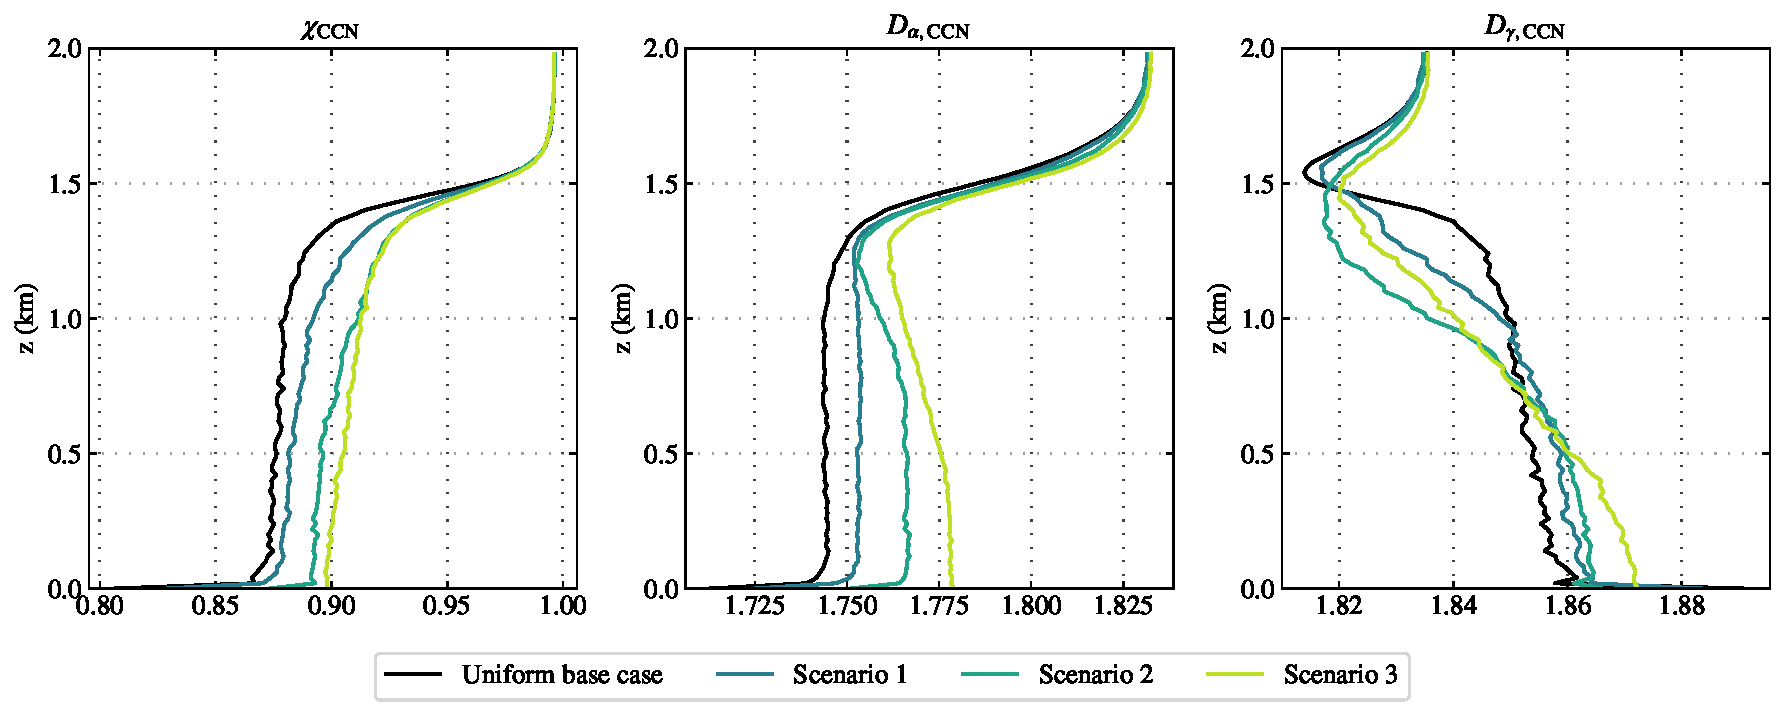
\includegraphics[width=\textwidth]{figures/chapter5/aerosol-ccn-mixingstate-vertical-profiles-time36.pdf}
    \caption{Vertical profiles for CCN mixing state $\chi_{\text{CCN}}$ and diversity measures $D_{\alpha,\text{CCN}}$ and $D_{\gamma,\text{CCN}}$ for each emissions scenario at $t=6$ h.}
    \label{fig:ccn-mixing-state-vert-profiles}
\end{figure}

Figure \ref{fig:ccn-mixing-state-vert-profiles} shows vertical profiles for $\chi$ and diversity measures $D_{\alpha}$ and $D_{\gamma}$ for particles where species are grouped into hydrophobic (BC and OC) and hydrophilic compounds (all remaining species). This gives a measure of the CCN mixing state, referred to as $\chi_{\text{CCN}}$. Due to the use of two species groupings, $D_{\alpha,\text{CCN}}$ and $D_{\gamma,\text{CCN}}$ range between 1 (purely hydrophobic or hydrophillic) and 2 (an equal mixture of hydrophobic and hydrophillic compounds). For each emissions scenario, $\chi_{\text{CCN}}$ gradually increases in the planetary boundary layer. $\chi_{\text{CCN}}$ is slightly greater than $\chi$ for each scenario, indicating that CCN are very well mixed and composed of both hydrophillic and hydrophobic species in the planetary boundary layer. Furthermore, $\chi_{\text{CCN}}$ increases slightly with greater emissions $SH$ (e.g., at $z=500$ m, $\chi_{\text{CCN}} = 0.87$ for the uniform base case and $\chi_{\text{CCN}} = 0.90$ for scenario~3). As $SH$ increases, $D_{\alpha,\text{CCN}}$ also slightly increases in the planetary boundary layer (e.g., at $z=500$ m, $D_{\alpha,\text{CCN}} = 1.74$ for the uniform base case and $D_{\alpha,\text{CCN}} = 1.77$ for scenario~3). Above the planetary boundary layer, $D_{\alpha,\text{CCN}}$ tends to converge across emissions scenarios, increasing to $\approx1.83$ at $z=2$~km. We find that $D_{\gamma,\text{CCN}}$ gradually decreases moving vertically in the planetary boundary layer for each emissions scenario. As $SH$ increases across emissions scenarios, $D_{\gamma,\text{CCN}}$ takes on higher values in the lower to middle boundary layer, while in the middle to upper boundary layer this trend is reversed, with higher $SH$ indicating lower values of $D_{\gamma,\text{CCN}}$. 

\subsection{Impacts of emissions $SH$ on CCN activity}

We have shown that emissions spatial heterogeneity alters the aerosol composition, producing more nitrate-rich particles and that this results in an increase in aerosol hygroscopicity $\kappa$. The critical supersaturation at which a particle activates as a cloud condensation nucleus is a function of $\kappa$ and particle diameter. Thus, changes to the aerosol properties such as composition and hygroscopicity will propagate to changes in CCN activity. 

Here, we group particles by critical saturation into CCN that activate at the following supersaturation levels:  $S=0.1, 0.3, 0.6, 1.0\%$. CCN concentrations at each supersaturation level are determined in the following manner. First, the critical supersaturation $S_c$ is determined for each particle by using a root finding algorithm to solve for the critical point of the supersaturation curve $S(D_p, \kappa)$ of $\kappa$-Köhler theory \parencite{petters_single_2007}. Particles are then grouped by supersaturation ($0.1, 0.3, 0.6, 1.0\%$) required for activation in a cumulative manner (i.e., particles activating at $S=0.3\%$ are included in bins for $S=0.5\%$ and higher supersaturations as they will activate at any supersaturation higher than $S=0.3\%$). Subsequently, the concentration of CCN at each supersaturation level is determined for each grid cell. 

\begin{figure}[!t]
  \centering
    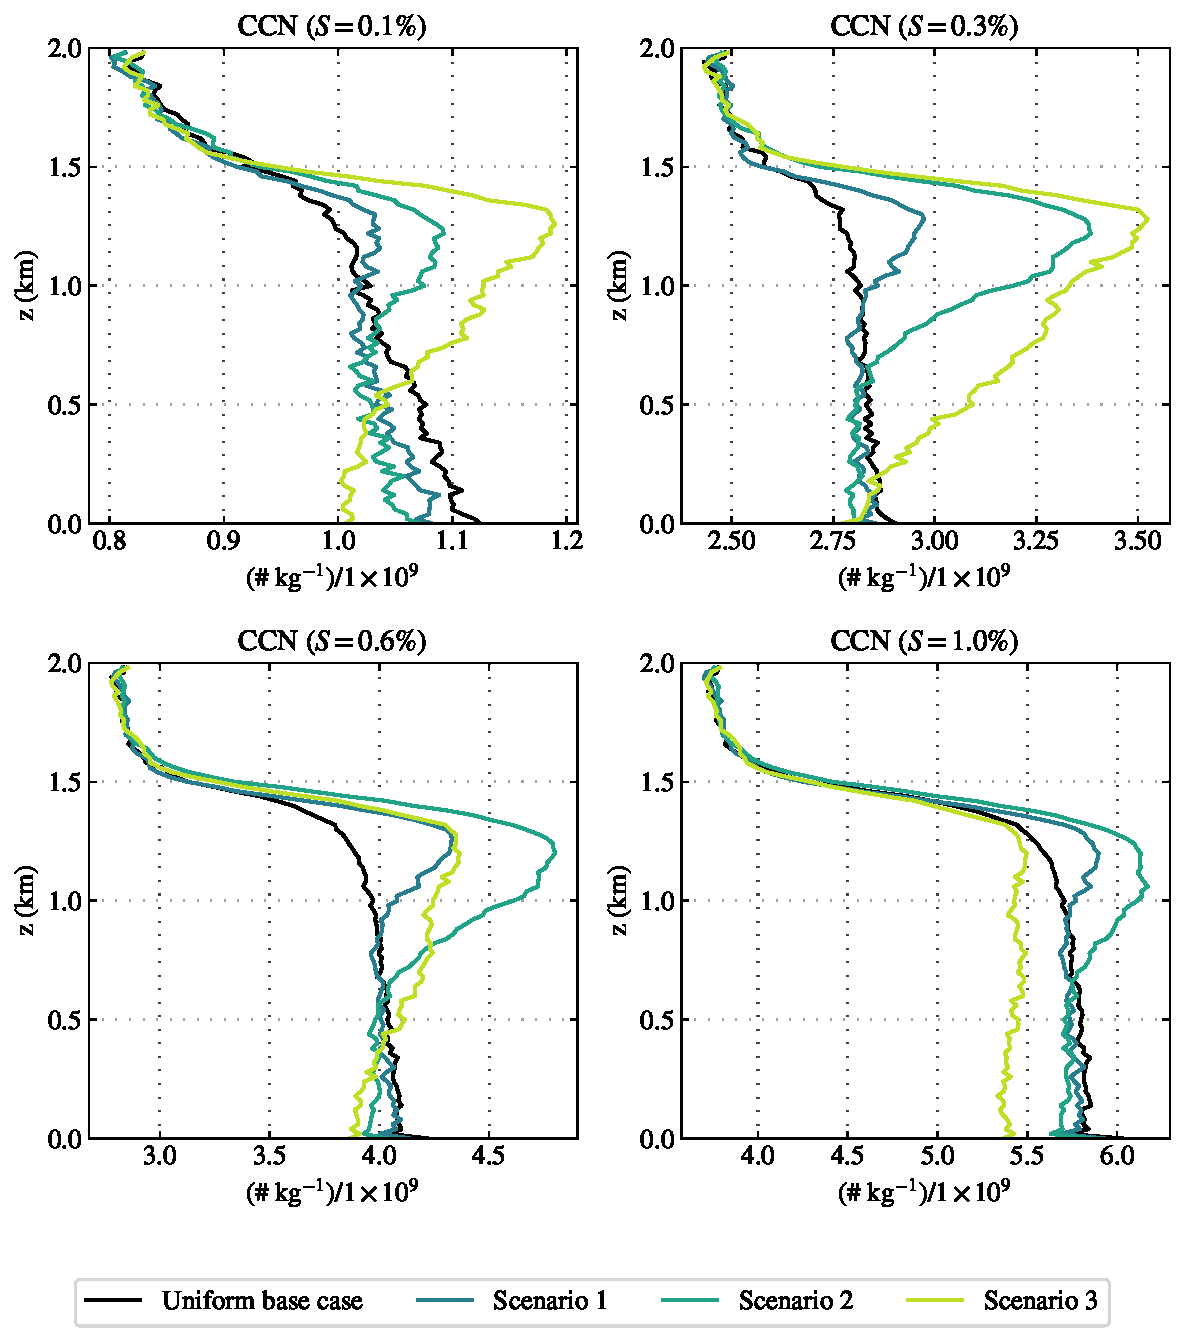
\includegraphics[width=.9\textwidth]{figures/chapter5/aerosol-ccn-vertical-profiles-time36.pdf}
    \caption{Vertical profiles ($t=6$ h) for each emission scenario of CCN activating at supersaturations $S=0.1, 0.3, 0.6, 1.0$\%}
    \label{fig:vertprof-ccn}
\end{figure}

Figure \ref{fig:vertprof-ccn} shows vertical profiles for each emissions scenario of CCN that activate at supersaturations $S=0.1, 0.3, 0.6, 1.0\%$. Each vertical profile is taken at time $t=6$ h and displays the level-averaged number concentration in number of particles per kilogram of dry air for particles that would act as CCN at each supersaturation level (note, environmental conditions do not exceed 100\% RH at any point or time in each simulation). 

For $S=0.1\%$, we find that CCN concentrations decrease with increasing $SH$ in the lower boundary layer. In the middle to upper boundary layer, the opposite trend is observed, with CCN concentrations increasing as emissions $SH$ increases. This increase is most pronounced at the top of the planetary boundary layer ($z\approx 1.25$~km), where CCN concentrations reach nearly $1.2\cdot10^{9}$~\#~\si{kg^{-1}} for scenario~3 compared to $1.0\cdot10^{9}$~\#~\si{kg^{-1}} in the uniform base case. 

Increases in CCN concentrations due to increasing emissions $SH$ are observed everywhere in the planetary boundary layer for $S=0.3\%$, with concentrations again peaking near the top of the boundary layer. For the highest $SH$ scenario, we find CCN concentrations in the upper planetary boundary layer exceed $3.5\cdot10^{9}$~\#~\si{kg^{-1}}, while in the uniform base case, CCN concentrations are a vertically uniform $2.8\cdot10^{9}$~\#~\si{kg^{-1}}. 

For $S=0.6\%$, we find that CCN concentrations in the lowest 500 m of the planetary boundary layer for Scenarios 1--3 are slightly lower than in the uniform base case. In the middle to upper planetary boundary layer, we find that the increases in $SH$ correspond to non-monotonic changes in CCN concentrations (i.e., CCN concentrations do not appear to increase with progressively higher $SH$ scenarios as found in the upper planetary boundary layer for $S=0.1\%$ and $S=0.3\%$). Instead, CCN concentrations in the upper planetary boundary layer for $S=0.6\%$ are highest for the mid-$SH$ scenario (scenario~2), followed by scenario~3, scenario~1, and the uniform base case. 

For $S=1.0\%$ we also find a complex set of responses to CCN concentrations across emissions $SH$ scenarios. For low to mid-$SH$ scenarios 1 and 2, we find that CCN concentrations in the lowest $600$ m of the planetary boundary layer closely align with the uniform base case. In the middle to upper boundary layer, scenarios 1 and 2 exhibit an increase in CCN concentrations relative to the uniform base case. We find that CCN concentrations for $S=1.0\%$ in the highest $SH$ scenario, scenario~3, are approximately uniform throughout the extent of the planetary boundary layer at $4.4\cdot10^{9}$~\#~\si{kg^{-1}}, slightly less than the $4.6\cdot10^{9}$~\#~\si{kg^{-1}} observed for the uniform base case. 

\begin{figure}[!t]
  \centering
    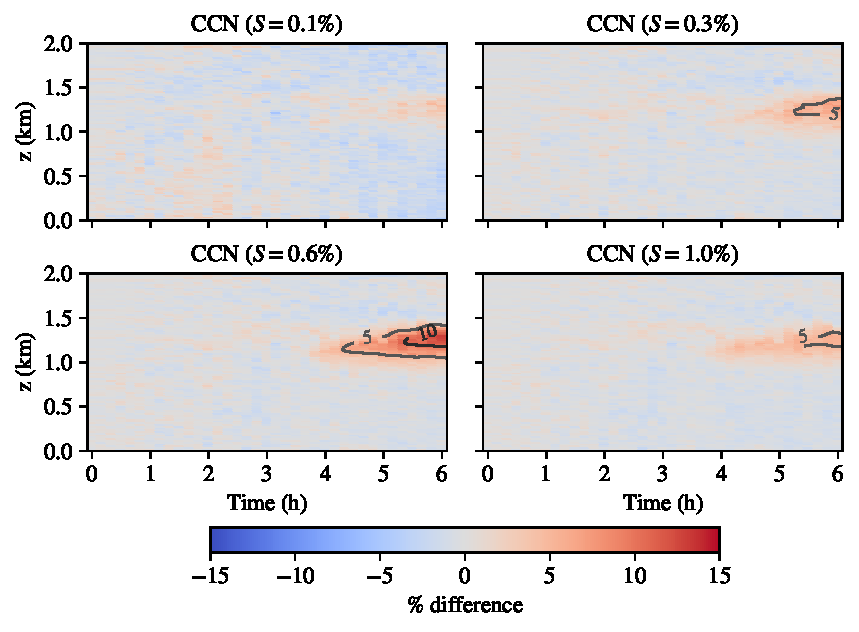
\includegraphics[width=\textwidth]{figures/chapter5/height-time-ccn-pdiff-fx1fy0.pdf}
    \caption{Time-height plots for the percent difference between CCN concentrations in the uniform base case and scenario~1 for each supersaturation level. Red indicates an increase in CCN relative to the base case while blue indicates a decrease. Isopleths indicate lines of constant percent difference in increments of 5\%.}
    \label{fig:ht-ccn-pdiff-s1}
\end{figure}

Figure \ref{fig:ht-ccn-pdiff-s1} shows time-height plots for the percent difference of CCN concentrations in emissions scenario~1 relative to the uniform base case. Plots are shown for each supersaturation level ($S=0.1, 0.3, 0.6, 1.0\%$). Red indicates increases in CCN concentrations relative to the base case while blue indicates a decrease. To aid interpretability, isopleths indicating percent difference in steps of $5\%$ are shown on each figure. If no isopleths are present, this indicates that percent difference did not exceed $5\%$ anywhere or at any time between the emissions scenario CCN concentrations and the uniform base case. Percent difference is calculated as 
\begin{equation}
    \% \text{ difference} = 100\times\left(\frac{\overline{[\text{CCN}]}(t, z, S)_{\text{Scenario}} - \overline{[\text{CCN}]}(t, z, S)_{\text{Base case}}}{\overline{[\text{CCN}]}(t, z, S)_{\text{Base case}}}\right),
\end{equation}
where $\overline{[\text{CCN}]}(t, z,S)_{\text{Scenario}}$ is the horizontally averaged concentration of CCN at time $t$ and vertical level $z$ that activate at supersaturation $S$ for the given emissions scenario and $\overline{[\text{CCN}]}(t, z, S)_{\text{Base case}}$ is the horizontally averaged concentration of CCN at time $t$ and vertical level $z$ that activate at supersaturation $S$ for the uniform base case.

Stepping through each supersaturation level, we find that at $S=0.1\%$, percent difference does not exceed 5\% at any point during the simulation. Slight spatial and temporal fluctuations are found in CCN concentrations, however, these do not appear to significantly depart from percent difference between scenario~1 and the uniform base case in the first hour of the simulation during which the configuration and spinup of each simulation is identical, indicating that internal variability due to stochastic noise is likely on the order of 1--2\%.

For $S=0.3\%$, we find a slight increase in CCN concentrations beginning at $t=5$ h from $z\approx1.1$~km to $z\approx1.4$~km on the order of 5\%. Similarly for $S=0.6\%$ and $S=1.0\%$, we find that CCN concentrations increase in the upper planetary boundary layer. At $S=0.6\%$ CCN concentrations increase up to 10\% by $t=5$ h. At $S=1.0\%$, we find similar behavior in the percent difference for $S=0.3\%$, with an increase in CCN concentrations the upper planetary boundary layer of up to 5\%.

\begin{figure}[!t]
  \centering
    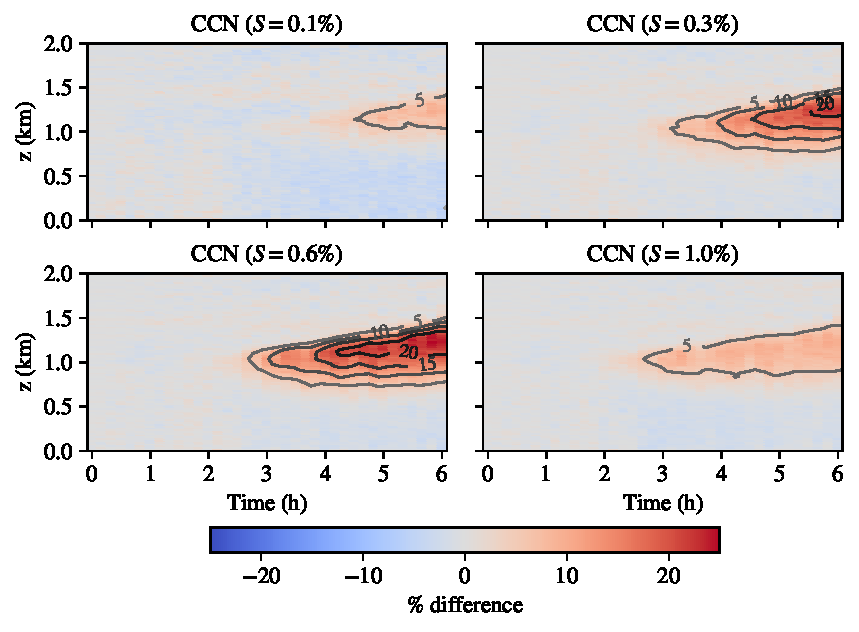
\includegraphics[width=\textwidth]{figures/chapter5/height-time-ccn-pdiff-road-10x.pdf}
    \caption{Time-height plots for the percent difference between CCN concentrations in the uniform base case and scenario~2 for each supersaturation level. Red indicates an increase in CCN relative to the base case while blue indicates a decrease. Isopleths indicate lines of constant percent difference in increments of 5\%.}
    \label{fig:ht-ccn-pdiff-s2}
\end{figure}

Figure \ref{fig:ht-ccn-pdiff-s2} shows time-height plots for percent difference in CCN concentrations at each supersaturation level between scenario~2 and the uniform base case. We find that for each supersaturation level, CCN concentrations increase in the upper planetary boundary layer by at least 5\%. Additionally, the onset of increased CCN concentrations relative to the uniform base case is earlier than found for scenario~1 for each supersaturation level. 

For $S=0.1\%$, we find that CCN concentrations in the upper planetary boundary layer increase up to 5\% beginning at $t=4.5$ h. For $S=0.3\%$ and $S=0.6\%$, we find increases of up to 20\% with elevated concentrations relative to the uniform base case beginning at $t\approx3$ h and gradually increasing in the upper planetary boundary layer through the remainder of each simulation. For $S=1.0\%$, CCN concentrations increase in a similar manner to those found for $S=0.1\%$ with concentrations increasing up to 5\% in the upper planetary boundary layer. However, CCN concentrations increase earlier than in the lower supersaturation case, with elevated concentrations by 5\% in the upper planetary boundary layer appearing around $t=2.5$ h.

\begin{figure}[!t]
  \centering
    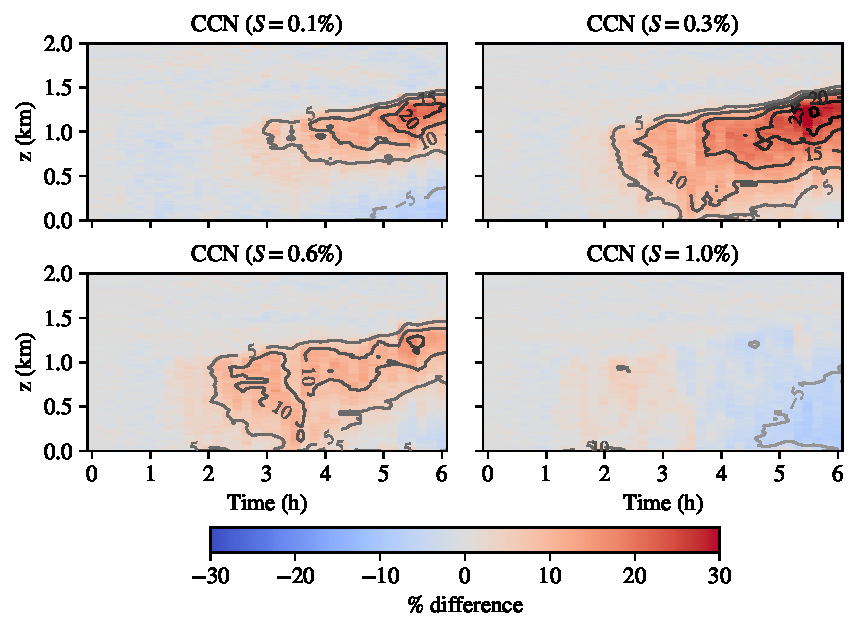
\includegraphics[width=\textwidth]{figures/chapter5/height-time-ccn-pdiff-point-source-1x1.pdf}
    \caption{Time-height plots for the percent difference between CCN concentrations in the uniform base case and scenario~3 for each supersaturation level. Red indicates an increase in CCN relative to the base case while blue indicates a decrease. Isopleths indicate lines of constant percent difference in increments of 5\%.}
    \label{fig:ht-ccn-pdiff-s3}
\end{figure}

Figure \ref{fig:ht-ccn-pdiff-s3} displays time-height plots for percent difference in CCN concentrations at each supersaturation level between scenario~3 and the uniform base case. 
Compared with scenarios 1 and 2, the trend of increasing CCN concentrations is much more vertically and temporally vaired, particularly for $S=0.3\%$ and $S=0.6\%$ where an increase in CCN concentrations begins in the upper planetary boundary layer at $t=2$ h, extends downward throughout the vertical extent of the planetary boundary layer by $t=3$ h, and moves back upwards towards the mid to upper planetary boundary layer beginning at $t=4$ h. 

For $S=0.1\%$, CCN concentrations increase by up to 20\% in the upper boundary layer by $t=5.5$ h. Beginning around $t=5$ h, CCN concentrations decrease by up to 5\% in the lowest 300 m of the domain. At $S=0.3\%$, CCN concentrations increase by up to 25\% in the upper planetary boundary layer beginning at $t=5$ h. This is the highest magnitude CCN concentration percent difference observed for any supersaturation and across any emissions scenario. For $S=0.6\%$, CCN concentrations increase by 10--15\%, indicating a notable drop in the magnitude of elevated CCN concentrations when compared to scenario~2 results for $S=0.6\%$ shown in Figure \ref{fig:ht-ccn-pdiff-s2}. At $S=1.0\%$, we find a slight reduction in CCN concentrations by up to 5\% that starts near the surface at $t\approx4.5$ h and extends throughout the lower to middle planetary boundary layer by $t=6$ h. 

We find a complex non-linear coupling between emissions $SH$ and CCN activity which is mediated by aerosol processes including coagulation and gas-particle partitioning. These processes have competing effects on the number concentration of CCN. Coagulation alters the size distribution by effectively removing small particles that activate at high supersaturations (see Section \ref{size-dists} for more detailed discussion of the size-dependent removal due to coagulation). Simultaneously, gas-particle partitioning alters the hygroscopicity of the aerosol by allowing the formation of nitrate, contingent on the availability of free ammonia as discussed previously. This contributes most to an increase in CCN activity at lower supersaturations (S=0.1--0.3\%), as these particles tend to be larger (less likely to be removed by coagulation) and are more hygroscopic. The strongest increase occurs in the upper boundary layer due to the strong temperature dependence of ammonium nitrate formation (see Section \ref{aero-comp} for more detailed discussion). 

\subsection{Influence of ammonia on aerosol composition and CCN activity}

We have shown that the composition of the aerosol population varies considerably with emissions spatial heterogeneity. Specifically, nitrate and ammonium are found to substantially increase as emissions $SH$ increases. Changes in the relative abundance of these species alters the hygroscopic properties of the aerosol resulting in an increased concentration of CCN at low supersaturations. 

Here, we run two additional modified simulations for the uniform base case and scenario~3 in which the concentration of total ammonium ($\text{NH}_{3\text{, gas}} + \text{NH}_{4\text{, aerosol}}$) is set to zero. Emissions of NH$_3$ are also set to zero to ensure that total ammonium remains zero throughout each simulation. These additional simulations help to isolate the impact of emissions spatial heterogeneity on aerosol composition and CCN activity in the absence of ammonium.  

\begin{figure}[!t]
  \centering
    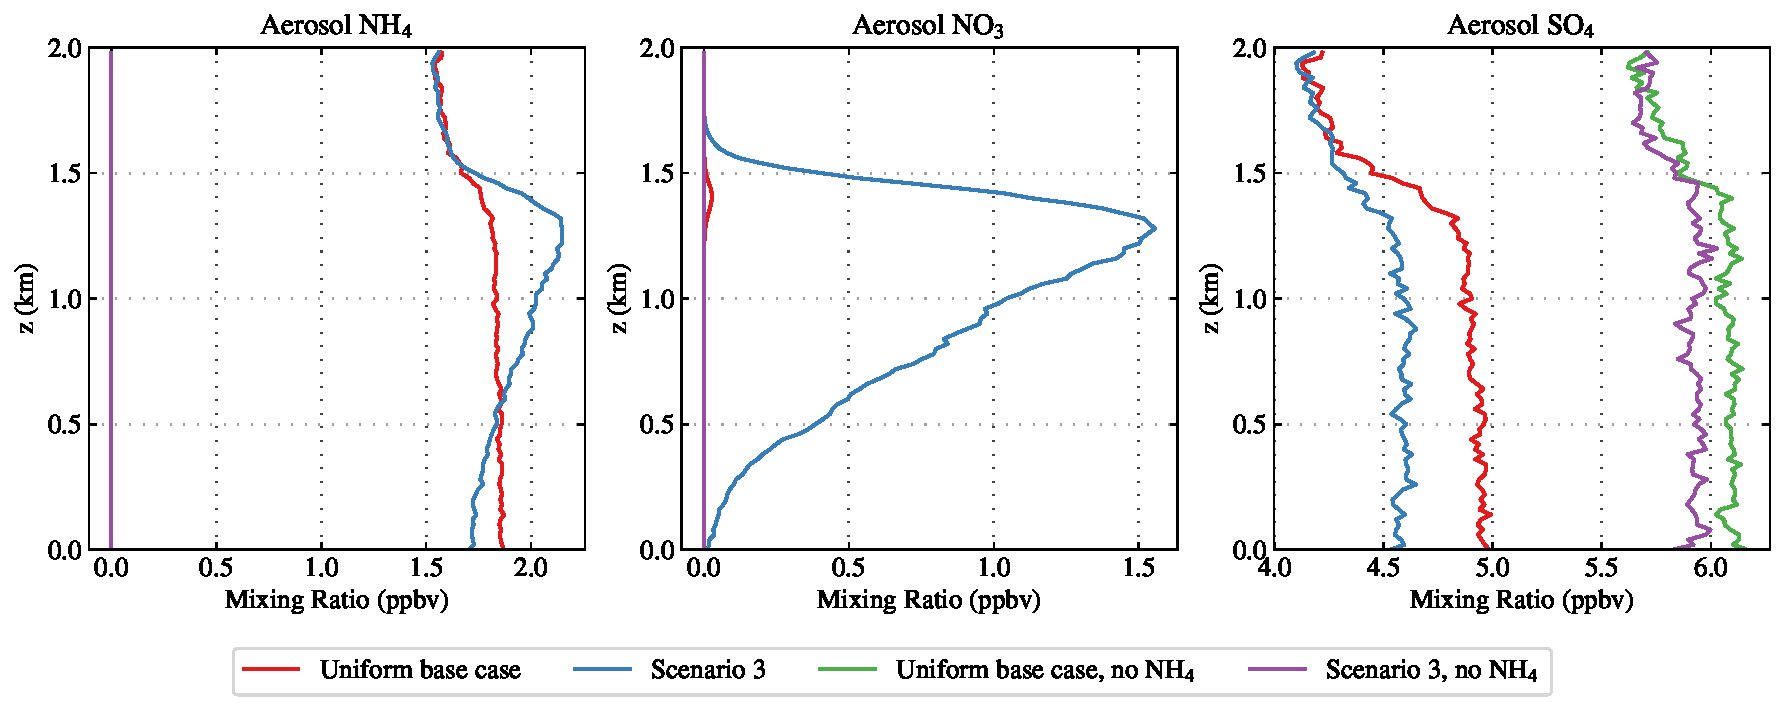
\includegraphics[width=\textwidth]{figures/chapter5/aerosol-SNA-vertical-profiles-no-nh4-cases-time36.pdf}
    \caption{Vertical profiles ($t=6$ h) for ammonium, nitrate, and sulfate comparing uniform base case and scenario~3 both with and without ammonium.}
    \label{fig:vert-profiles-no-nh4}
\end{figure}

Figure \ref{fig:vert-profiles-no-nh4} shows vertical profiles at $t=6$ h for aerosol ammonium, nitrate, and sulfate concentrations in ppbv for four simulation runs: the uniform base case and scenario~3 as shown in previous sections and the same scenarios but without any ammonium present. Simulations with ammonium show that the uniform base case has slightly more ammonium in the lowest 500 m of the planetary boundary layer, while scenario~3 has higher concentrations in excess of 2 ppbv in the middle to upper planetary boundary layer. As a consistency check, the same scenarios without ammonium (uniform base case in green, scenario~3 in purple) indicate zero ammonium throughout the entire domain. We find that simulations without ammonium contain no nitrate, which is consistent with previous discussion of the availability of free ammonia in order to allow nitrate to enter the aerosol phase. Without ammonium present, sulfate concentrations increase for both the uniform base case (4.9 ppbv to 6.1 ppbv) and scenario~3 (4.6 ppbv to 5.9 ppbv). The increase in sulfate between the ammonia-present scenarios and the ammonia-free scenarios can be attributed to changes in the aerosol initial condition; whereas the aerosol is a mixture of 50\% ammonium sulfate and 50\% OC in the ammonia-present scenarios, the ammonia-free scenarios use an initial mixture of 50\% sulfate and 50\% OC, thus the mass concentration of sulfate is greater in ammonia-free scenarios. The decrease of approximately 0.2 ppbv in sulfate concentrations between the uniform base case (green line) without ammonia and the corresponding scenario 3 (purple line) exhibit a similar pattern to the decrease in sulfate across ammonia-present scenarios. Under high emissions spatial heterogeneity scenarios, the elevated concentrations of reactive species in the emitted plume result in significantly greater removal of OH when compared to low heterogeneity scenarios. This effectively slows the rate at which SO$_2$ is oxidized to form H$_2$SO$_4$ which rapidly partitions into the aerosol phase as sulfate. 

\begin{figure}[!t]
  \centering
    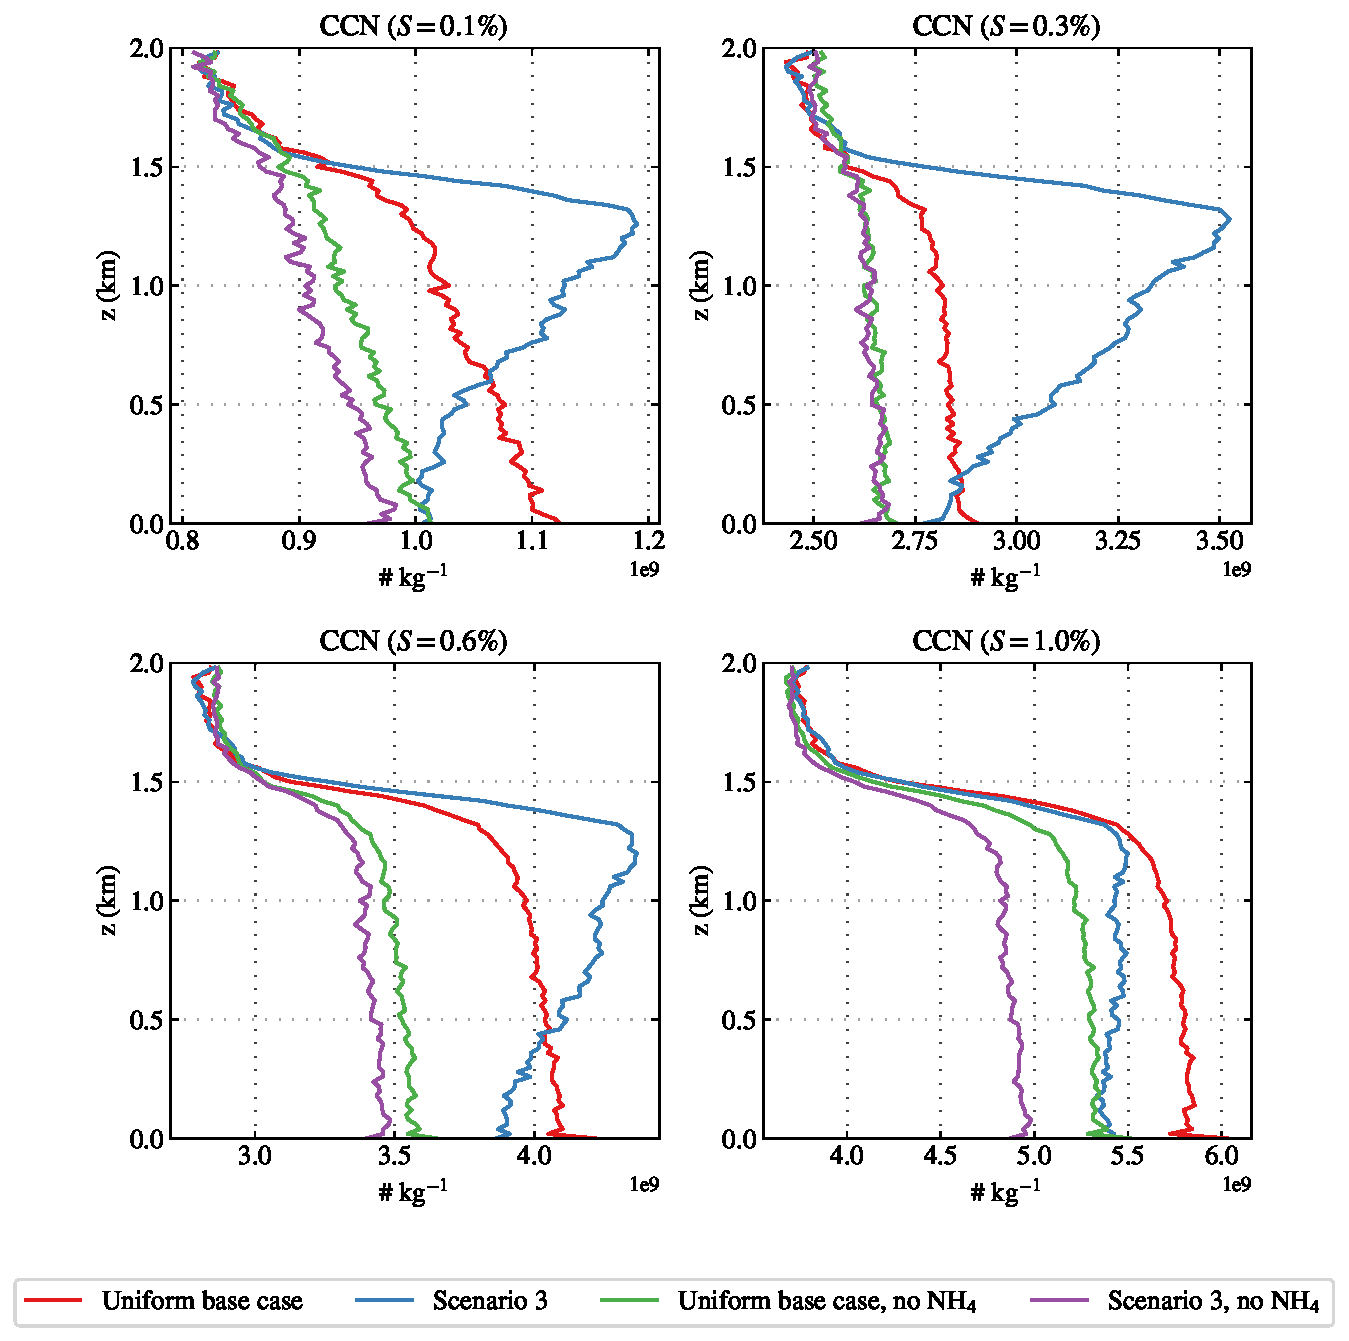
\includegraphics[width=\textwidth]{figures/chapter5/aerosol-ccn-vertical-profiles-no-nh4-cases-time36.pdf}
    \caption{Vertical profiles ($t = 6$ h) for CCN concentrations at supersaturations S = 0.1, 0.3, 0.6, 1.0\% for the uniform base case and scenario~3 with and without ammonium.}
    \label{fig:vert-profiles-ccn-no-nh4}
\end{figure}

Figure \ref{fig:vert-profiles-ccn-no-nh4} shows vertical profiles of CCN number concentrations in number of particles per kilogram of dry air (\# \si{kg^{-1}}) at $t=6$ h for each supersaturation level (S = 0.1, 0.3, 0.6, 1.0\%) for both the uniform base case and emissions scenario~3 with and without ammonium. We find that in the absence of ammonium, concentrations of CCN at each supersaturation level agree closely across the uniform base case and scenario~3. For $S=0.1\%$, we find that CCN concentrations in scenario~3 (no ammonium) are a constant factor of $0.02\cdot10^{9}$~\#~\si{kg^{-1}} less than in the uniform base case (no ammonium). At $S=0.3\%$, CCN concentrations across both scenarios are virtually identical to within random variability. For $S=0.6\%$, the no-ammonium scenario~3 has a relatively constant factor of $0.1\cdot10^{9}$~\#~\si{kg^{-1}} less CCN than the no-ammonium uniform base case. We find a similar relationship for $S=1.0\%$ with a constant factor of $0.5\cdot10^{9}$~\#~\si{kg^{-1}} fewer CCN in the ammonium-free scenario~3 case. 

Simulations without ammonium suggest that the coupling between emissions $SH$ and CCN activity is highly dependent on the composition of both the gas phase and aerosol state. Without the presence of ammonium, no nitrate enters the aerosol particles, reducing their hygroscopicity and resulting CCN activity. Under such conditions, the effect of particle removal by coagulation on CCN activity outweighs changes due to gas-particle partitioning effects on aerosol hygroscopicity. 

%\hl{I think it would be helpful here to include profiles of total number concentration > 50~nm (could also do this elsewhere). My thinking is that coagulation is probably reducing the total number of particles in the high heterogeneity case and this leads to the lower CCN conc. I think this is somewhat counteracted by the increased hygroscopicity of particles in the set of scenarios with ammonium/nitrate present in the aerosol.}

\section{Implications}

We have shown that there exist numerous couplings between emissions spatial heterogeneity and non-linear aerosol processes including coagulation and gas-particle partitioning. These processes alter the aerosol population; coagulation removes particles from the ultrafine Aitken mode due to collision with larger accumulation mode particles while gas-particle partitioning has a significant impact on aerosol composition and associated properties such as particle hygroscopicity. Here, we discuss implications regarding the impact of emissions spatial heterogeneity on the aerosol state and their application to relevant avenues of study. 

In this study, all of the aerosol emission modes utilized in this thesis including cooking, diesel and gas vehicle emissions contain geometric mean diameters smaller than 0.1~$\mu m$. Such particles are referred to as ultrafine aerosol particles. Ultrafine particles are known to have deleterious effects on human health, resulting in respiratory inflammation and increased rates of asthma. Furthermore, ultrafines are capable diffusing across cellular membranes and can be transported throughout the body through the cardiovascular system, resulting in cardiovascular disease and excess mortality due to cardiovascular ailments \parencite{schraufnagel_health_2020}. As shown through idealized coagulation simulations and in discussion of number distributions for full multiphase simulations, coagulation is the primary mechanism for the removal of ultrafine particles. Furthermore, we find that the non-linear nature of coagulation results in enhanced particle removal for emissions scenarios with high spatial heterogeneity. As such, the coupling between emissions spatial heterogeneity and coagulation is of particular importance to human health and efforts to monitor air quality via chemical transport models. Models such as the United States Environmental Protection Agency's (U.S. EPA) Community Multiscale Air Quality Model (CMAQ) are used to monitor regional compliance with regulatory standards for pollutants such as particular matter as set forth in the Clean Air Act \parencite{development_cmaq_2022}. Such models are often run at the regional scale down to resolutions on the order of a few kilometers and as a result do not capture the full spatial heterogeneity of emissions. Furthermore, regional scale chemical transport models such as CMAQ do not include sub-grid scale parameterizations for coagulation \parencite{murphy_communication_2024}. Our findings suggest that regions of highly heterogeneous emissions may result in fewer ultrafine particles in the vicinity of the emitted plume due to the enhanced rate of coagulation. As a result, models such as CMAQ likely misrepresent the size and number concentration of ultrafine particles near emissions sources. This underscores the need to extend the use of sub-grid scale parameterizations such as methods developed by \textcite{pierce_parameterization_2009} and \textcite{sakamoto_evolution_2016} to air quality modeling applications. Our findings are of particular relevance to modeling wildfire plumes which emit ultrafine primary organic aerosol over regions which are often far smaller than the grid resolution of regional and global scale models. 

We find that under low supersaturations ($S=0.3\mbox{--}0.6\%$), CCN activity increases by up to 25\% in the upper boundary layer for emissions scenarios with high spatial heterogeneity. These findings have important implications for global climate models (GCMs) in which emissions are assumed uniform and diffuse over large grid cell regions typically on the order of 100~km. These results may suggest that near regions with highly heterogeneous emissions, current GCMs may underestimate the concentration of CCN. We wish to acknowledge that given the simplifying assumptions of our model setup (see Chapter 3 for detailed discussion), these findings should not be used to draw strict conclusions for climate models, but rather point towards underlying process level changes due to high emissions spatial heterogeneity, such as increased partitioning of ammonium and nitrate into the aerosol and the corresponding increase to aerosol hygroscopicity. In Chapter 1, we discussed a study by \textcite{weigum_effect_2016} which evaluated the sub-grid variability of CCN concentrations and AOD. The authors similarly found that higher resolution simulations led to greater nitrate concentrations when compared to the base resolution representative of GCM grid scales. In addition to the effects of nitrate on increasing aerosol hygroscopicity and subsequent CCN activity (thereby modifying indirect radiative effects), \textcite{weigum_effect_2016} noted that recent GCMs have begun to include nitrate aerosol in the calculation of direct radiative effects. Thus, our findings bolster the importance of improved representation of nitrate aerosol in GCMs and continued efforts to improve representation of sub-grid scale processes such as gas-particle partitioning which alters aerosol composition and climate relevant properties.


%Non-linear coupling between emissions $SH$ and CCN activity, mediated by the presence of nitrate and contingent on the availability of free ammonia to allow partitioning of nitrate into the aerosol phase.

%Idealized coagulation simulations indicate that higher emissions spatial heterogeneity leads to a higher rate of coagulation due to increased number concentration. Correspondingly, number distributions for full mulitphase chemistry simulations indicate a reduction in smaller emission-mode particles and a shift to larger particles likely in part due to enhanced coagulation.

%Sulfate concentrations are lower for high emissions heterogeneity scenarios. This results from the partitioning of less H$_2$SO$_4$ into the aerosol phase. Because H$_2$SO$_4$ possesses a very low volatility vapor pressure, nearly all available H$_2$SO$_4$ will enter the aerosol to form sulfate. This indicates that the availability of sulfate is controlled by the gas phase oxidation of SO$_2$ to form H$_2$SO$_4$ via OH, and that less OH reacts with SO$_2$ under high emissions heterogeneity scenarios. 

%There are numerous contributing factors which alter the availability of OH, first of which is the emissions heterogeneity of the plume. In high heterogeneity scenarios where concentrations in the emissions plume are very high, OH near the vicinity of the plume will rapidly react with the plume constituents including SO$_2$, NO$_x$, and VOCs. This quickly strips the availability of OH in the core of the plume. Reactions including photolytic processes outside the plume that produce OH are not able to replenish the concentration of OH near the plume due to an inability to mix and entrain OH into the plume fast enough. As a result, OH is chemically segregated from its reactants in the plume including SO$_2$. 

%In addition to impacts of emissions plume spatial heterogeneity and chemical segregation, the availability of OH in high emissions heterogeneity scenarios may also be reduced due to lower concentrations of ozone as found in chapter 4. The photolysis of ozone into singlet oxygen and subsequent reaction with H$_2$O is an important formation mechanism for OH. In addition to the mechanism responsible for the reduction in the abundance of ozone discussed in chapter 4, it is likely that aerosols alter the rate of photolysis reactions by increased scattering and absorption of radiation. As many formation mechanisms for OH require photolysis, high concentrations of aerosol particles likely reduces the effective rate at which photolytic reactions occur, especially near the emissions plume. 

%We find that both ammonium and nitrate concentrations increase with emissions spatial heterogeneity, particularly in the upper boundary layer.  Note that most ammonium and nitrate are present in the aerosol phase as ammonium nitrate, which forms via the gas-solid equilibrium reaction between nitric acid and ammonia in the gas phase to form solid ammonium nitrate. Note that nitric acid forms by reacting OH with NO$_2$. The higher concentrations of NO$_2$ observed for high emissions spatial heterogeneity scenarios in chapter 4 indicates an increase in nitric acid (if there is enough OH). The nitric acid-ammonium equilibrium reaction is highly sensitive to temperature with more ammonium nitrate formation at lower temperatures. This helps explain why ammonium and nitrate levels are the highest in the upper boundary layer. Furthermore, the decrease in sulfate under high emissions heterogeneity indicates there is more free ammonia in the aerosol which may neutralize nitric acid by forming ammonium nitrate. 

%We find a complex non-linear coupling between emissions $SH$ and CCN activity which is mediated by aerosol processes including coagulation and gas-particle partitioning. These processes have competing effects on the number concentration of CCN. Coagulation alters the size distribution by effectively removing small particles that activate at high supersaturations. Simultaneously, gas-particle partitioning alters the hygroscopicity of the aerosol by allowing the formation of nitrate, contingent on the availability of free ammonia as discussed previously. This contributes most to an increase in CCN activity at lower supersaturations (S=0.1--0.3\%), as these particles tend to be larger (less likely to be removed by coagulation) and are more hygroscopic. 

%Simulations without ammonium suggest that the coupling between emissions $SH$ and CCN activity is highly dependent on the composition of both the gas phase and aerosol state. Without the presence of ammonium, no nitrate enters the aerosol particles, reducing their hygroscopicity and resulting CCN activity. Under such conditions, the effect of particle removal by coagulation on CCN activity outweighs changes due to gas-particle partitioning effects on aerosol hygroscopicity. 






% !TEX root = ./main.tex
\chapter{Conclusions}

\section{Study limitations and future work}
\hl{Some rough draft ideas}
\begin{itemize}
\item In this study, all emissions are released at the ground level. This is a simplification as some emission sources such as stack emissions from industrial sources are emitted at some height above the surface. Because the atmospheric stability often differs between the surface level and the planetary boundary layer, one may expect the shape and structure of the plume to differ if emissions are released directly into the boundary layer. For example, consider a nocturnal boundary layer/surface layer. If the emissions are released directly into the surface layer capped by a strong nocturnal inversion then emissions in the surface layer will be trapped and concentrations will be very high. If emissions are released from a plume above the surface layer, the absence of vertical mixing will lead to large concentration gradients between the region near the emissions plume and the surrounding ambient conditions. 

\item This thesis investigates the impact of emissions spatial heterogeneity on ccn activity, however one may wish to extend this analysis to include aerosol optical properties which govern their radiative effects.

\item Through the use of particle-resolved modeling in a large-eddy simulation framework, this thesis establishes a benchmark for high resolution representation of aerosol processes in the boundary layer. A natural extension would be to conduct simulations with similar setups but instead use coarser-resolved treatments for the aerosols (e.g., modal or sectional representations) as well as the transport and turbulence treatment (e.g., use of Reynolds Averaged Navier Stokes modeling). This would allow intercomparison with the high-resolution results presented in this thesis and quantify structural uncertainties in desired quantities (such as CCN activity or aerosol optical properties) introduced by the use of coarser-resolved modeling treatments.
 
\item Here we chose spatial and temporal discretization apriori, mainly on the basis of what is feasible given our computational resources. A limitation of this approach is that we are uncertain whether we are adequately resolving all spatial and temporal scales at which gas phase and aerosol chemical reactions occur. Future work should quantitatively determine the necessary spatial and temporal scales for resolving relevant atmospheric chemistry reactions via metrics such as the damkohler number.


\end{itemize}

% test cite
%\cite{Childish07}




% per Graduate College preference, place the \appendix and the appendices content before the
% bibliography (here) only if the appendices contain references.

\backmatter

\printbibliography[heading=bibintoc,title={References}]

%\bibliographystyle{IEEEtran}
%\printbibliography

% the below lines are only needed if bibliography precedes appendices
% uses https://tex.stackexchange.com/a/440212 to continue page numbering
\clearpage
\setcounter{counterforappendices}{\value{page}}
\mainmatter
\setcounter{page}{\value{counterforappendices}}

\appendix

%\chapter{An appendix}

%\lipsum[1-5]

% \input{Appendix.tex}

\end{document}
